\documentclass[a4paper]{article}

\usepackage{amsmath}
\usepackage{amsfonts}
\usepackage{graphicx}
\usepackage{hyperref}
\usepackage[usenames,dvipsnames]{color}

\setlength{\parindent}{0pt}
\setlength{\parskip}{0.75ex plus 0.5ex minus 0.3ex}
\setcounter{secnumdepth}{0} % Do not number sections
\setcounter{tocdepth}{2}

\newcommand{\sympy}{\textbf{\texttt{\textcolor{OliveGreen}{SymPy}} }}
\newcommand{\cmd}[1]{\textbf{\texttt{\textcolor{blue}{#1}}}}


\begin{document}
% ******************************************************************************
\title{Linear Algebra Step by Step in \sympy}

\author{Dario Beraldi}
\maketitle
\tableofcontents

\begin{abstract}
\noindent Excerpts from \textit{Linear Algebra Step by Step} by K. Singh 
with \sympy implementation.
\end{abstract}

% ==============================================================================

Start session with interactive \texttt{python} as:

\begin{verbatim}
ipython
from sympy import *
from matplotlib import pylab as plt

init_printing()
\end{verbatim}

Starting \texttt{isympy} seems to interfere with \texttt{matplotlib} later.

\section{1. Linear Equations and Matrices}
% ========================================

\subsection{Solving linear systems}
% ---------------------------------

\subsubsection{Exercises 1.1 2f} 
% ...............................

\begin{equation}\label{eq:ex2f}
    \begin{matrix}
    e x - e y = 2 \\
    e x + e y = 0
    \end{matrix}
\end{equation}

\begin{verbatim}
x, y= symbols('x y', real= true)
eq1= Eq(E*x - E*y, 2)
eq2= Eq(E*x + E*y, 0)
sols= solve([eq1, eq2])
\end{verbatim}

Solved for:

\begin{equation}\label{eq:ex2fsol}
\begin{Bmatrix}x : e^{-1}, & y : - \frac{1}{e}\end{Bmatrix}
\end{equation}

Check solutions by substituting them in the original equations \ref{eq:ex2f}

\begin{verbatim}
eq1.subs(sols)
True
eq2.subs(sols)
True
\end{verbatim}

Solve the system \ref{eq:ex2f} using matrix notation

\begin{verbatim}
coeffs= Matrix([[E, -E], [E, E]])
const= Matrix([2, 0])
[coeffs, const]
\end{verbatim}

\begin{equation}\label{eq:na}
\begin{bmatrix}\left[\begin{matrix}e & - e\\e & e\end{matrix}\right], & \left[\begin{matrix}2\\0\end{matrix}\right]\end{bmatrix}
\end{equation}

If everything is correct, solutions are consistent with \ref{eq:ex2fsol}:

\begin{verbatim}
coeffs.solve(const)
\end{verbatim}

\begin{equation}
\left[\begin{matrix}e^{-1}\\- \frac{1}{e}\end{matrix}\right]
\end{equation}

\subsubsection{Exercises 1.1 4a}
Plot the graphs of these linear equations
% .....................................................

\begin{equation}\label{eq:na}
\begin{matrix}2 x + y = 3\\x - y = 7\end{matrix}
\end{equation}

\begin{verbatim}
eq1= Eq(2*x + y, 3)
eq2= Eq(x - y, 7)
\end{verbatim}

Plot

\begin{verbatim}
pp1= plot_implicit(eq1)
pp2= plot_implicit(eq2)
pp1.extend(pp2)
pp1.save('figs/ex4a.pdf')
\end{verbatim}

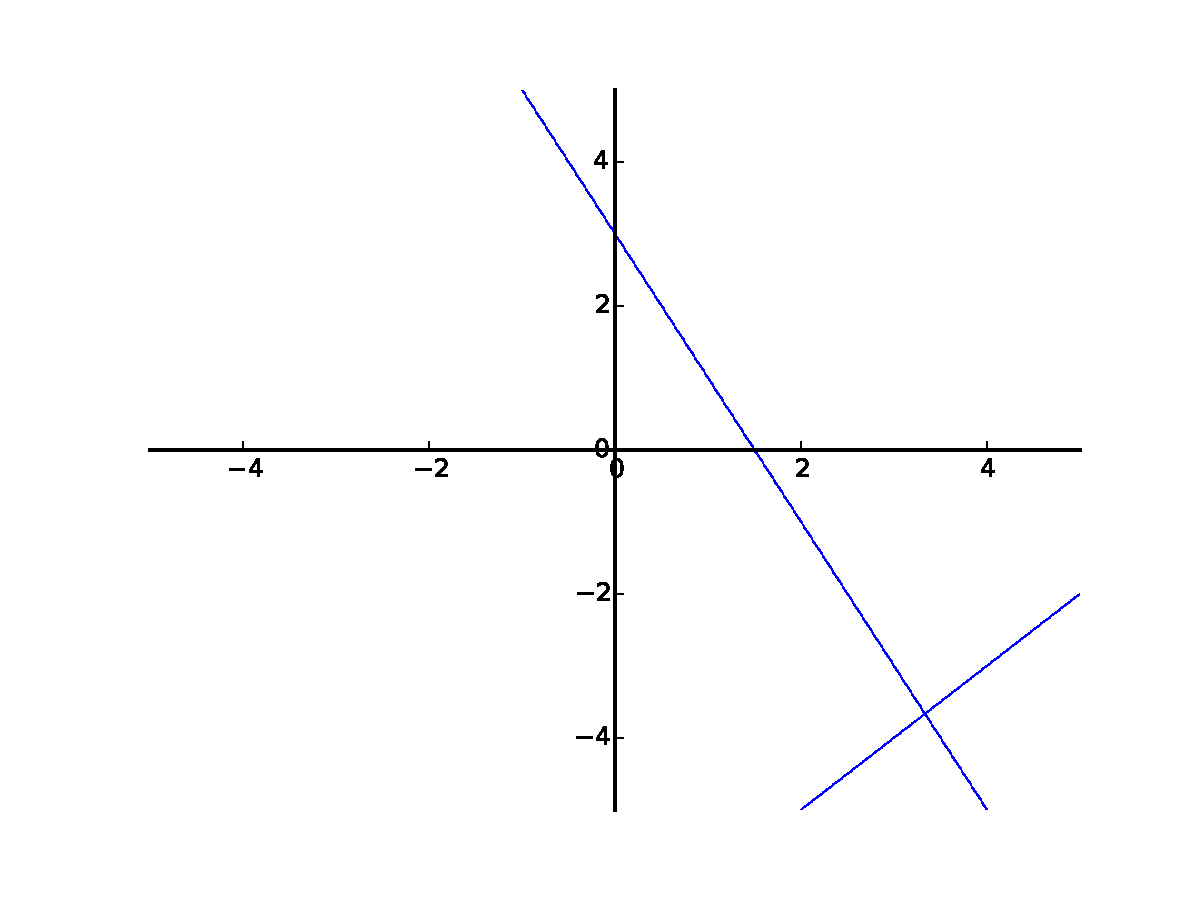
\includegraphics[width=\linewidth]{figs/ex4a.pdf}

\textbf{Exercises 1.1 5b}
% ............

\begin{verbatim}
eq1= Eq(12*x + 4*y, 16)
eq2= Eq(8*x + 4*y, 16)

pp1= plot_implicit(eq1)
pp2= plot_implicit(eq2)
pp1.extend(pp2)
pp1.save('figs/ex5b.pdf')
\end{verbatim}

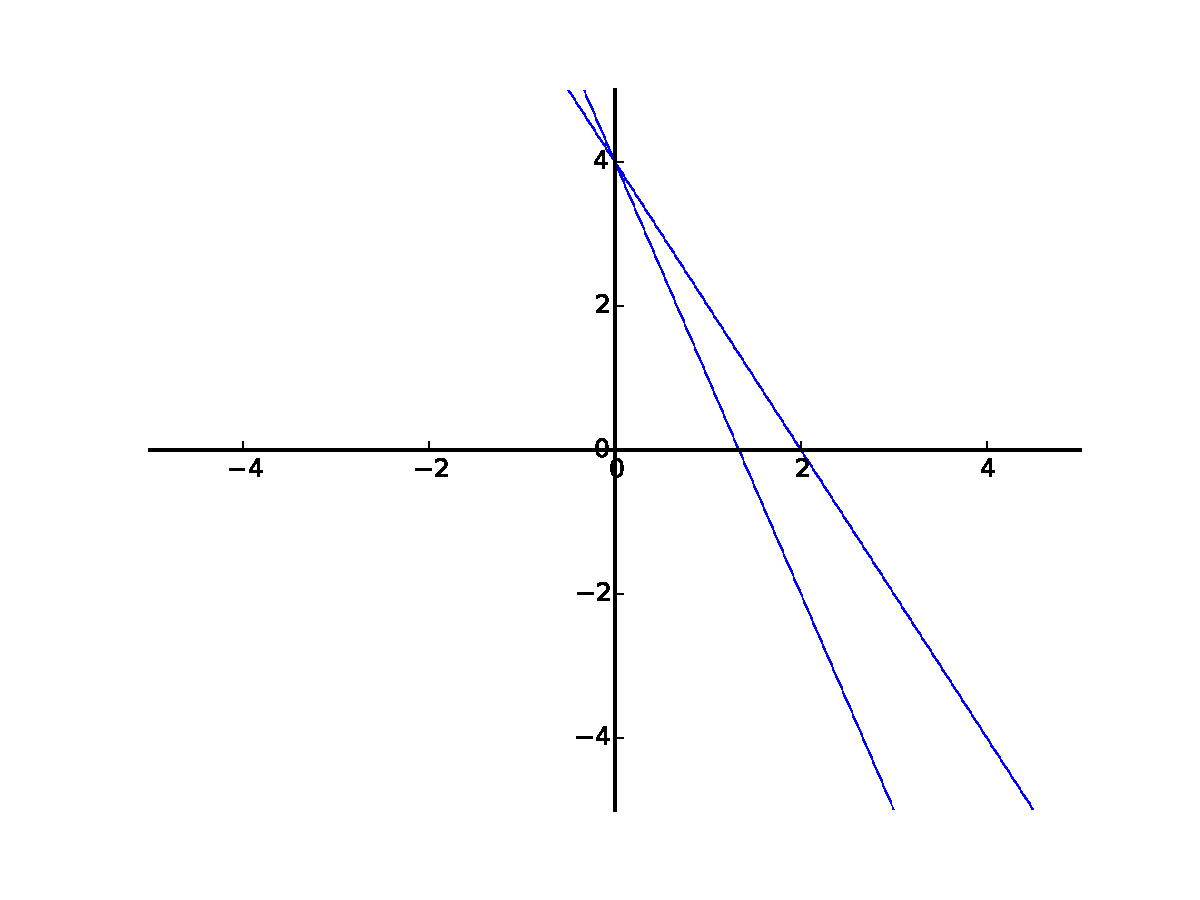
\includegraphics[width=\linewidth]{figs/ex5b.pdf}

\subsection{Solve by row echelon form}
% ------------------------------------

Given a linear system of equations, the solutions can be found by Gaussian
elimination:

\begin{itemize}
\item Extract the coefficients and constants from the equations and put them in
an augmented matrix.
\item Transform the augmented matrix in reduced row echelon form (rref). This is
the result of the Gaussian elimination process.
\item The last columns of the rref matrix lists the solutions of the linear system.
\end{itemize}

Reminder: rref means that every leading coefficient is 1 and is the only nonzero
entry in its column \footnote{http://en.wikipedia.org/wiki/Row\_echelon\_form}. 

\subsubsection{Exercises 1.2 2a}

\begin{equation}\label{eq:na}
\begin{matrix}x + 2 y + 3 z = 12\\2 x - y + 5 z = 3\\3 x + 3 y + 6 z = 21\end{matrix}
\end{equation}

\begin{verbatim}
eq1= Eq(x + 2*y + 3*z, 12)
eq2= Eq(2*x - y + 5*z, 3)
eq3= Eq(3*x + 3*y + 6*z, 21)
\end{verbatim}

Represent the linear systen as \textit{augmented} matrix, where the last column
holds the constants:

\begin{equation}\label{eq:na}
M= \left[\begin{matrix}1 & 2 & 3 & \textit{12}\\
                       2 & -1 & 5 & \textit{3}\\
                       3 & 3 & 6 & \textit{21}\end{matrix}\right]
\end{equation}

In \sympy use the \href{http://docs.sympy.org/latest/modules/polys/reference.html#sympy.polys.polytools.Poly}{\texttt{Poly}}
class to conveniently extract the coefficients at the left hand side of
the equations:

\begin{verbatim}
M= Matrix([
    Poly(eq1.lhs).coeffs(),
    Poly(eq2.lhs).coeffs(),
    Poly(eq3.lhs).coeffs()
])
const= Matrix([eq1.rhs, eq2.rhs, eq3.rhs])
M= const.col_insert(0, M)
\end{verbatim}

In reduced row echelon form, with indexes of the pivot variables on the right:

\begin{equation}\label{eq:na}
RREF= \begin{pmatrix}\left[\begin{matrix}1 & 0 & 0 & 1\\0 & 1 & 0 & 4\\0 & 0 & 1 & 1\end{matrix}\right], & \begin{bmatrix}0, & 1, & 2\end{bmatrix}\end{pmatrix}
\end{equation}

Solutions can be read from last column of the RREF $\left[\begin{matrix}x:1\\y:4\\z:1\end{matrix}\right]$. Verify the solutions solve
the initial system of equations:

\begin{verbatim}
rref= M.rref()
sols= rref[0].col(-1)

eq1.subs({x:sols[0], y:sols[1], z:sols[2]}) # True
eq2.subs({x:sols[0], y:sols[1], z:sols[2]}) # True
eq3.subs({x:sols[0], y:sols[1], z:sols[2]}) # True

# Or the same returning dict {x: 1, y: 4, z: 1}
solve([eq1, eq2, eq3]) 
\end{verbatim}

\subsubsection{Exercises 1.2 3d}
% ..............................

Linear system:

\begin{equation}\label{eq:na}
\begin{matrix}
    - 2 x + 3 y - 2 z = 8 \\
    - x + 2 y - 10 z = 0 \\
    5 x - 7 y + 4 z = -20
\end{matrix}
\end{equation}

Augmented matrix:

\begin{equation}\label{eq:na}
\left[\begin{matrix}-2 & 3 & -2 & 8\\-1 & 2 & -10 & 0\\5 & -7 & 4 & -20\end{matrix}\right]
\end{equation}

Reduced row echelon form with solutions in the last column:

\begin{equation}\label{eq:na}
\begin{pmatrix}\left[\begin{matrix}1 & 0 & 0 & -3 \\
                                   0 & 1 & 0 & 1 \\
                                   0 & 0 & 1 &
\frac{1}{2}\end{matrix}\right], & \begin{bmatrix}0, & 1, & 2\end{bmatrix}\end{pmatrix}
\end{equation}

In \sympy:

\begin{verbatim}
eq1= Eq(-2*x + 3*y -2*z, 8)
eq2= Eq(-x + 2*y - 10*z, 0)
eq3= Eq(5*x - 7*y + 4*z, -20)

M= Matrix([
    Poly(eq1.lhs).coeffs(),
    Poly(eq2.lhs).coeffs(),
    Poly(eq3.lhs).coeffs()
])
const= Matrix([eq1.rhs, eq2.rhs, eq3.rhs])
M= const.col_insert(0, M)
rref= M.rref()
sols= rref[0].col(-1)

# Checked: {x: -3, y: 1, z: 1/2}
solve([eq1, eq2, eq3])
\end{verbatim}

\subsection{Vector arithmetic}
% ----------------------------

\subsubsection{Exercise 1.3.1}

Given two vectors:

\begin{verbatim}
va= Matrix([2, 0])
vb= Matrix([2, 1])
\end{verbatim}

plot the results of the operations 

\subsubsection{(a-e)}

\begin{verbatim}
vA= va + vb          # [4 1]
vB= va - vb          # [0 -1]
vC= 3 * va           # [6 0]
vD= -1/2 * vb        # [-1 -0.5]
vE= 3*va - 1/2 * vb  # [5 -0.5]
\end{verbatim}

And plot vectors

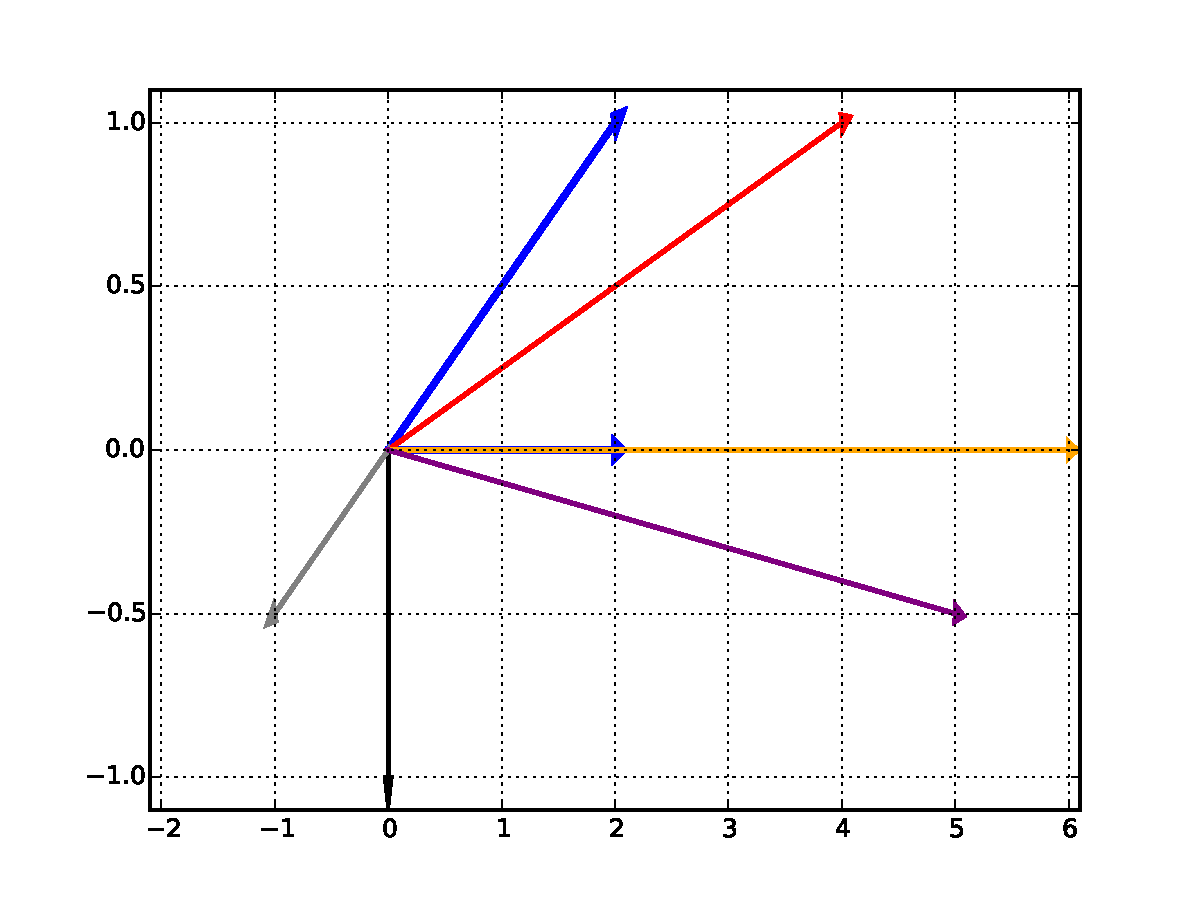
\includegraphics[width=\linewidth]{figs/ex1_3.pdf}

\begin{verbatim}
plt.arrow(0, 0, float(va[0]), float(va[1]), lw= 3, color= 'b', head_width=0.05)
plt.arrow(0, 0, float(vb[0]), float(vb[1]), lw= 3, color= 'b', head_width=0.05)
plt.arrow(0, 0, float(vA[0]), float(vA[1]), lw= 2, color= 'r', head_width=0.05)
plt.arrow(0, 0, float(vB[0]), float(vB[1]), lw= 2, color= 'black', head_width=0.05)
plt.arrow(0, 0, float(vC[0]), float(vC[1]), lw= 2, color= 'orange', head_width=0.05)
plt.arrow(0, 0, float(vD[0]), float(vD[1]), lw= 2, color= 'grey', head_width=0.05)
plt.arrow(0, 0, float(vE[0]), float(vE[1]), lw= 2, color= 'purple', head_width=0.05)
plt.xlim(-2.1, 6.1)
plt.ylim(-1.1, 1.1)
plt.grid()
plt.savefig('figs/ex1_3.pdf')
plt.close()
\end{verbatim}

\subsubsection{Exercise 1.3.8}
% ............................
Show that $x\mathbf{u} + y\mathbf{v} = \mathbf{w}$ where
$\mathbf{u}= (1\ 0)^{T}$, $\mathbf{v}= (0\ 1)^{T}$, and $\mathbf{w}= (x\ y)^{T}$.

This is a consequence of $x(1\ 0) = (x\ 0)$ and $y(0\ 1) = (y\ 0)$. So that
$(x\ 0) + (0\ y) = (x\ y)$

\begin{verbatim}
x, y= symbols('x y')
u= Matrix([1, 0])
v= Matrix([0, 1])
w= Matrix([x, y])
Eq(x*u + y*v, w) # True
\end{verbatim}

\subsubsection{Exercise 1.3.12}
% .............................

Find the real numbers x, y and z, if

\begin{equation}\label{eq:na}
\left[\begin{matrix}x - 2 z\\2 x + y\\- y + 6 z\end{matrix}\right] = \left[\begin{matrix}5\\3\\17\end{matrix}\right]
\end{equation}

Which is solved for:

\begin{equation}\label{eq:}
sols= \begin{bmatrix}\begin{Bmatrix}x : 7, & y : -11, & z : 1\end{Bmatrix}\end{bmatrix}
\end{equation}

\begin{verbatim}
eq1= Eq(x * Matrix([1, 2, 0]) + y * Matrix([0, 1, -1]) + z * Matrix([-2, 0, 6]),
    Matrix([5, 3, 17]))
sols= solve(eq1)
\end{verbatim}

\subsubsection{Exercise 1.3.12}
% .............................

Show that vectors \textbf{u} and \textbf{v} in space $\mathbb{R}^n$ can be
$\mathbf{u} \cdot{} \mathbf{v} = \mathbf{0}$ even if neither \textbf{u} or \textbf{v}
are 0 vectors.

Set:

\begin{verbatim}
u= Matrix([-1, 1])
v= Matrix([1, 1])
u.dot(v) == 0 # True
\end{verbatim}

\subsection{Arithmetic of Matrices}
% ---------------------------------

\subsubsection{Exercise 1.4.1}
% .............................

Given matrix \textbf{B}, note that $3\mathbf{B} = \mathbf{B} + \mathbf{B} + \mathbf{B}$

\begin{equation}
\left[\begin{matrix}6 & -1\\5 & 3\end{matrix}\right]
\end{equation}

\begin{verbatim}
B= Matrix([[6, -1], [5, 3]])
3*B == (B + B + B)
\end{verbatim}

\subsubsection{Exercise 1.4.6}
% .............................

Note how matrx multiplication can result in zero matrix:

\begin{equation}
\left[\begin{matrix}5 & -1 & -2\\10 & -2 & -4\\15 & -3 & -6\end{matrix}\right]
\left[\begin{matrix}1 & 1 & 3\\1 & -1 & -1\\2 & 3 & 8\end{matrix}\right]
= \left[\begin{matrix}0 & 0 & 0\\0 & 0 & 0\\0 & 0 & 0\end{matrix}\right]
\end{equation}

\begin{verbatim}
A= Matrix(3, 3, [5, -1, -2, 10, -2, -4, 15, -3, -6])
B= Matrix(3, 3, [1, 1, 3, 1, -1, -1, 2, 3, 8])
Z= A * B
\end{verbatim}

\subsubsection{Exercise 1.4.8}
% ............................

$\mathbf{x}_n = \mathbf{A}^n\mathbf{x}$ Describes a \textbf{discrete dynamical
system}. Apply this formula to

\begin{equation}\label{eq:ex148}
A = \left[\begin{matrix}0.5 & 0.5\\0.5 & 0.5\end{matrix}\right]
\end{equation}

\begin{verbatim}
A= Matrix(2, 2, [1/2, 1/2, 1/2, 1/2])
\end{verbatim}

For the matrix in \ref{eq:ex148} $A^n = A$:

\begin{verbatim}
A**2 == A # True
A**3 == A # True
A**10 == A # True
\end{verbatim}

matrix in \ref{eq:ex148} is a Markov matrix since the colum sums equal 1.

\subsubsection{Exercise 1.4.10}
% .............................

Determine the image of the matrix \textbf{F} after transformation \textbf{AF}:

\begin{equation}
A = \left[\begin{matrix}1 & 0.2\\0 & 1\end{matrix}\right]
\end{equation}

\begin{equation}
F = \left[\begin{matrix}1 & 1 & 2 & 2 & 1.4 & 1.4 & 2 & 2 & 1.4 & 1.4\\1 & 3 & 3 & 2.6 & 2.6 & 2 & 2 & 1.6 & 1.6 & 1\end{matrix}\right]
\end{equation}

\begin{equation}\label{eq:}
AF = \left[\begin{matrix}1.2 & 1.6 & 2.6 & 2.52 & 1.92 & 1.8 & 2.4 & 2.32 & 1.72 & 1.6\\1 & 3 & 3 & 2.6 & 2.6 & 2 & 2 & 1.6 & 1.6 & 1\end{matrix}\right]
\end{equation}

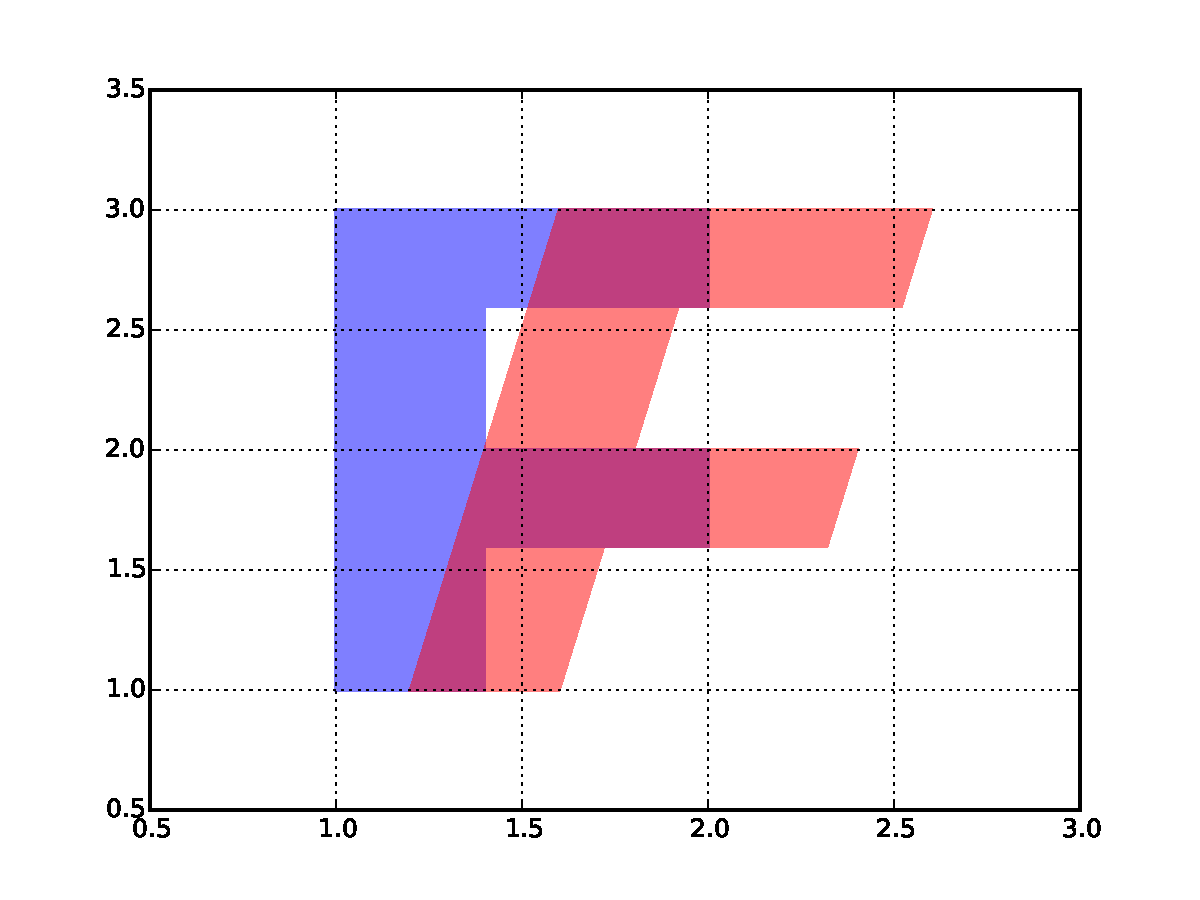
\includegraphics[width=\linewidth]{figs/1_4_10.pdf}

This is showing that the matrix operation $\mathbf{AF} = \mathbf{F_2}$ can be seen as
$\mathbf{f(F)}= \mathbf{F_2}$. That is, the matrix on the left-hand (\textbf{A})
side acts like a function that transforms its argument (\textbf{F}).

\begin{verbatim}
A= Matrix([[1, 0.2], [0, 1]])
F= Matrix([
    [1, 1, 2, 2, 1.4, 1.4, 2, 2, 1.4, 1.4],
    [1, 3, 3, 2.6, 2.6, 2, 2, 1.6, 1.6, 1]])

AF= A*F

verts_F= []
for i in range(F.cols):
    verts_F.append((F[0, i], F[1, i]))
verts_AF= []
for i in range(AF.cols):
    verts_AF.append((AF[0, i], AF[1, i]))

fig = plt.figure()
ax = fig.add_subplot(1, 1, 1)
poly_F = patches.Polygon(verts_F, color= 'b', alpha= 0.5)
poly_AF = patches.Polygon(verts_AF, color= 'r', alpha= 0.5)
ax.set_xlim((0.5, 3))
ax.set_ylim((0.5, 3.5))
ax.add_patch(poly_F)
ax.add_patch(poly_AF)
plt.grid()
plt.savefig('figs/1_4_10.pdf')
\end{verbatim}

\subsubsection{Exercise 1.4.11}
% .............................

\begin{verbatim}
O= Matrix.zeros(2, 1)
X= Matrix([x, y])
\end{verbatim}

\begin{verbatim}
A= Matrix([[1, 2], [3, 5]])
xy= A.solve(O) # x:0, y:0
# Or
xy= A.LUsolve(O) 
# Or
solve(A*X)

A= Matrix([[2, 7], [3, 15]]) # x:0, y:0
xy= A.solve(O)

A= Matrix([[1, 4], [3, 12]]) # Linearly dependent!
xy= A.solve(O)
>>> ValueError: Matrix det == 0; not invertible.
\end{verbatim}

\subsubsection{Exercise 1.4.12}
% .............................

Determine whether vector \textbf{w} is a linear combination of vector \textbf{u}
and \textbf{v}.

Effectively this is asking if the equation $x\mathbf{u} + y\mathbf{v} = \mathbf{w}$
can be resolved.


\begin{itemize}
\item Create an augmented matrix as [u, v, w].
\item Transform the augmented matrix in row echelon form.
\item Get coefficients x and y from last column of RREF. The three vectors are linearly
independent and \textbf{w} $\neq$ \textbf{u} + \textbf{v} (\textbf{w} is not a linear
combination of \textbf{u} and \textbf{v}).

\end{itemize}

\begin{verbatim}
w= Matrix(2, 1, [1, 0])
u= Matrix(2, 1, [5, 8])
v= Matrix(2, 1, [2, 4])
A=  w.col_insert(0, v).col_insert(0, u)
A.rref()
\end{verbatim}

\begin{equation}
REF= \begin{pmatrix}\left[\begin{matrix}1 & 0 & 1\\0 & 1 & -2\end{matrix}\right], & \begin{bmatrix}0, & 1\end{bmatrix}\end{pmatrix}
\end{equation}

\textbf{w} is a linear combination. In fact $1\mathbf{u} -2\mathbf{v}= \mathbf{w}$

\begin{verbatim}
w= Matrix(2, 1, [0, 1])
u= Matrix(2, 1, [5, 8])
v= Matrix(2, 1, [2, 4])
A=  w.col_insert(0, v).col_insert(0, u)
A.rref()
\end{verbatim}

\begin{equation}\label{eq:}
\begin{pmatrix}\left[\begin{matrix}1 & 0 & - \frac{1}{2}\\0 & 1 & \frac{5}{4}\end{matrix}\right], & \begin{bmatrix}0, & 1\end{bmatrix}\end{pmatrix}
\end{equation}

\begin{verbatim}
w= Matrix(3, 1, [1, 2, 3])
u= Matrix(3, 1, [1, 0, 0])
v= Matrix(3, 1, [0, 1, 0])
A=  w.col_insert(0, v).col_insert(0, u)
A.rref()
\end{verbatim}

\begin{equation}
REF= \begin{pmatrix}\left[\begin{matrix}1 & 0 & 0\\0 & 1 & 0\\0 & 0 & 1\end{matrix}\right], & \begin{bmatrix}0, & 1, & 2\end{bmatrix}\end{pmatrix}
\end{equation}

\textbf{w} cannot be a linear combination. In fact
$0\mathbf{u} + 0\mathbf{v} \neq [1\ 2\ 3]^T$

\begin{verbatim}
w= Matrix(3, 1, [1, 2, 3])
u= Matrix(3, 1, [4, 8, 0])
v= Matrix(3, 1, [1, 2, -3/7])
A=  w.col_insert(0, v).col_insert(0, u)
A.rref()
\end{verbatim}

\begin{equation}\label{eq:}
\begin{pmatrix}\left[\begin{matrix}1 & 0 & 2.0\\0 & 1.0 & -7.0\\0 & 0 & 0\end{matrix}\right], & \begin{bmatrix}0, & 1\end{bmatrix}\end{pmatrix}
\end{equation}

\subsection{Matrix Algebra}
% -------------------------

\subsubsection{Exrcises 1.5.2}
% ............................

Given $A = \left[\begin{matrix}5 & -1 & -2\\1 & -3 & 2\end{matrix}\right]$

A) Find \textbf{B} suc that \textbf{A} + \textbf{B} = \textbf{O} with \textbf{O}
a 2 x 3 matrix.

Requires $\mathbf{A} = \mathbf{B} \Rightarrow \mathbf{B} = -\mathbf{A}$

\begin{verbatim}
A= Matrix([[5, -1, -2], [1, -3, 2]])
O= Matrix.zeros(2, 3)
\end{verbatim}


\subsubsection{Exrcises 1.5.7}
% ----------------------------

Determine the scalar $\lambda$ so that $\mathbf{Ax} = \lambda \mathbf{x}$ with
$\mathbf{A} = \left[\begin{matrix}2 & 1 \\ 1 & 2\end{matrix}\right]$ and $\mathbf{x} = \left[\begin{matrix} 1\\1 \end{matrix}\right]$

$\lambda = 3$ since $\mathbf{Ax} = [3\ 3]^T$.

\begin{verbatim}
A= Matrix([[2, 1], [1, 2]])
x= Matrix(2, 1, [1, 1])
l= symbols('lambda')
solve(Eq(A*x, l*x)) # Lambda= 3
\end{verbatim}

\subsubsection{Exrcises 1.5.10}
% ----------------------------

Given \textbf{T} a transition matrix from a Markov chain and \textbf{p} a
probability vector. Note that the probility vector must sum to 1.

What is the probility that the chain is in a given state after $k$ steps?

The answer is given by $\mathbf{p}_k = \mathbf{T}^k\mathbf{p}$.

For:
\begin{equation}
\left[\begin{matrix}0.6 & 0.7\\0.4 & 0.3\end{matrix}\right]
\end{equation}

\begin{equation}
\left[\begin{matrix}0.5\\0.5\end{matrix}\right]
\end{equation}

Determine $\mathbf{p}_k$ for $k$ in 1, 2, 10, 100, 100000:

$p_{k= 1} = \left[\begin{matrix}0.65\\0.35\end{matrix}\right]$

$p_{k= 2} = \left[\begin{matrix}0.635\\0.365\end{matrix}\right]$

$p_{k= 10} = \left[\begin{matrix}0.63636363635\\0.36363636365\end{matrix}\right]$

$p_{k= 100} = \left[\begin{matrix}0.636363636363634\\0.363636363636362\end{matrix}\right]$

$p_{k= 100000} = \left[\begin{matrix}0.636363636361267\\0.36363636363501\end{matrix}\right]$

Note how the probability vector converges in the long period. The probability vector
at the initial state $k = 0$ might represent the proportion of different species
in the environment. Given the probility of change in \textbf{T}, we can ask the question:
What proportion of species we will see after $k$ iterations (\textit{e.g} generations)?

\begin{verbatim}
T= Matrix(2,2, [0.6, 0.7, 0.4, 0.3])
p= Matrix(2, 1, [0.5, 0.5])
ks= [1, 2, 10, 100, 100000]

for k in ks:
    p_k= T**k * p
    print latex(p_k)
\end{verbatim}


\subsection{Type of solutions}
% ========================================

\subsubsection{Exrcises 1.7.8}
% ----------------------------

\begin{equation}\label{eq:}
\textbf{M} = \left[\begin{matrix}1 & 1 & 1 & 0 & 0 & 0 & 6\\0 & 0 & 0 & 1 & 1 & 1 & 15\\1 & 0 & 0 & 1 & 0 & 0 & 5\\0 & 1 & 0 & 0 & 1 & 0 & 7\\0 & 0 & 1 & 0 & 0 & 1 & 9\end{matrix}\right]
\end{equation}

\begin{equation}\label{eq:}
\mathbf{M_{rref}}= \begin{pmatrix}\left[\begin{matrix}1 & 0 & 0 & 0 & -1 & -1 & -10\\0 & 1 & 0 & 0 & 1 & 0 & 7\\0 & 0 & 1 & 0 & 0 & 1 & 9\\0 & 0 & 0 & 1 & 1 & 1 & 15\\0 & 0 & 0 & 0 & 0 & 0 & 0\end{matrix}\right], & \begin{bmatrix}0, & 1, & 2, & 3\end{bmatrix}\end{pmatrix}
\end{equation}

There are six variables with coefficents arranged as in matrix $\mathbf{M}$. In
RREF it appears the first four variables, $x_1$ to $x_4$, have 1 as leading
coefficient, as reported by \sympy in the list of pivot variables indexes on the right
(0, 1, 2, 3). Variables $x_5$ and $x_6$ are \textit{free} with coefficients given
in the respective columns. The solutions are therefore:

\begin{equation}\label{eq:}
\begin{Bmatrix}x_{1} : x_{5} + x_{6} - 10, & x_{2} : - x_{5} + 7, & x_{3} : - x_{6} + 9, & x_{4} : - x_{5} - x_{6} + 15\end{Bmatrix}
\end{equation}

\begin{verbatim}
M= Matrix([
[1, 1, 1, 0, 0, 0, 6],
[0, 0, 0, 1, 1, 1, 15],
[1, 0, 0, 1, 0, 0, 5],
[0, 1, 0, 0, 1, 0, 7],
[0, 0, 1, 0, 0, 1, 9],
])
M_rref= M.rref()
\end{verbatim}

Solve system of equations:

\begin{verbatim}
x1, x2, x3, x4, x5, x6= symbols('x1:7')
r1= Eq(x1 + x2 + x3, 6)
r2= Eq(x4 + x5 + x6, 15)
r3= Eq(x1 + x4, 5)
c1= Eq(x2 + x5, 7)
c2= Eq(x3 + x6, 9)
sols= solve([r1, r2, r3, c1, c2])
\end{verbatim}

\subsubsection{Exrcises 1.7.11}
% ----------------------------

\begin{verbatim}
x, y, z, t= symbols('x y z t', real= True)

eq1= Eq(2*x - 4*y + 4*z + 0.077*t, 3.86)
eq2= Eq(     -2*y + 2*z - 0.056*t, -3.47)
eq3= Eq(2*x - 2*y,                 0)
sols= solve([eq1, eq2, eq3], [x, y, z])
\end{verbatim}

The solutions \texttt{sols}  are in \ref{eq:ex1_7_11}.

Solving via augmented matrix in reduced row echelon form:

\begin{verbatim}
M= Matrix([
    [2, -4, 4, 0.077, 3.86],
    [0, -2, 2, -0.056, -3.47],
    [2, -2, 0, 0, 0]
])
M_rref= M.rref()
\end{verbatim}

\begin{equation}\label{eq:}
\begin{matrix}
2 x - 4 y + 4 z + 0.077 t= 3.86, & \\
- 2 y + 2 z - 0.056 t = -3.47, & \\
2 x - 2 y = 0\end{matrix}
\end{equation}

\begin{equation}\label{eq:}
M= \left[\begin{matrix}2 & -4 & 4 & 0.077 & 3.86\\0 & -2 & 2 & -0.056 & -3.47\\2 & -2 & 0 & 0 & 0\end{matrix}\right]
\end{equation}

\begin{equation}\label{eq:}
M_{rref} = \begin{pmatrix}\left[\begin{matrix}1 & 0 & 0 & 0.0945 & 5.4\\0 & 1 & 0 & 0.0945 & 5.4\\0 & 0 & 1 & 0.0665 & 3.665\end{matrix}\right], & \begin{bmatrix}0, & 1, & 2\end{bmatrix}\end{pmatrix}
\end{equation}

Note that the 4th column holds the coefficients for the free variable $t$ while the
last column has the values for $x, y, z$. Compare to the solutions
from \sympy \texttt{solve}:

\begin{equation}\label{eq:ex1_7_11}
\begin{Bmatrix}x : - 0.0945 t + 5.4, & y : - 0.0945 t + 5.4, & z : - 0.0665 t + 3.665\end{Bmatrix}
\end{equation}

\subsection{The inverse matrix method}
% ====================================

\subsubsection{Exrcises 1.8.3}
% ----------------------------

What effect has the matrix \textbf{E} on the matrix \textbf{A}. With \textbf{A}
a generic 3x3 matrix:

\begin{verbatim}
x1, x2, x3, x4, x5, x6, x7, x8, x9= symbols('x1:10')
k= symbols('k', zero= False)
A= Matrix(3,3, [x1, x2, x3, x4, x5, x6, x7, x8, x9])
\end{verbatim}

\begin{equation}\label{eq:1_8_3A}
\mathbf{A} = \left[\begin{matrix}x_{1} & x_{2} & x_{3}\\x_{4} & x_{5} & x_{6}\\x_{7} & x_{8} & x_{9}\end{matrix}\right]
\end{equation}

\begin{equation}\label{eq:}
\mathbf{E} = \left[\begin{matrix}1 & 0 & 0\\0 & -1 & 0\\0 & 0 & 1\end{matrix}\right]
\end{equation}

\begin{verbatim}
E_a= Matrix([
    [1, 0, 0],
    [0, -1, 0],
    [0, 0, 1]
])
print latex(E_a * A)
\end{verbatim}

\begin{equation}\label{eq:}
\mathbf{E_aA} = \left[\begin{matrix}x_{1} & x_{2} & x_{3}\\- x_{4} & - x_{5} & - x_{6}\\x_{7} & x_{8} & x_{9}\end{matrix}\right]
\end{equation}

\begin{verbatim}
E_b= Matrix([
    [0, 0, 1],
    [0, 1, 0],
    [1, 0, 0]
])
print latex(E_b * A)
\end{verbatim}

\begin{equation}\label{eq:}
\mathbf{E_bA} = \left[\begin{matrix}x_{7} & x_{8} & x_{9}\\x_{4} & x_{5} & x_{6}\\x_{1} & x_{2} & x_{3}\end{matrix}\right]
\end{equation}

\begin{verbatim}
E_c= Matrix([
    [k, 0, 0],
    [0, 1, 0],
    [0, 0, 1]
])
print latex(E_c * A)
\end{verbatim}

\begin{equation}\label{eq:}
\mathbf{E_cA} = \left[\begin{matrix}k x_{1} & k x_{2} & k x_{3}\\x_{4} & x_{5} & x_{6}\\x_{7} & x_{8} & x_{9}\end{matrix}\right]
\end{equation}


\begin{verbatim}
E_d= Matrix([
    [1, 0, 0],
    [0, 1, 0],
    [0, 0, -1/k]
])
print latex(E_d * A)
\end{verbatim}

\begin{equation}\label{eq:}
\mathbf{E_dA} = \left[\begin{matrix}x_{1} & x_{2} & x_{3}\\x_{4} & x_{5} & x_{6}\\- \frac{x_{7}}{k} & - \frac{x_{8}}{k} & - \frac{x_{9}}{k}\end{matrix}\right]
\end{equation}

\subsubsection{Exrcises 1.8.5}
% ----------------------------

Solve the linear systems using inverse matrix method.

\begin{equation}\label{eq:eqs_1_8_5}
\begin{matrix}x + 2 y = 3, & \\ - x + 4 y = 5\end{matrix}
\end{equation}

The coefficients on the LHS of the equations can be thought as a matrix
\textbf{A}. \textbf{A} transforms the vector of unknown coefficients \textbf{x}
to produce the vector of constants \textbf{b} on the RHS:

\begin{equation}\label{eq:1_8_5}
\mathbf{A}\mathbf{x} = \mathbf{b}
\end{equation}

To find the vector \textbf{x} we can rearrange \ref{eq:eqs_1_8_5} as:

\begin{equation}
\mathbf{x} = \mathbf{A}^{-1}\mathbf{b}
\end{equation}

In case of \ref{eq:eqs_1_8_5} we have $\mathbf{A} = \left[\begin{matrix}1 & 2\\-1 & 4\end{matrix}\right]$,
$\mathbf{b} = \left[\begin{matrix}3\\5\end{matrix}\right]$. So
$\mathbf{A^{-1}} = \left[\begin{matrix}\frac{2}{3} & - \frac{1}{3}\\\frac{1}{6} & \frac{1}{6}\end{matrix}\right]$
and $\mathbf{x} = \mathbf{A^{-1}b} = \left[\begin{matrix}\frac{1}{3}\\\frac{4}{3}\end{matrix}\right]$

\begin{verbatim}
x, y= symbols('x y')
eq1= Eq(x + 2*y, 3)
eq2= Eq(-x + 4*y, 5)

A = Matrix(2, 2, [1, 2, -1, 4])
b = Matrix(2, 1, [3, 5])
Ai= A.inv()
x= Ai * b
\end{verbatim}

In case of $\mathbf{Ax = b}$ as:

\begin{equation}\label{eq:}
\left[\begin{matrix}1 & 0 & 2\\2 & 3 & 1\\3 & 6 & 0\end{matrix}\right]
\mathbf{x} = 
\left[\begin{matrix}-1\\1\\9\end{matrix}\right]
\end{equation}

Matrix \textbf{A} is not invertible and the system has no solutions.

\begin{verbatim}
A = Matrix([
[1, 0, 2],
[2, 3, 1],
[3, 6, 0]
])
b= Matrix(3, 1,  [-1 , 1, 9])

Ai= A.inv()
# ValueError: Matrix det == 0; not invertible.
\end{verbatim}

\subsubsection{Exrcises 1.8.7}
% ----------------------------

\textbf{Leontief input-output model}. Represents the production \textbf{p} and
demand \textbf{d} as a matrix. \textbf{p} and \textbf{d} are vectors where each entry
represents a good. The production of goods is represented as a matrix where each row
states how much units of the other goods (input) is required to produce one unit
of that good (output). With this model we can ask how much input is needed to produce
a given amount of output.

$$
\bordermatrix{\text{}& O & E & S \cr
                 O & 0.25 &  0.15  & 0.1 \cr
                 E & 0.4  &  0.15  & 0.2 \cr
                 S & 0.15 &  0.2   & 0.2} = \mathbf{A}
$$

Reading this matrix row by row, it tells how much Oil, Energy and Services it is
needed to produce one unit of O, E, or S. For example 1 unit of O requires 0.25 units
of O, 0.15 of E and 0.1 units of S.

From this matrix we can relate the production vector \textbf{p} to the demand
vector \textbf{d} as:

\begin{equation}\label{eq:1_8_7io}
\mathbf{p} = \mathbf{Ap} + \mathbf{d}
\end{equation}


We want to know \textbf{p} given \textbf{A} and the demand vector \textbf{d}.
\emph{I.e.} we want to solve \ref{eq:1_8_7io} \emph{w.r.t.} \textbf{p} by re-arranging
to the form \textbf{Ax = b}.

$$\mathbf{
p - Ap = d
}$$

then use the identity matrix to obtain the solvable form \textbf{Ax = b}:

$$\mathbf{
p(I - A) = d
}$$

Now solve by inverting \textbf{(I - A)}:

$$\mathbf{
p = (I - A)^{-1} d
}$$

If the demand for O, E, and S is $\mathbf{d} = [100, 100, 100]^T$ we need to
produce
$\left[\begin{matrix}O \\ E \\ S \end{matrix}\right] = \left[\begin{matrix}220 \\ 276 \\ 235 \end{matrix}\right]$

\begin{verbatim}
A = Matrix([
[0.25, 0.15, 0.1],
[0.4, 0.15, 0.2],
[0.15, 0.2, 0.2]
])

d= Matrix(3, 1, [100, 100, 100])
ii= eye(A.rows)
p= (ii - A).inv() * d
\end{verbatim}



\subsubsection{Exrcises 1.8.8}
% ----------------------------

Show that if \textbf{A} is invertible then $A^Tx=b$ has a unique solution.

\begin{verbatim}
x1, x2, x3, x4, x5, x6, x7, x8, x9= symbols('x1:10')
A= Matrix(3,3, [x1, x2, x3, x4, x5, x6, x7, x8, x9])

k1, k2, k3= symbols('k1:4')
b= Matrix(3, 1, [k1, k2, k3])

A_rref= A.transpose().solve(b).rref()
\end{verbatim}

\begin{equation}\label{eq:}
\mathbf{A_{rref}} = \begin{pmatrix}\left[\begin{matrix}1\\0\\0\end{matrix}\right], & \begin{bmatrix}0\end{bmatrix}\end{pmatrix}
\end{equation}

\textit{Does it mean there is a unique solution?}
\section{2. Euclidean Space}
% **************************

\subsection{Properties of vectors}
% ================================

Dot product, norm and distances. The dot product of two vectors \textbf{A} and
\textbf{B} can be thought as the prodcut of their magnitude times the angle between
them:

$$\mathbf{A} \cdot \mathbf{B} = \|\mathbf{A}\| \cdot \|\mathbf{B}\|cos(\theta)$$

Since $cos(\pi/2) = 0$, if the two vectors are orthogonal their dot product is
0. For example $\left[\begin{matrix}2\\0\end{matrix}\right] \cdot \left[\begin{matrix}0\\2\end{matrix}\right] = 0$

\subsubsection{Exercise 2.1.1}
% ----------------------------

Evaluate

\begin{verbatim}
import matplotlib.pyplot as plt

u= Matrix(2, 1, [-1, 3])
v= Matrix(2, 1, [2, 1])

plt.text(float(u[0])+0.2, float(u[1]), 'u', fontsize= 30, color= 'r')
plt.text(float(v[0])-0.2, float(v[1]), 'v', fontsize= 30, color= 'r')
plt.arrow(0, 0, float(u[0]), float(u[1]), lw= 3, color= 'b', head_width=0.05)
plt.arrow(0, 0, float(v[0]), float(v[1]), lw= 3, color= 'b', head_width=0.05)
plt.xlim((-1.1, 3.1))
plt.ylim((-1.1, 3.1))
plt.grid()
plt.savefig('figs/ex2_1_1.pdf')
plt.close()
\end{verbatim}

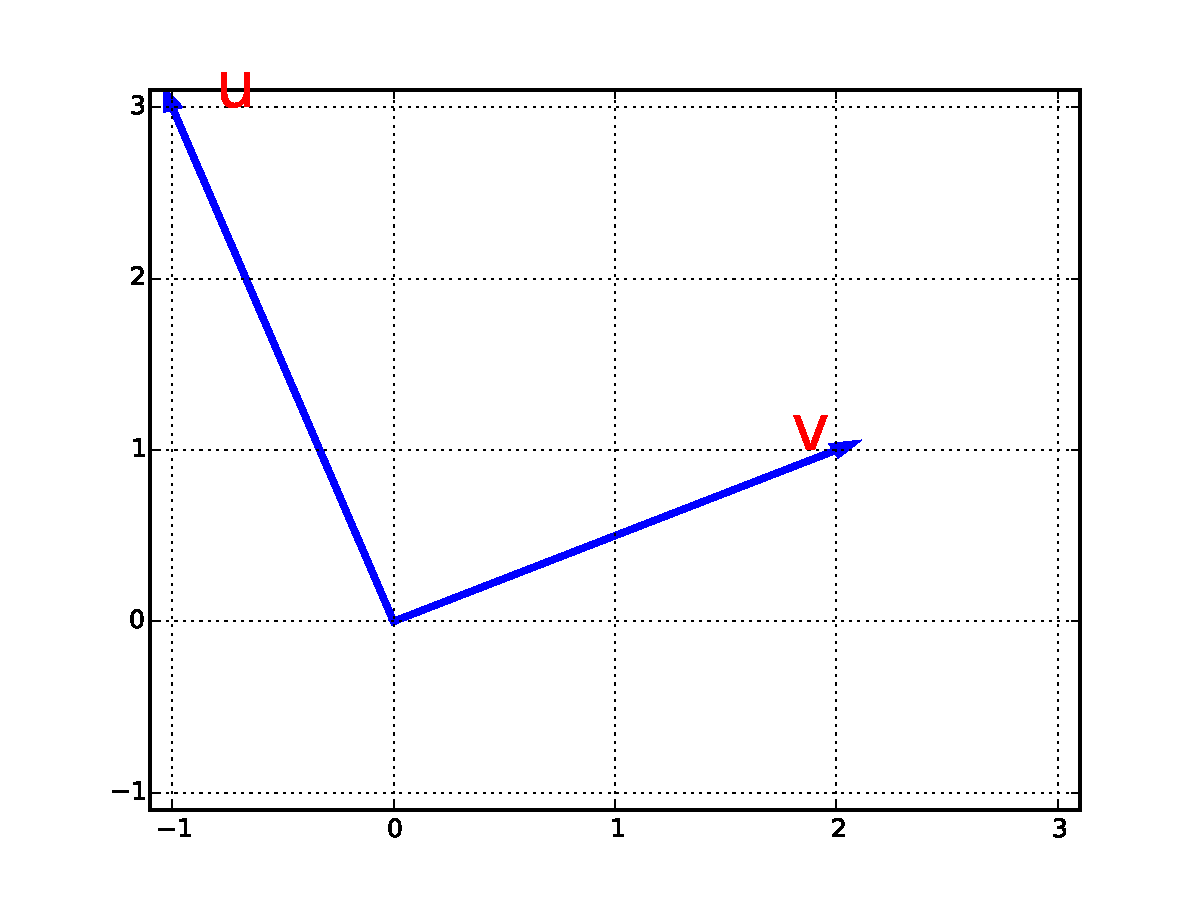
\includegraphics[width=\linewidth]{figs/ex2_1_1.pdf}

\begin{verbatim}
u.dot(v) # 1
v.dot(u) # 1
u.dot(u) # 10
v.dot(v) # 5

u.norm()            # sqrt(10)
u.norm()**2         # 10
v.norm()            # sqrt(5)
v.norm()**2         # 5
(u + v).norm()**2   # 17
(u - v).norm()      # sqrt(13)
\end{verbatim}

\subsubsection{Exercise 2.1.3}
% ----------------------------
Evaluate for
$\mathbf{u} = \left[\begin{matrix}-1\\2\\5\\-3\end{matrix}\right]$ and
$\mathbf{v} = \left[\begin{matrix}2\\-3\\-1\\5\end{matrix}\right]$

\begin{verbatim}
u= Matrix(4, 1, (-1, 2, 5, -3))
v= Matrix(4, 1, (2, -3, -1, 5))
\end{verbatim}

\textbf{Dot product}:

\begin{verbatim}
v.dot(u)    # -28
u.dot(v)    # -28  
v.dot(v)    # 39
u.dot(u)    # 39
\end{verbatim}

Note that commutative property hold. NB \textbf{\texttt{u * v}} raises \texttt{\textcolor{red}{ShapeError: Matrices size mismatch.}}

\textbf{Norm} (\emph{symbol}: $\|u\|$, $\|u + v\|$, $\|u\|^2$, etc)

\begin{verbatim}
u.norm()            # sqrt(39)
u.norm()**2         # 39
v.norm()            # sqrt(39)
v.norm()**2         # 39
(u + v).norm()**2   # 22
\end{verbatim}

\textbf{Distance} $d(u, v) = \| u - v \|$

\begin{verbatim}
(u - v).norm() # sqrt(134)
(v - u).norm() # sqrt(134)
\end{verbatim}

\subsubsection{Exercise 2.1.6}
% ----------------------------

Plot and compute for $\mathbf{u} = \left[\begin{matrix}7\\-2\end{matrix}\right]$
and $\mathbf{v} = \left[\begin{matrix}-5\\3\end{matrix}\right]$

$$\|\mathbf{u} + \mathbf{v} \| = \sqrt{5}$$
and
$$d(\mathbf{u}, \mathbf{v}) = \|\mathbf{u} - \mathbf{v} \| = 13$$

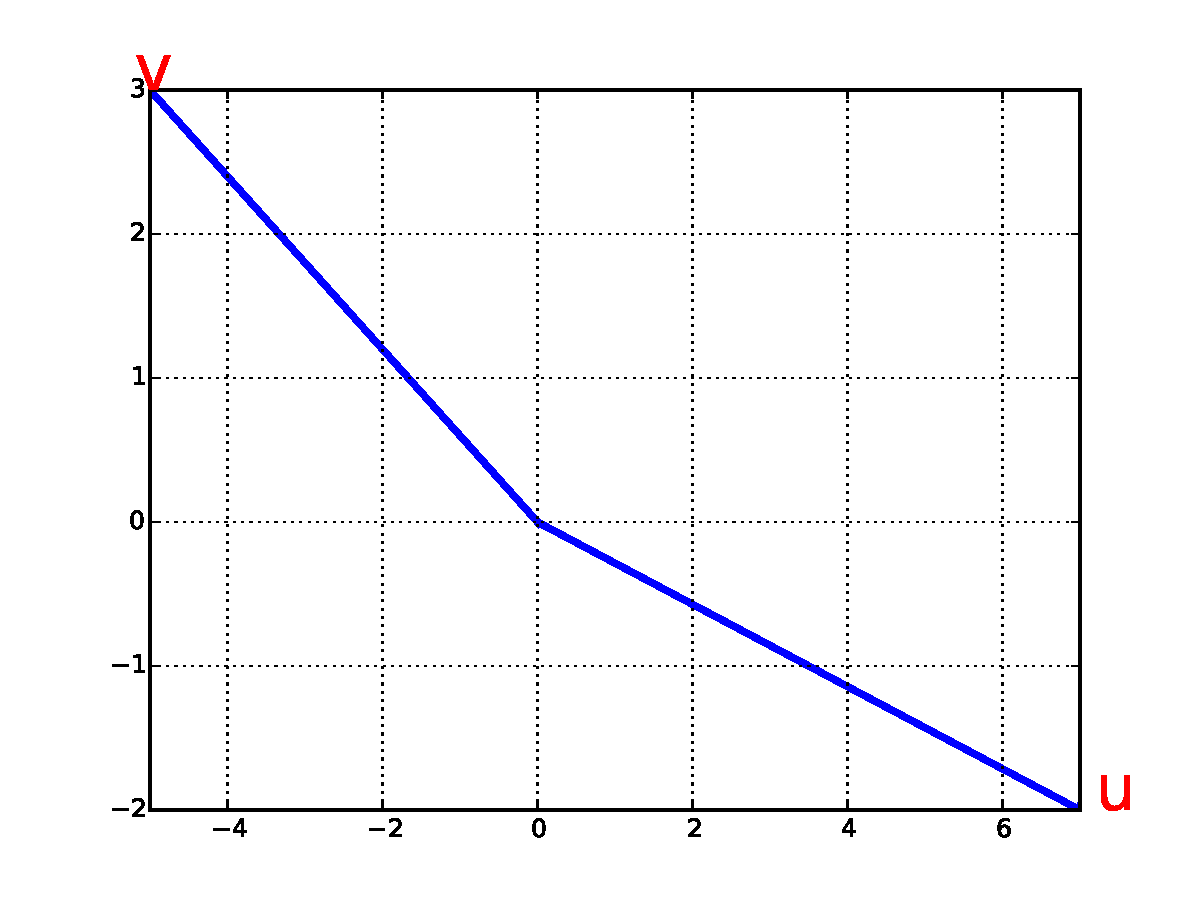
\includegraphics[width=\linewidth]{figs/ex2_1_6.pdf}

\begin{verbatim}
u= Matrix(2, 1, [7, -2])
v= Matrix(2, 1, [-5, 3])

plt.text(float(u[0])+0.2, float(u[1]), 'u', fontsize= 30, color= 'r')
plt.text(float(v[0])-0.2, float(v[1]), 'v', fontsize= 30, color= 'r')
plt.arrow(0, 0, float(u[0]), float(u[1]), lw= 3, color= 'b', head_width=0.05)
plt.arrow(0, 0, float(v[0]), float(v[1]), lw= 3, color= 'b', head_width=0.05)
plt.xlim((-5, 7))
plt.ylim((-2, 3))
plt.grid()
plt.savefig('figs/ex2_1_6.pdf')
plt.close()

(u + v).norm() # sqrt(5)
(u - v).norm() # 13
\end{verbatim}


\subsection{Further Properties of Vectors}
% ========================================

\subsubsection{Exercise 2.2.1}

Find the angle between vectors. The angle is

\begin{equation}\label{eq:uv_angle}
\theta = \arccos(\frac{\mathbf{u} \cdot \mathbf{v}}
{\|\mathbf{u}\| \cdot \|\mathbf{v}\|})
\end{equation}

In \sympy

\begin{verbatim}
def uv_angle(u, v):
    theta= acos(u.dot(v) / (u.norm() * v.norm()))
    return theta
\end{verbatim}

\begin{verbatim}
u= Matrix([1, 1])
v= Matrix([0, 1])
uv_angle(u, v) # pi/4

# As degree:
uv_angle(u, v) * 180/pi # 45

u= Matrix([-1, 2, 3])
v= Matrix([sqrt(2), 1/sqrt(2), -1])
uv_angle(u, v) * 180/pi # ~115 deg
\end{verbatim}

\subsubsection{Exercise 2.2.4}
% ----------------------------
Determine the vector of $k$ so that the vectors are orthogonal to each other.

We want to set the angle between vector equal to 0, \emph{i.e.} Eq. \ref{eq:uv_angle} = 0.

\begin{verbatim}
k= symbols('k', real= True)
u= Matrix([-1, 5, k])
v= Matrix([-3, 2, 7])

eq= Eq(u.dot(v) / (u.norm() * v.norm()) , cos(pi/2))
sol= solve(eq)

# Check
u.subs(k, sol[0]).dot(v) == 0 # True
\end{verbatim}

\subsubsection{Exercise 2.2.6}
% ----------------------------

A vector is normalized by dividing it by its norm. A normalized vector is called
\textbf{unit vector}. In \sympy normlaize with:

\begin{verbatim}
def norm_u(u):
    return u / u.norm()
\end{verbatim}

Determine the value of $k$ so that $\mathbf{\hat{u}} = (1/\sqrt{2}\ 1/2\ k)^T$.

For \textbf{u} to be unit vector, its norm must equal 1. So $\mathbf{\|u\|} = \sqrt{\left\lvert{k}\right\rvert^{2} + 0.75} = 1$.
Solved for $k= \pm 1/2$.

\begin{verbatim}
u= Matrix([1/sqrt(2), 1/2, k])
eq= Eq(u.norm(), 1)
ksol= solve(eq) # [-0.5, 0.5]
\end{verbatim}

\subsubsection{Exercise 2.2.12: Support vector machine}
% -----------------------------------------------------

Find the shortest distance between the vector \textbf{u} and the corresponding
hyperplane. The hyperplane is defined as $\mathbf{v \cdot x} + c = 0$ where
\textbf{v} is a vector of coefficents for the variables in vector \textbf{x} and
$c$ is a constant term. The vector \textbf{u} might represent a data point in
$n$-dimensions.

Remember that an equation in the usual form
$$ax + by +cz + k = 0$$
can be represented in matrix form as
$$ax + by +cz + k
= \left[\begin{matrix}a\\b\\c\end{matrix}\right] \cdot \left[\begin{matrix}x\\y\\z\end{matrix}\right] + k
= \mathbf{v} \cdot \mathbf{x} + k
= 0$$

The shortest distance between \textbf{u} and hyerplane is given by

\begin{equation}\label{eq:ex2_2_12_svm}
d_{shortest} = \frac{|\mathbf{u \cdot v} + c|}{\|\mathbf{v}\|}
\end{equation}

Given \textcolor{red}{$\mathbf{u} = (1\ 1)^T$} and hyperplane \textcolor{blue}{$y= x + 1$}, find the shortes
distance. For this we need to extract the vector of coefficents \textbf{v} from $y= x + 1$, which for convenience can be
re-arranged as $x - y + 1 = 0$.
The coeffients \textbf{v} are $\left[\begin{matrix}1\ \mathit{x} \\ -1\ \mathit{y} \end{matrix}\right]$.

Putting it all together:

\begin{equation}
d_{shortest} = \frac{
    |\left[\begin{matrix}1\\1\end{matrix}\right] \cdot \left[\begin{matrix}1\\-1\end{matrix}\right] + 1|
}{
    \|\left[\begin{matrix}1\\-1\end{matrix}\right]\|
} = \frac{\sqrt{2}}{2} \approx 0.707
\end{equation}

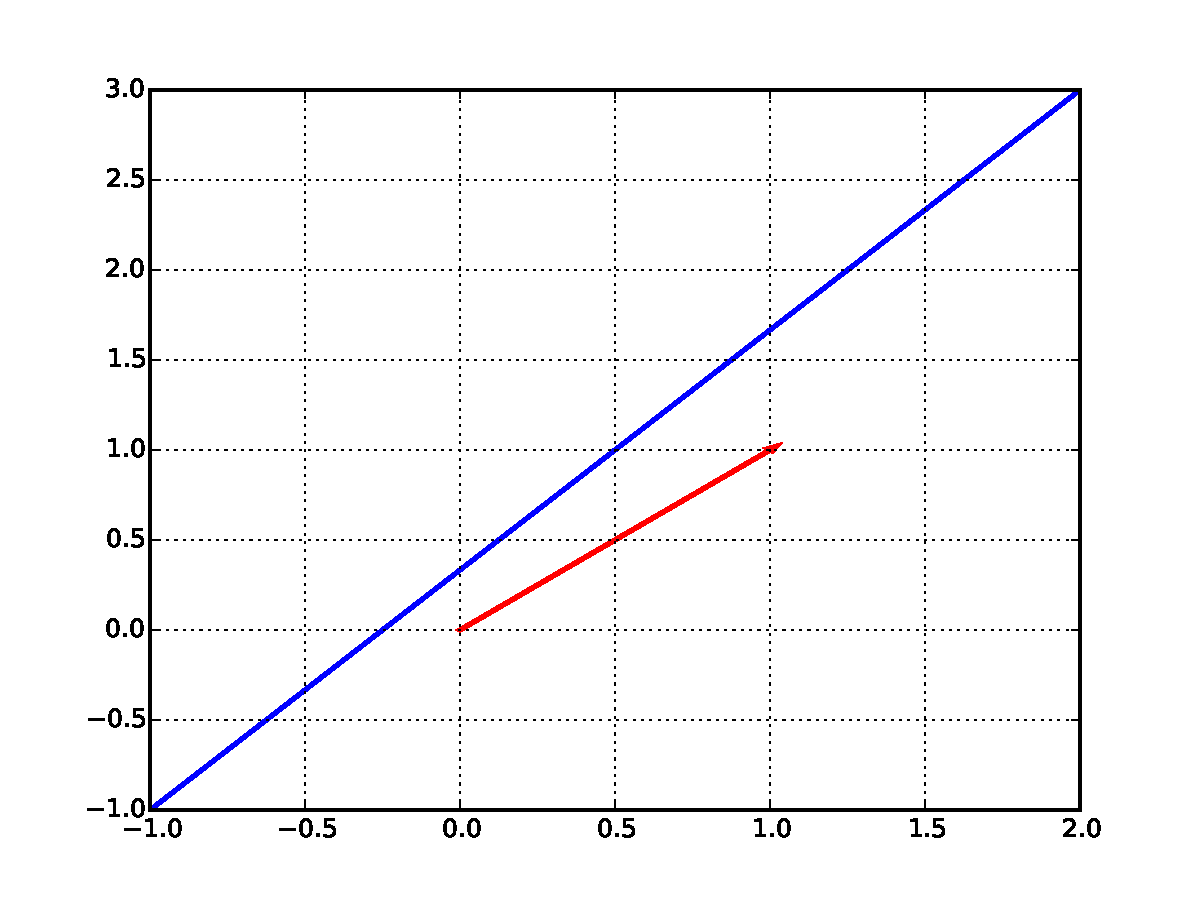
\includegraphics[width=0.75\linewidth]{figs/ex2_2_12_svm.pdf}

\begin{verbatim}
u= Matrix([1, 1])
hyp= Eq(x + 1, y)

# 1. Re-arrange hyp to have x + y + c= 0
hyp2= Eq(hyp.lhs - hyp.rhs)

# 2. Re-arrange in matrix form
cfdict= hyp2.lhs.as_expr().as_coefficients_dict()
v= Matrix([cfdict[x], cfdict[y]])
c= cfdict[numbers.One()]
d_shortest= abs(u.dot(v) + c) / v.norm()
\end{verbatim}

Plotted with:

\begin{verbatim}
plt.plot([-1, 2], [hyp.lhs.subs(x, -2), hyp.lhs.subs(x, 2)], 'b-', lw= 2)
plt.arrow(0, 0, float(u[0]), float(u[1]), lw= 2, color= 'red')
plt.grid()
plt.xlim([-0.5, 1.5])
plt.ylim([-0.5, 1.5])
plt.savefig('figs/ex2_2_12_svm.pdf')
plt.close()
\end{verbatim}

\subsubsection{Exercise 2.2.12d}
% ------------------------------

For $\mathbf{u} = \left[\begin{matrix}1\\2\\3\\4\end{matrix}\right]$ and
$x + 2y + z + w = 10$. We have

$$
d_{shortest}
= \frac{|\mathbf{u} \cdot \mathbf{v} + c|}{\|\mathbf{v}\|}
= \frac{|\left[\begin{matrix}1\\2\\3\\4\end{matrix}\right] \cdot \left[\begin{matrix}1\\2\\1\\1\end{matrix}\right] - 10|}{\|\left[\begin{matrix}1\\2\\1\\1\end{matrix}\right]\|}
= \frac{2 \sqrt{7}}{7}
\approx 0.76
$$

\begin{verbatim}
x,y,z,w = symbols('x y z w')
u = Matrix([1,2,3,4])
hyp= Eq(x + 2*y + z + w, 10)

hyp= hyp.lhs - hyp.rhs
v= [hyp.as_coefficients_dict()[t] for t in (x, y, z, w)]
v= Matrix(v)
c= hyp.as_coefficients_dict()[numbers.One()]

d_shortest= abs(u.dot(v) + c) / v.norm()
\end{verbatim}

\subsection{Linear Independence}
% ==============================

\subsubsection{Exercise 2.3.1}
% ----------------------------

Determine which vectors in $\mathbb{R}^2$ are \textbf{linearly dependent}.

The linear combination of vectors \textbf{u} and \textbf{v} is

\begin{equation}\label{eq:ex2_3_1}
k\mathbf{u} + c\mathbf{v} = \mathbf{O}
\end{equation}

Or more verbose:

\begin{equation}\label{eq:ex2_3_1_II}
k \left[\begin{matrix}x_1\\x_2\end{matrix}\right] +
c \left[\begin{matrix}y_1\\y_2\end{matrix}\right] =
\left[\begin{matrix}0\\0\end{matrix}\right]
\end{equation}

Where $k$ and $c$ are scalars (unknown coefficients). If \ref{eq:ex2_3_1} is
satisfied for $k \neq 0$ or $c \neq 0$ then \textbf{u} and \textbf{v} are
linearly dependent. Which means that \textbf{u} can be expressed as \textbf{v} times
a scalar, or vice versa.

Expressed as a system of equations, \ref{eq:ex2_3_1_II} becomes:

\begin{equation}
\begin{matrix}
kx_1 + cy_1 = 0 \\
kx_2 + cy_2 = 0
\end{matrix}
\end{equation}

Now solve this system and check whether $k=0$ and $c=0$ are the only solutions.

For $\mathbf{u} = \left[\begin{matrix}6\\10\end{matrix}\right]$  and
$\mathbf{v} = \left[\begin{matrix}-3\\-5\end{matrix}\right]$ we have:

$$
k \left[\begin{matrix}6\\10\end{matrix}\right] + c \left[\begin{matrix}-3\\-5\end{matrix}\right] = \left[\begin{matrix}0\\0\end{matrix}\right]
$$

re-arranged as a system

$$
\begin{matrix}6 k - 3 c = 0\\10 k - 5 c = 0\end{matrix}
$$

With solutions $\begin{bmatrix}\begin{Bmatrix}k : \frac{c}{2}\end{Bmatrix}, & \begin{Bmatrix}c : 2 k\end{Bmatrix}\end{bmatrix}$
which hold for $c$ and $k$ different from 0.

\begin{verbatim}
u= Matrix([6, 10])
v= Matrix([-3, -5])
eq1= Eq(k * u[0] + c * v[0], 0)
eq2= Eq(k * u[1] + c * v[1], 0)

csol= solve([eq1, eq2], c)
ksol= solve([eq1, eq2], k)
\end{verbatim}

Note that the conclusion of linear dependence can be reached by looking at the
rank of the matrix $\mathbf{A}= \left[\begin{matrix}\mathbf{u} & \mathbf{v}\end{matrix}\right]$.
In fact, $rank(\mathbf{A})$ is less than 2.

$$
\mathbf{A} = \left[\begin{matrix}\mathbf{u} & \mathbf{v}\end{matrix}\right]
= \left[\begin{matrix}6 & -3\\10 & -5\end{matrix}\right]
$$

with $rank(\mathbf{A}) = 1$. Note that trying to solve \textbf{A} results in
\sympy error \textcolor{red}{\texttt{ValueError: Matrix det == 0; not invertible.}}

In addition, note that the RREF has only one leading row:

$$
\mathbf{A_{rref}} = \begin{pmatrix}\left[\begin{matrix}1 & - \frac{1}{2} & 0\\0 & 0 & 0\end{matrix}\right], & \begin{bmatrix}0\end{bmatrix}\end{pmatrix}
$$

\begin{verbatim}
A= v.col_insert(0, u)
A_rank= A.rank() # 1

try:
    A.solve(Matrix([0, 0])) # Matrix det == 0; not invertible.
except ValueError, e:
    print e
    
A_rref= A.col_insert(2, Matrix([0,0])).rref()
\end{verbatim}

Unit vectors $\mathbf{e_1} = \left[\begin{matrix}1\\0\end{matrix}\right]$ and
$\mathbf{e_2} = \left[\begin{matrix}0\\1\end{matrix}\right]$ are linearly independent.
Note that $rank(\mathbf{A}) = N_{dimensions} = 2$ and the RREF is complete

$$
\mathbf{A_{rref}} = \begin{pmatrix}\left[\begin{matrix}1 & 0 & 0\\0 & 1 & 0\end{matrix}\right], & \begin{bmatrix}0, & 1\end{bmatrix}\end{pmatrix}
$$

\begin{verbatim}
k, c= symbols('k c')
e1= Matrix([1, 0])
e2= Matrix([0, 1])

eq1= Eq(k * e1[0] + c * e1[1], 0)
eq2= Eq(k * e2[0] + c * e2[1], 0)

solve([eq1, eq2]) # {c: 0, k: 0}

# Also
A= e2.col_insert(0, e1)
A_rank= A.rank() # 2

A_rref= A.col_insert(2, Matrix([0,0])).rref()
\end{verbatim}

\subsubsection{Exercise 2.3.12 - \textit{incomplete}}
% ---------------------------------------------------

Determine the value of $t$ in the \textbf{linearly independent} vectors

$$
\mathbf{u} = \left[\begin{matrix}t\\1\\1\end{matrix}\right],
\mathbf{v} = \left[\begin{matrix}-1\\t\\1\end{matrix}\right],
\mathbf{w} = \left[\begin{matrix}1\\1\\t\end{matrix}\right],
$$

The RREF of the augmented matrix is:

$$
\mathbf{A_{rref} = \begin{pmatrix}\left[\begin{matrix}1 & 0 & 0 & 0\\0 & 1 & 0 & 0\\0 & 0 & 1 & 0\end{matrix}\right], & \begin{bmatrix}0, & 1, & 2\end{bmatrix}\end{pmatrix}}
$$

which implies that either the coefficients $k_1 = k_2 = k_3 = 0$ or $t$

\begin{verbatim}
t, k1, k2, k3= symbols('t k1 k2 k3', real= True)

u= Matrix([ t, 1, 1]) # k1
v= Matrix([-1, t, 1]) # k2
w= Matrix([ 1, 1, t]) # k3

eq1= Eq(k1*t - k2   + k3,   0)
eq2= Eq(k1   + k2*t + k3,   0)
eq3= Eq(k1   + k2   + k3*t, 0)

A= w.col_insert(0, v).col_insert(0, u)
Au= Matrix([0,0,0]).col_insert(0, A)
A_rref= Au.rref()
\end{verbatim}

\subsection{Basis and Spanning Set}
% =================================

\subsubsection{Example 2.17}
% ----------------------------

Determine whether the vectors $\mathbf{u} = \left[\begin{matrix}1\\2\end{matrix}\right]$
and $\mathbf{v} = \left[\begin{matrix}-1\\1\end{matrix}\right]$ \textbf{span} $\mathbb{R}^2$.
In other words, the question is whether with the axis \textbf{u} and \textbf{v}
we can draw any vector in $\mathbb{R}^2$. In other words again, can any vector in
$\mathbb{R}^2$ be defined as a \emph{\textbf{linear combination}} of \textbf{u} and \textbf{v}?

So let's take a generic vector in $\mathbb{R}^2$ $\mathbf{w} = \left[\begin{matrix}a\\b\end{matrix}\right]$
and see if the equation

\begin{equation}\label{eq:example_2_17}
\mathbf{w} = k\mathbf{u}  + c\mathbf{v}
\end{equation}

can be solved to find the coefficients \textbf{k} and \textbf{c}.
If the answer is yes, than the generc vector \textbf{w} can be defined in terms
of \textbf{u} and \textbf{v} given appropriate coefficients $k$ and $c$ respectively.

To solve \ref{eq:example_2_17} build the augmented matrix

$$\mathbf{A} =
\left[\begin{matrix}1 & -1 & a\\2 & 1 & b\end{matrix}\right]$$,

put in RREF and see if the RREF is complete. In this case

$$\mathbf{A_{rref}} = \left[\begin{matrix}1 & 0 & \frac{a}{3} + \frac{b}{3}\\0 & 1 & - \frac{2 a}{3} + \frac{b}{3}\end{matrix}\right]$$

The coefficients \textbf{k} and \textbf{c} are given as the last column

\begin{equation}\label{eq:example_2_17_ii}
k, c= \left[\begin{matrix}\frac{a}{3} + \frac{b}{3}\\- \frac{2 a}{3} + \frac{b}{3}\end{matrix}\right]
\end{equation}

Here $a$ and $b$ can be thought as increments on the $x$ and $y$ axis.

For example, how do we express the vector $\mathbf{g} = \left[\begin{matrix}3\\2\end{matrix}\right]$
in the \textbf{spanning set} \textbf{u} and \textbf{v}? By substituting in \ref{eq:example_2_17_ii}
3 for $a$ and 2 for $b$ we get the coefficients $k= 5/3$ and $c = -4/3$. Therefore

\begin{align}
\mathbf{g} = \left[\begin{matrix}3\\2\end{matrix}\right]
= k\mathbf{u} + c\mathbf{v} \\
= \left[\begin{matrix}\frac{a}{3} + \frac{b}{3}\end{matrix}\right] \mathbf{u} + \left[\begin{matrix}- \frac{2 a}{3} + \frac{b}{3} \mathbf{v}\end{matrix}\right] \\
= \left[\begin{matrix}\frac{3}{3} + \frac{2}{3}\end{matrix}\right] \mathbf{u} + \left[\begin{matrix}- \frac{2 \cdot 3}{3} + \frac{2}{3} \mathbf{v}\end{matrix}\right] \\
= 5/3 \mathbf{u} + -4/3 \mathbf{v} \\
= \left[\begin{matrix}3\\2\end{matrix}\right]
\end{align}

\begin{verbatim}
a,b,c,k= symbols('a b c k')

u= Matrix([1, 2])
v= Matrix([-1, 1])
w= Matrix([a, b])

A= w.col_insert(0, v).col_insert(0, u)
A_rref= A.rref()

# Coefficients
k, c= A_rref[0].col(- 1)

# Or maybe easier using M.solve(const)
A= v.col_insert(0, u)
k, c= A.solve(w)

## Represent g in spanning set (u, v)
g= Matrix([3, 2])
k2= k.subs({a:g[0], b:g[1]})
c2= c.subs({a:g[0], b:g[1]})
g2= k2 * u + c2 * v
\end{verbatim}

\subsubsection{Exercise 2.4.1}
% ----------------------------

Determine whether the following vectors span $\mathbb{R}^2$

\begin{verbatim}
# Generic vector
w= Matrix([a, b])

e1= Matrix([1, 0])
e2= Matrix([0, 1])

A= w.col_insert(0, e2).col_insert(0, e1)
\end{verbatim}

For unit vectors $\mathbf{e_1}$ and $\mathbf{e_2}$ the answer is yes with
coefficient a and b from RREF

$$
\mathbf{A_{rref}} = \left[\begin{matrix}1 & 0 & a\\0 & 1 & b\end{matrix}\right]
$$

These vectors do not form a spanning set as a generic vector \textbf{w} cannot be formed
by linear combination. The augmented matrix cannot be in RREF:

$$
\mathbf{A_{rref}} = \left[\begin{matrix}1 & - \frac{1}{2} & 0\\0 & 0 & 1\end{matrix}\right]
$$

Trying to solve the augmented matrix \textcolor{red}{\texttt{ValueError: Matrix det == 0; not invertible.}}

$$
\mathbf{A} = \left[\begin{matrix}2 & -1 & a\\2 & -1 & b\end{matrix}\right]
$$

Results in 

\begin{verbatim}
u= Matrix([2, 2])
v= Matrix([-1, -1])
A= w.col_insert(0, v).col_insert(0, u)
A.rref() # Not in RREF

# Indeed:
A= v.col_insert(0, u)
A.solve(w) # ValueError: Matrix det == 0; not invertible.
\end{verbatim}

\subsubsection{Exercise 2.4.2}
% ----------------------------

Determine whether the following vectors span $\mathbb{R}^3$

\begin{verbatim}
u= Matrix([1, 2, 1])
v= Matrix([2, 4, 0])
w= Matrix([-2, -2, 3])
\end{verbatim}

So, let's define a generic vector in $\mathbb{R}^3$

\begin{verbatim}
a,b,c= symbols('a b c')
g= Matrix([a, b, c])
\end{verbatim}

and define \textbf{g} as a linear combination of \textbf{u, v, w}
\emph{i.e.}
$$ \mathbf{g}= k\mathbf{u} + j\textbf{v} + l\mathbf{w}$$

Can we solve these linear system to find the unknow $k, j, l$?

To answer, prepare the augmented matrix (not really necessary to prepare it though).
Note the use of \texttt{numpy.hstack} to column-bind vectors. Now try to solve it

\begin{verbatim}
A= Matrix(numpy.hstack((u, v, w, g)))
sol= A[:, :-1].solve(A[:, -1])
\end{verbatim}

The syntax to slice the matrix comes from \href{http://docs.scipy.org/doc/numpy/reference/arrays.indexing.html}{NumPy}:
\textcolor{blue}{\texttt{A[:, :-1]}} means get all rows with ':' (1st index) and all columns
excluding the last one with ':-1'.

Anyway, the solution exists and is

$$
k, j, l= \left[\begin{matrix}3 a - \frac{3 b}{2} + c\\- 2 a + \frac{5 b}{4} - \frac{c}{2}\\- a + \frac{b}{2}\end{matrix}\right]
$$

so \textbf{u, v, w} are spanning set of $\mathbb{R}^3$

\subsubsection{Exercise 2.4.3}
% ----------------------------

Determine whether the following vectors form a \textbf{\textit{basis}} for $\mathbb{R}^2$

\begin{verbatim}
u= Matrix([1, 2])
v= Matrix([0, 1])
\end{verbatim}

A \textbf{\textit{basis}} is a spanning set whose vectors are also linearly independent.
This means that a basis is the minimal set of vectors necessary to describe the
$\mathbb{R}^n$ space. Note that if the vectors span $\mathbb{R}^n$ than they are
linearly independent and \emph{vice versa}. So we need to check only one of the two
conditions.

In the case above we have linearl independence since:

$$
A = \left[\begin{matrix}u\\v\end{matrix}\right]
= \left[\begin{matrix}0 & 1\\1 & 2\end{matrix}\right]
$$

and a solution can be found:

$$
a, b= \left[\begin{matrix}- 2 a + b\\a\end{matrix}\right]
$$

\begin{verbatim}
A= Matrix(numpy.array((u, v)))
sol= A.solve(Matrix([a, b]))
A.rank() == A.rows # True (2)
A.det() != 0 # True
A.rref() 
\end{verbatim}

Note also that $rank(A) = 2$, \emph{i.e.} \textbf{A} is full rank and the RREF
is complete $\left[\begin{matrix}1 & 0\\0 & 1\end{matrix}\right]$

In this case, there is no linear independence and the vectors are not a basis:

\begin{verbatim}
u= Matrix([-2, -4])
v= Matrix([1, 2])
A= Matrix(numpy.array((u, v)))
sol= A.solve(Matrix([a, b]))  ## ValueError: Matrix det == 0; not invertible.
A.rank() == A.rows # False
A.det() == 0 # True
\end{verbatim}

\subsubsection{Exercise 2.4.4}
% ----------------------------

Do these vector form a basis for $\mathbb{R}^4$?

\begin{verbatim}
u= Matrix([1, 1, 1, 1])
v= Matrix([1, 1, 0, -1])
w= Matrix([-1, -2, -3, 4])
x= Matrix([2, 2, 2, 2])
A= Matrix(numpy.hstack([u, v, w, x]))
\end{verbatim}

No since they are not linearly independent. In fact u and x are multiple of each other.

\subsubsection{Exercise 2.4.5}
% ----------------------------

Is \textbf{b} in the space spanned by the columns of matrix \textbf{A}?

\begin{equation}
\mathbf{A} = \left[\begin{matrix}1 & 1 & 0\\2 & 5 & 0\\3 & 4 & 9\end{matrix}\right];
\mathbf{b} = \left[\begin{matrix}1\\3\\4\end{matrix}\right]
\end{equation}

To answer we want to know whether the columns of \textbf{A} can be linearly combined
to produce \textbf{b}. Can we found a vector \textbf{k} of coefficients for the
columns in \textbf{A} that produce \textbf{b}?
So we want ot see if we can solve $\mathbf{Ak} = \mathbf{b}$ \emph{w.r.t.} \textbf{k}.
\emph{I.e.} let's try to solve $\mathbf{k}= \mathbf{A}^{-1}\mathbf{b}$. We can solve it
for $\mathbf{k} = \left[\begin{matrix}\frac{2}{3}\\\frac{1}{3}\\\frac{2}{27}\end{matrix}\right]$.

We can also verify that $\mathbf{Ak} = \mathbf{b}$.

\begin{verbatim}
A= Matrix([[1, 1, 0], [2, 5, 0], [3, 4, 9]])
b= Matrix([1, 3, 4])

k= A.inv().dot(b)
# The same:
k= A.solve(b)

# Check back:
b == Matrix(A.dot(k))
\end{verbatim}

What about this case:

\begin{verbatim}
A= Matrix([[1, 2, 3],
           [4, 5, 6],
           [7, 8, 9]])
b= Matrix([1, 3, 4])
A.inv() ## ValueError: Matrix det == 0; not invertible.
A.solve(b) ## The same
\end{verbatim}

\texttt{ValueError: Matrix det == 0; not invertible}, in fact the columns of \textbf{A}
are not linearly independent we cannot find a vector of coefficients \textbf{k} 
to represent \textbf{b}.

\begin{verbatim}
\end{verbatim}

\subsubsection{Exercise 2.4.6}
% ----------------------------

Are these vectors a basis for $mathbb{R}^3$?

\begin{verbatim}
u= Matrix([5, 0, 0])
v= Matrix([0, 6, 0])
w= Matrix([0, 0, 7])
A= Matrix(numpy.hstack([u, v, w]))
A.solve(Matrix([a, b, c])) ## Solvable -> lin. indep. -> basis
\end{verbatim}

What about:

\begin{verbatim}
alpha, beta, lamda= symbols('alpha beta lamda', real= True, nonzero= True)
u= Matrix([alpha, 0, 0])
v= Matrix([0, beta, 0])
w= Matrix([0, 0, lamda])
A= Matrix(numpy.hstack([u, v, w]))
A.solve(Matrix([a, b, c])) ## Solvable -> lin. indep. -> basis

# Also:
A.inv() # Ok
A.rank() == 3 # True
A.det() != 0 # True
\end{verbatim}

\section{3. General vector spaces}
% *********************************

\subsection{3.3 Linear independence and basis}
% ============================================

\subsubsection{Exercise 3.3.1}
%-----------------------------

Are the \textbf{A} and \textbf{B} matrices linearly independent?

They are independent if there is no scalar that can multiply one matrix to return the other. So if there
is a solution for $x$  to $Ax = B$, \textbf{A} and \textbf{B} are linearly dependent.

For
$$
\mathbf{A} = \left[\begin{matrix}1 & 1\\1 & 1\end{matrix}\right];
\mathbf{B} = \left[\begin{matrix}2 & 2\\2 & 2\end{matrix}\right];
\mathbf{A}x = \mathbf{B} = \left[\begin{matrix}1 & 1\\1 & 1\end{matrix}\right]x = \left[\begin{matrix}2 & 2\\2 & 2\end{matrix}\right]
$$

$x= 2$ can solve the equation and transform \textbf{A} into \textbf{B} hence the
two matrices are dependent.

\begin{verbatim}
A= Matrix(2, 2, [1,1,1,1])
B= Matrix(2, 2, [2,2,2,2])
solve(Eq(x*A, B), x) # {x: 2} dependent.
\end{verbatim}

The equation $\left[\begin{matrix}1 & 2 \\3  & 4 \end{matrix}\right]x = \left[\begin{matrix}2 & 2\\2 & 2\end{matrix}\right]$
has no solution for $x$, so \textbf{A} and \textbf{B} are independent.

\begin{verbatim}
A= Matrix(2, 2, [1, 2,
                 3, 4])
B= Matrix(2, 2, [2, 2,
                 2, 2])
Eq(A*x, B)
\end{verbatim}

\subsubsection{Example 3.15}
%---------------------------

Given three vectors in the space of continuous functions:

$$
\mathbf{u}= cos(x) \quad
\mathbf{v}= sin(x) \quad
\mathbf{w}= 2
$$

We show they are \textbf{linearly independent} by solving:

$$
k_1\mathbf{u} + k_2\mathbf{v} + k_1\mathbf{w}= 0
$$

For $k_1, k_2, k_3$. If the only solution is for $k_1 = k_2 = k_3 = 0$, the functions
are linearly independent.

To find solutions for $k_1, k_2, k_3$ we need a system of three equations.
In each equation $x$ is replaced by a convenient value which makes the arithmetic
easier. In this case we could use $x= 0, x= \pi, x= \pi/2$. Here we replace $x$ with
a generic constant $c_1, c_2, c_3$ since the dirty job of solving the system is left
to \sympy.

$$
\left[\begin{matrix}
k_{1} \mathbf{u} + k_{2} \mathbf{v} + k_3 \mathbf{w} \\
k_{1} \mathbf{u} + k_{2} \mathbf{v} + k_3 \mathbf{w} \\
k_{1} \mathbf{u} + k_{2} \mathbf{v} + k_3 \mathbf{w} \\
\end{matrix}\right]
=
\left[\begin{matrix}
k_{1} \cos{\left (c_{1} \right )} + k_{2} \sin{\left (c_{1} \right )} + 2 k_{3} \\
k_{1} \cos{\left (c_{2} \right )} + k_{2} \sin{\left (c_{2} \right )} + 2 k_{3} \\
k_{1} \cos{\left (c_{3} \right )} + k_{2} \sin{\left (c_{3} \right )} + 2 k_{3}
\end{matrix}\right]
=
\left[\begin{matrix}
0 \\
0 \\
0 \\
\end{matrix}\right]
$$

\begin{verbatim}
x,k1,k2,k3= symbols('x k1:4', real= True)
u= cos(x)
v= sin(x)
w= 2

eq= Eq(k1*u + k2*v + k3*w, 0)
c1, c2, c3= symbols('c1:4', real= True)
eq1= eq.subs(x, c1)
eq2= eq.subs(x, c2)
eq3= eq.subs(x, c3)
solve([eq1, eq2, eq3], [k1, k2, k3])
\end{verbatim}

Given

$$
\mathbf{f} = \cos^{2}{\left (x \right )}, \quad
\mathbf{g}= \sin^{2}{\left (x \right )}, \quad
\mathbf{h}= 5
$$

The linear combination

$$
k_{1} \mathbf{f} + k_{2} \mathbf{g} + k_3 \mathbf{h} = 
k_{1} \cos^{2}{\left (x \right )} + k_{2} \sin^{2}{\left (x \right )} + 5 k_{3} = 0
$$

is solved with the system

$$
\left[\begin{matrix}
k_{1} \cos^{2}{\left (c_{1} \right )} + k_{2} \sin^{2}{\left (c_{1} \right )} + 5 k_{3} = 0 \\
k_{1} \cos^{2}{\left (c_{2} \right )} + k_{2} \sin^{2}{\left (c_{2} \right )} + 5 k_{3} = 0 \\
k_{1} \cos^{2}{\left (c_{3} \right )} + k_{2} \sin^{2}{\left (c_{3} \right )} + 5 k_{3} = 0
\end{matrix}\right]
$$

where $\left \{ k_{1} : - 5 k_{3}, \quad k_{2} : - 5 k_{3}\right \}$. Since $k_1,
k_2, k_3$ are not all equal to zero, the functions are linearly dependent. 

\begin{verbatim}
f= cos(x)**2
g= sin(x)**2
h= 5

def testLinearIndep(f, g, h):
    ## Linear combination
    k1, k2, k3= symbols('k1:4')
    eq= Eq(k1*f + k2*g + k3*h, 0)
    
    ## Linear system:
    c1, c2, c3= symbols('c1:4')
    eq1= eq.subs(x, c1)
    eq2= eq.subs(x, c2)
    eq3= eq.subs(x, c3)
    
    ## Solutions to linear system
    M= Matrix(3, 1, [eq1, eq2, eq3])
    sols= solve(M, [k1, k2, k3])
    return sols
\end{verbatim}

It can be attcked using Wronskian determinant \textbf{W}. If $\mathbf{W} \neq 0$ 
than the functions are linearly independent. However $\mathbf{W} = 0$ does not
necessarily mean dependence.

\begin{verbatim}
k1, k2, k3= symbols('k1:4')
f= cos(x)**2
g= sin(x)**2
h= 5

def wronskian(f, g, h):
    W= Matrix([[f, g, h],
            [diff(f, x), diff(g, x), diff(h, x)],
            [diff(f, x, 2), diff(g, x, 2), diff(h, x, 2)]])
    return W.det()
    
wronskian(f, g, h) # == 0 => *Suggests* lin. dep.
\end{verbatim}

\subsubsection{Exercise 3.3.3c}
% -----------------------------
\begin{verbatim}
f= 1
g= x
h= x**2
testLinearIndep(f, g, h) #  {k1: 0, k2: 0, k3: 0} => Lin. Indep.
wronskian(f, g, h) # == 2 -> Lin. Indep.
\end{verbatim}

\subsubsection{Exercise 3.3.3d}
% -----------------------------

In this case, the Wronskian appears to be non-zero:

$$
\mathbf{W}= - 3 \sin^{2}{\left (x \right )} \sin{\left (2 x \right )}
\cos{\left (x \right )} - 6 \sin{\left (x \right )} \cos^{2}{\left (x \right )}
\cos{\left (2 x \right )} + 3 \sin{\left (2 x \right )} \cos^{3}{\left (x \right )}
$$

Although it seems to be very close to 0 for any value of $x$.

\begin{verbatim}
f= sin(2*x)
g= sin(x) * cos(x)
h= cos(x)
testLinearIndep(f, g, h) # {k1:-k2/2, k3: 0} => Lin dep.
w= wronskian(f, g, h) # \neq 0. Why?

## Wronskian close to but not zero:
max([float(w.subs(x, c/100)) for c in range(-200*pi, 200*pi)]) # 6.66e-16
\end{verbatim}

\subsubsection{Exercise 3.3.3e}
% -----------------------------

\begin{verbatim}
f= exp(x) * sin(2*x)
g= exp(x) * sin(x)* cos(x)
h= exp(x) * cos(x)
testLinearIndep(f, g, h) # {k1:-k2/2, k3: 0} => Lin dep.
w= wronskian(f, g, h)
max([float(w.subs(x, c/100)) for c in range(-200*pi, 200*pi)]) # 3.818e-08
\end{verbatim}

\subsubsection{Exercise 3.3.3f}
% -----------------------------
\begin{verbatim}
f= 1
g= exp(x)
h= exp(-x)
testLinearIndep(f, g, h) # k1 = k2 = k3 = 0 # Lin. Indep.
wronskian(f, g, h)       # wronskian= 2
\end{verbatim}

\subsubsection{Exercise 3.3.3g}
% -----------------------------

\begin{verbatim}
f= exp(x)
g= exp(2*x)
h= exp(3*x)
testLinearIndep(f, g, h) # k1 = k2 = k3 = 0 # Lin. Indep.
wronskian(f, g, h)       # wronskian == 2*exp(6*x) != 0
\end{verbatim}

\subsubsection{Exercise 3.3.4}
% ----------------------------

Same as exercise 

\begin{verbatim}
f= sin(x)
g= sin(3*x)
h= sin(5*x)
testLinearIndep(f, g, h) # k1 = k2 = k3 = 0 # Lin. Indep.
w= wronskian(f, g, h)  # !=0
\end{verbatim}

\subsubsection{Exercise 3.3.4}
% ----------------------------

Show that the following matrices are a \textbf{basis} for $M_{22}$, the vector space of
2 by 2 matrices.

$$
\mathbf{A}= \left[\begin{matrix}1 & 0\\0 & 0\end{matrix}\right], \quad
\mathbf{B}= \left[\begin{matrix}0 & 1\\0 & 0\end{matrix}\right], \quad
\mathbf{C}= \left[\begin{matrix}0 & 0\\1 & 0\end{matrix}\right], \quad
\mathbf{D}= \left[\begin{matrix}0 & 0\\0 & 1\end{matrix}\right]
$$

The following conditions must satisfied:

\begin{enumerate}
\item \textbf{Span}: Can any vector in $M_{22}$ be generated with \textbf{A, B, C, D}?
\item \textbf{Linear independence}: Are \textbf{A, B, C, D} linearly independent?
\end{enumerate}

To see if \textbf{A, B, C, D} \textbf{span} $M_{22}$ we generate a generic matrix
$\mathbf{M}= \left[\begin{matrix}a & b\\c & d\end{matrix}\right]$ and then we
see if a linear combination of \textbf{A, B, C, D} can produce \textbf{M}:
$$
k_1\mathbf{A} + k_2\mathbf{B} + k_3\mathbf{C} + k_4\mathbf{D} = \mathbf{M}
$$
Yes, we can combine \textbf{A, B, C, D} and produce \textbf{M} by setting
$\left \{ a : k_{1}, \quad b : k_{2}, \quad c : k_{3}, \quad d : k_{4}\right \}$

Are \textbf{A, B, C, D} also linearly independent? In other words is the
linear combination

$$
k_1\mathbf{A} + k_2\mathbf{B} + k_3\mathbf{C} + k_4\mathbf{D} = \mathbf{O}
$$
satisifed for values of $k$s other than $k_1=k_2=k_3=k_4=0$? No, as show in the code.

\begin{verbatim}
A= Matrix(2, 2, [1, 0, 0, 0])
B= Matrix(2, 2, [0, 1, 0, 0])
C= Matrix(2, 2, [0, 0, 1, 0])
D= Matrix(2, 2, [0, 0, 0, 1])

## Span
a,b,c,d= symbols('a b c d')
k1, k2, k3, k4= symbols('k1:5')
M= Matrix(2, 2, [a, b, c, d])
solve(Eq(k1*A + k2*B + k3*C + k4*D, M)) # {a: k1, b: k2, c: k3, d: k4}

## Linear independence
eq= Eq(k1*A + k2*B + k3*C + k4*D, zeros(2,2))
solve(eq) # {k1: 0, k2: 0, k3: 0, k4: 0}
\end{verbatim}

\subsubsection{Exercise 3.3.6}
% ----------------------------

Check whether the three polynomials $p, q, r$ form a basis for the vector space of
the polynomials of degree $\leq 2$.

\begin{enumerate}
\item \textbf{Span}: Take a general polynomial $y$ of degree 2 and see if the linear combination
of the $p, q, r$ can produce $y$
\item \textbf{Linear independence}: Check whether $p, q, r$ are linearly independent.
\end{enumerate}

$p, q, r$ do span $P^2$ by setting
$\left \{ k_{1} : a + b + c, \quad k_{2} : 2 a + b, \quad k_{3} : a\right \}$

$p, q, r$ are linearly independent since the only solution to
$k_{1} + k_{2} \left(t - 1\right) + k_{3} \left(t - 1\right)^{2} = 0$ is for
$\left \{ k_{1} : 0, \quad k_{2} : 0, \quad k_{3} : 0\right \}$.

\begin{verbatim}
t,a,b,c= symbols('t a b c')
k1, k2, k3= symbols('k1:4')
p= 1
q= t - 1
r= (t - 1)**2

## Span
y= a*t**2 + b*t + c
eq= Eq(k1*p + k2*q + k3*r, y)
solve(eq, [k1, k2, k3]) # {k1: a + b + c, k2: 2a + b, k3: a}

## Linear independence
eq= Eq(k1*p + k2*q + k3*r, 0)
solve(eq, [k1, k2, k3]) # {k1: 0, k2: 0, k3: 0}
\end{verbatim}

With $\mathbf{p, q, r}$ we can define any vector in $P^2$. For example, how can we
combine $\mathbf{p, q, r}$ to obtain $\mathbf{p_1} = t^{2} + 1$? \emph{I.e.}, what
coefficients $k_1, k_2, k_3$ do we need to assign to $\mathbf{p, q, r}$? We need to
solve the equation
$$
k_{1}\mathbf{p} + k_{2} \mathbf{q} + k_3\mathbf{r} = t^{2} + 1
$$
for $k_1, k_2, k_3$. It is solved with
$\left \{ k_{1} : 2, \quad k_{2} : 2, \quad k_{3} : 1\right \}$.

We can check this by substituting $k_1, k_2, k_3$ in $k_{1}\mathbf{p} + k_{2} \mathbf{q} + 5 \mathbf{r}$
and see that we obtain $t^2 + 1$.

\begin{verbatim}
p1= t**2 + 1
eq= Eq(k1*p + k2*q + k3*r, p1)
sols= solve(eq, [k1, k2, k3]) ## {k1: 2, k2: 2, k3: 1}

## Check sols return p1
pp= k1*p + k2*q + k3*r
pp.subs(sols).simplify()      ## => t**2 + 1
pp.subs(sols).simplify() - p1 ## => 0
\end{verbatim}

\subsubsection{Exercise 3.3.7}
% ----------------------------

$\mathbf{p}= 1, \quad \mathbf{q}= t^{2} - 2 t, \quad \mathbf{r}= 5 \left(t - 1\right)^{2}$ do not form a basis
for $P^2$ since the three polynomials are not linearly independent. In fact,
$k_{1}\mathbf{p} + k_{2} \mathbf{q} + 5 \mathbf{r} = 0$ is
solved for $\left \{ k_{1} : - 5 k_{3}, \quad k_{2} : - 5 k_{3}\right \}$

\begin{verbatim}
p= 1
q= t**2 - 2*t
r= 5*(t-1)**2

eq= Eq(k1*p + k2*q + k3*r, 0)
sols= solve(eq, [k1, k2, k3])
\end{verbatim}

\subsection{3.6 Linear systems revisted}
% ======================================

It is useful to keep in mind that all these statements are equivalent. If one is
true all the others are true. Given a $n$ by $n$ (square) matrix \textbf{A} we have:

\begin{itemize}
\item \textbf{A} is invertible.
\item \textbf{A} is full rank, \emph{i.e.} $rank(\mathbf{A}) = nrows(\mathbf{A}) = n$.
\item Rows in \textbf{A} are linearly independent.
\item Columns in \textbf{A} are linearly independent.
\item $nullity(\mathbf{A}) = 0$.
\item The \emph{nullspace} of \textbf{A} contains only the zero vector.
\end{itemize}

Given the system $\mathbf{Ax = O}$, the \textbf{\emph{nullspace}} is the set of
vectors that satisfies the system. The \emph{dimension} of the nullspace is called
\textbf{\emph{nullity}}. Consequently for a $n$ by $n$ matrix we have:

$$
rank(\mathbf{A}) + nullspace(\mathbf{A}) = n
$$

\subsubsection{Exercise 3.6.1}
%-----------------------------

Nullspace of 2 by 2 unit matrix $\left[\begin{matrix}1 & 0\\0 & 1\end{matrix}\right]$
is the zero vector since this is the only solution to $\mathbf{Av = O}$.

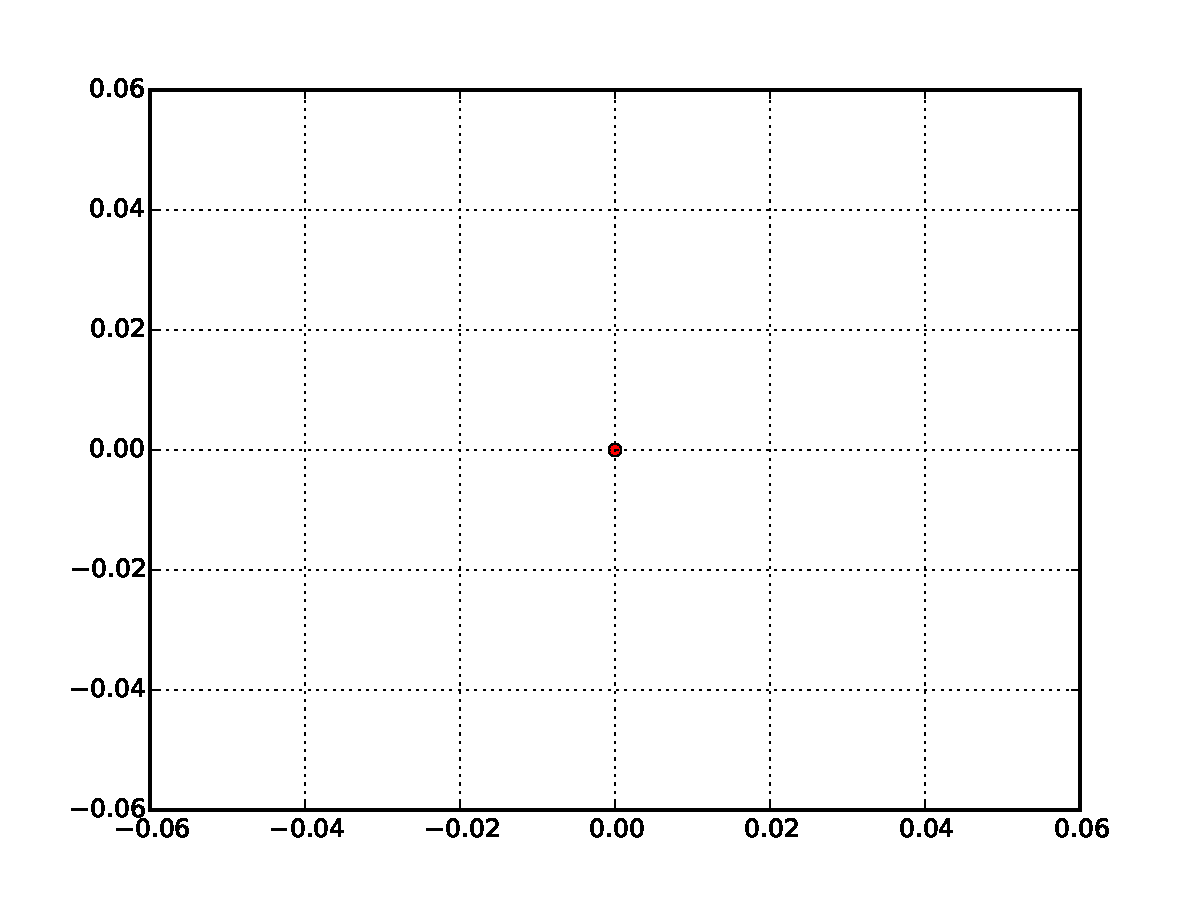
\includegraphics[width=0.7\linewidth]{figs/ex3_6_1.pdf}

\begin{verbatim}
x,y= symbols('x,y')
v= Matrix([x, y])
A= eye(2)

sols= solve(Eq(A*v, Matrix([0, 0])))[0] ## [{x: 0, y: 0}]
A.nullspace() ## Empty. 

plt.plot(sols[x], sols[y], 'ro')
plt.grid()
plt.savefig('figs/ex3_6_1.pdf')
\end{verbatim}

For $\mathbf{A}= \left[\begin{matrix}1 & 2\\2 & 4\end{matrix}\right]$ we need to
solve $\left[\begin{matrix}x + 2 y\\2 x + 4 y\end{matrix}\right] = \left[\begin{matrix}0\\0\end{matrix}\right]$.
Solution is $\left \{ x : - 2 y\right \}$ or $\left[\begin{matrix}-2\\1\end{matrix}\right]$.
Graphically, the nullspace is the vector passing by $\left[\begin{matrix}-2\\1\end{matrix}\right]$
as shown here below. In fact any point sitting on this line will make $\mathbf{Av = O}$.
\emph{E.g.} with $\mathbf{v} = [2\ -1]^T$ we have $\left[\begin{matrix}1 & 2\\2 & 4\end{matrix}\right] \left[\begin{matrix}2\\-1\end{matrix}\right] =
\left[\begin{matrix}0\\0\end{matrix}\right]$

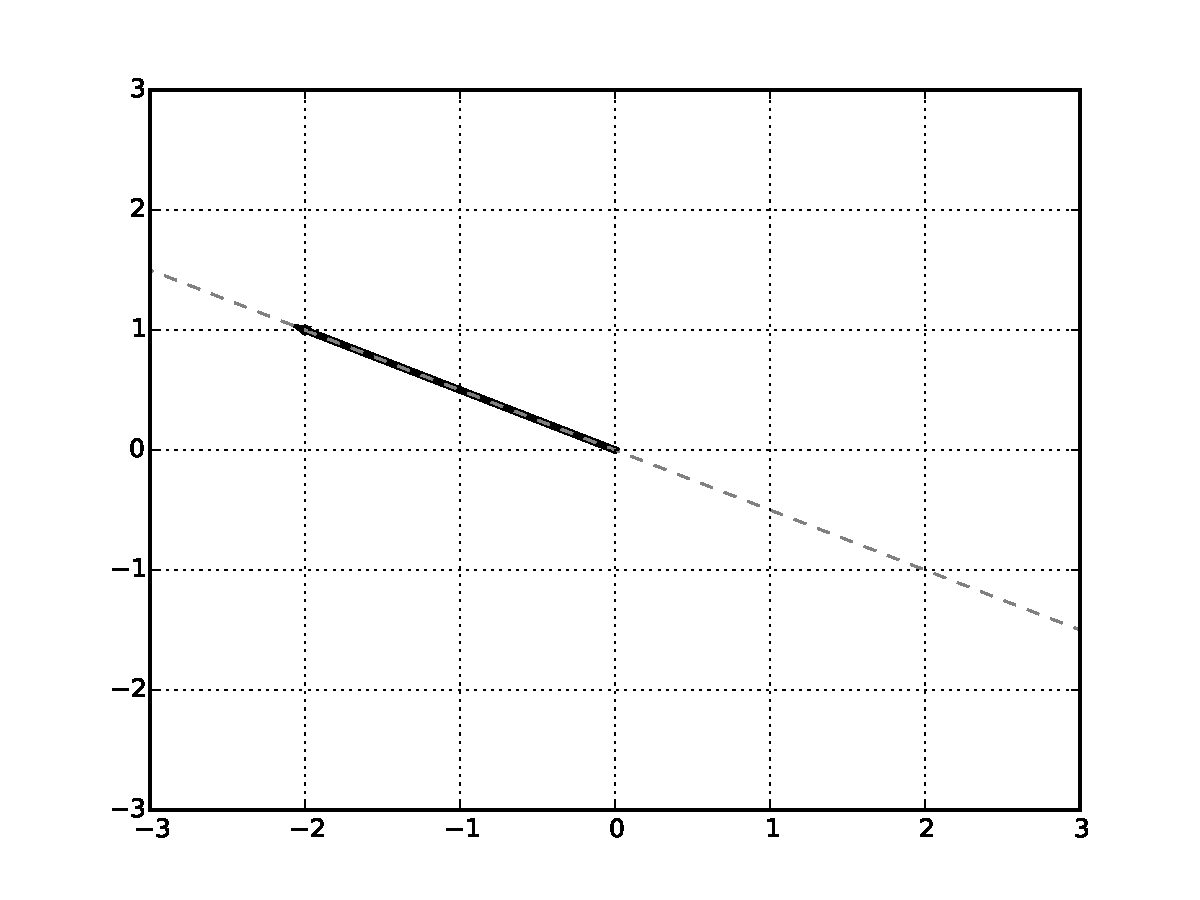
\includegraphics[width=0.7\linewidth]{figs/ex3_6_1b.pdf}

\begin{verbatim}
A= Matrix(2, 2, [1, 2, 2, 4])

sols= solve(Eq(A*v, zeros(A.rows, 1)))[0]
## Or simply
nsp= A.nullspace()[0]

plt.plot((0, nsp[0]*3), (0, nsp[1]*3))

plt.plot((-nsp[0]*3, nsp[0]*3), (-nsp[1]*3, nsp[1]*3), color= 'grey',
    linestyle= '--')
plt.arrow(0, 0, float(nsp[0]), float(nsp[1]), 'g', lw= 3)
plt.xlim(-3, 3)
plt.ylim(-3, 3)
plt.grid()
plt.savefig('figs/ex3_6_1b.pdf')
\end{verbatim}

For $\left[\begin{matrix}1 & 0\\1 & 2\\6 & 10\end{matrix}\right]$ we need to solve
$\left[\begin{matrix}x\\x + 2 y\\6 x + 10 y\end{matrix}\right] = \left[\begin{matrix}0\\0\\0\end{matrix}\right]$.
This is for $\left \{ x : 0, \quad y : 0\right \}$.

\begin{verbatim}
A= Matrix(3, 2, [1, 0, 1, 2, 6, 10])

sols= solve(Eq(A*v, zeros(A.rows, 1)))[0]
## Or
A.nullspace() # -> []
\end{verbatim}


For $\left[\begin{matrix}1 & 2\\3 & 4\\5 & 6\end{matrix}\right]$ we have
$\left[\begin{matrix}x + 2 y\\3 x + 4 y\\5 x + 6 y\end{matrix}\right] = \left[\begin{matrix}0\\0\\0\end{matrix}\right]$
solved only for $x= 0; y= 0$

\begin{verbatim}
A= Matrix(3, 2, [1, 2, 3, 4, 5, 6])
sols= solve(Eq(A*v, zeros(A.rows, 1)))[0]
\end{verbatim}

\subsubsection{Exercise 3.6.3}
%-----------------------------
Determine nullspace and nullity for
$\mathbf{A} = \left[\begin{matrix}1 & -2 & -3\\4 & -5 & -6\\7 & -8 & -9\end{matrix}\right]$.

The solution to 
$\left[\begin{matrix}x - 2 y - 3 z\\4 x - 5 y - 6 z\\7 x - 8 y - 9 z\end{matrix}\right] =
\left[\begin{matrix}0\\0\\0\end{matrix}\right]$.

is $\left \{ x : - z, \quad y : - 2 z\right \}$. Rearranged in vector form we have
$\left[\begin{matrix}x\\y\\z\end{matrix}\right] =
\left[\begin{matrix}-z\\-2z\\z\end{matrix}\right] =
z(\left[\begin{matrix}-1\\-2\\1\end{matrix}\right])
$ for $z$ being any real. Note therefore that the nullspace is the solution to the
linear system.

The nullity is the dimension of the nullspace. In this case only one vector makes
the nullspace, hence $nullity(\mathbf{A}) = 1$

\begin{verbatim}
A= Matrix([[1, -2, -3],
           [4, -5, -6],
           [7, -8, -9]])
x,y,z= symbols('x,y,z')
v= Matrix([x, y, z])
sols= solve(Eq(A*v, zeros(A.rows, 1)), x)[0]
v.subs(sols)
# Also
nsp= A.nullspace() # -> [[-1, -2, 1]]
nlty= len(nsp)     # -> 1
\end{verbatim}

For $\mathbf{A} = \left[\begin{matrix}2 & -2 & -2\\4 & -4 & -4\\8 & -8 & -8\end{matrix}\right]$
the linear systen to solve is
$\left[\begin{matrix}2 x - 2 y - 2 z\\4 x - 4 y - 4 z\\8 x - 8 y - 8 z\end{matrix}\right] =
\left[\begin{matrix}0\\0\\0\end{matrix}\right]$. Solved for $\left \{ x : y + z\right \}$.
Substituing the results in \textbf{v} we have the nullspace:

$
\mathbf{v_{sol}} = \left[\begin{matrix}x\\y\\z\end{matrix}\right] =
\left[\begin{matrix}y + z\\y\\z\end{matrix}\right] =
y(\left[\begin{matrix}1\\1\\0\end{matrix}\right]) + z(\left[\begin{matrix}1\\0\\1\end{matrix}\right])
$

The nullspace is made of two vectors $y(\left[\begin{matrix}1\\1\\0\end{matrix}\right]) + z(\left[\begin{matrix}1\\0\\1\end{matrix}\right])$
hence the nullity is 2. Note that $rank(\mathbf{A}) = 1$ consistent with $nullity(\mathbf{A}) + rank(\mathbf{A}) = n$

\begin{verbatim}
A= Matrix([[2, -2, -2],
           [4, -4, -4],
           [8, -8, -8]])
sols= solve(Eq(A*v, zeros(A.rows, 1)), x)
v.subs(sols)
# Equivalent to
y*Matrix([1,1,0]) + z*Matrix([1, 0, 1])
# Same as
nsp= A.nullspace()
nlty= len(nsp)
\end{verbatim}

This system
$\left[\begin{matrix}2 x + 9 y - 3 z\\5 x + 6 y - z\\9 x + 8 y - 9 z\end{matrix}\right] =
\left[\begin{matrix}0\\0\\0\end{matrix}\right]$
has solution only for $\left [ \left \{ x : 0, \quad y : 0, \quad z : 0\right \}\right ]$
hence the nullspace is the zero vector and the nullity is 0. In fact, the
dimension of the zero vector is zero.

\begin{verbatim}
A= Matrix([[2, 9, -3],
           [5, 6, -1],
           [9, 8, -9]])
sols= solve(Eq(A*v, zeros(A.rows, 1)))
nsp= A.nullspace() # -> []
nlty= len(nsp)     # -> 0
\end{verbatim}

Same as above for $\mathbf{A}= \left[\begin{matrix}-3 & 1 & -1\\2 & 5 & -7\\4 & 8 & -4\end{matrix}\right]$

\begin{verbatim}
A= Matrix([[-3, 1, -1],
           [2, 5, -7],
           [4, 8, -4]])
sols= solve(Eq(A*v, zeros(A.rows, 1)))
\end{verbatim}

\subsubsection{Exercise 3.6.4}
%-----------------------------

Determine the nullspace and nullity of
$\left[\begin{matrix}1 & 2 & 3 & 4 & 5 & 6 & 7\\
                     8 & 9 & 10 & 11 & 12 & 13 & 14\\
                     15 & 16 & 17 & 18 & 19 & 20 & 21\\
                     22 & 23 & 24 & 25 & 26 & 27 & 28\\
                     29 & 30 & 31 & 32 & 33 & 34 & 35\end{matrix}\right]$

Nullspace is
$
\left [ \left[\begin{matrix}1\\-2\\1\\0\\0\\0\\0\end{matrix}\right], \quad
        \left[\begin{matrix}2\\-3\\0\\1\\0\\0\\0\end{matrix}\right], \quad
        \left[\begin{matrix}3\\-4\\0\\0\\1\\0\\0\end{matrix}\right], \quad
        \left[\begin{matrix}4\\-5\\0\\0\\0\\1\\0\end{matrix}\right], \quad
        \left[\begin{matrix}5\\-6\\0\\0\\0\\0\\1\end{matrix}\right]\right ]
$ contaning five vectors, five is the nullity of \textbf{A}.

\begin{verbatim}
x1,x2,x3,x4,x5,x6,x7= symbols('x1:8')
A= Matrix(5, 7, range(1, 36))
sols= solve(Eq(A*v, zeros(A.rows, 1)))
v.subs(sols) # Nullspace. You could read out the nullspace vectors from here
nsp= A.nullspace()
nly= len(A) # 5
\end{verbatim}

\subsubsection{Exercise 3.6.5}
%-----------------------------

Determine bases for row, column and null space for
$\mathbf{A} = \left[\begin{matrix}1 & -4 & -9\\2 & 5 & -7\end{matrix}\right]$.

In other words, we need to find a set of \textbf{linearly independent} vectors such that
every vector in the given vector space (e.g. row space) is \textbf{linearly dependent} of these
vectors. Bases or coordinates are the basic building blocks to represent a vector
space.

To find a basis for the rows of a matrix (i.e. for this vector space) we need to
put the matrix un RREF. The rows of the RREF matrix are linearly independent. For
the rows in \textbf{A},
$\mathbf{A_{rref}} =
\left[\begin{matrix}1 & 0 & - \frac{73}{13}\\0 & 1 & \frac{11}{13}\end{matrix}\right] =
\left[\begin{matrix}13 & 0 & -73\\0 & 13 & 11\end{matrix}\right]$,

the rows of $\mathbf{A_{rref}}$ are the bases for the row space of $\mathbf{A}$.

The basis for the column vector can be obtained by looking at the leading 1s in
$A_{rref}$, these are $\left[\begin{matrix}1 & 0\\0 & 1\end{matrix}\right]$. \emph{
The same conclusion is reached by transposing \textbf{A} and repeating the reasoning
for the row space. Like \texttt{A.transpose().rref()}}

The basis for the nullspace is given by a nullspace itself \texttt{A.nullspace()}
which is $\left[\begin{matrix}\frac{73}{13}\\- \frac{11}{13}\\1\end{matrix}\right]$.
In this case the nullity is 1.

\begin{verbatim}
A= Matrix(2, 3, [1, -4, -9, 2, 5, -7])
B= Matrix(3, 2, [1, 3, 2, 5, -14, -37])
C= Matrix([[1, 3, -9, 5],
           [2, 6, 7, 1],
           [1, 3, -8, 1]])
rbasis= rref= A.rref()
cbasis= rref.A.transpose().rref()
nspbasis= A.nullspace()
\end{verbatim}

\subsubsection{Exercise 3.6.7}
%-----------------------------

Determine whether the following system have \emph{infinite}, \emph{unique}, or
\emph{no} solutions.

Without actually solving the system we can get the type of solution by looking
at the rank of coefficient matrix and augmented matrix:

\begin{itemize}
\item \textbf{Infinite solutions} $rank(\mathbf{A}) = rank(\mathbf{A_{augmented}}) < nrow(\mathbf{A})$
\item \textbf{Unique solution} $rank(\mathbf{A}) = rank(\mathbf{A_{augmented}}) = nrow(\mathbf{A})$
\item \textbf{No solution} $rank(\mathbf{A}) \neq rank(\mathbf{A_{augmented}})$
\end{itemize}


\begin{verbatim}
def numSolutions(A, b):
    rankA= A.rank()
    rankA_aug= Matrix(numpy.hstack([A, b])).rank()
    n= A.rows
    print 'nrow(A)= %s' %(n)
    print 'rank(A)= %s' %(rankA)
    print 'rank(A_aug)= %s' %(rankA_aug)
    if rankA == rankA_aug == n:
        return 'unique solution'
    elif rankA == rankA_aug < n:
        return 'oo solutions'
    elif rankA != rankA_aug:
        return 'no solutions'
    else:
        return None

A= Matrix([[1,2,3],
           [4,5,6],
           [7,8,9]])
b= Matrix([1,2,4])
numSolutions(A, b) # No solutions
\end{verbatim}

Consider the system

$$
A = \left[\begin{matrix}2x +& 5y & -3z & -7w\\
                        1x +& 1y & -4z & -8w\\
                        3x +& 4y & + 0z  & +1w \\
                        5x +& 21y & -1z & +3w
        \end{matrix}\right]
b= \left[\begin{matrix}0\\9\\6\\2\end{matrix}\right]
$$

It has a unique solution has showed here using ranks and verified by actually solving the
system. Solution are

$$
\left[\begin{matrix}x\\y\\z\\w\end{matrix}\right] =
\left[\begin{matrix}\frac{332}{117}\\
                    - \frac{545}{351}\\
                    - \frac{1091}{117}\\
                      \frac{1298}{351}
    \end{matrix}\right]
$$

\begin{verbatim}
A= Matrix([[2, 5, -3, -7],
           [1, 1, -4, -8],
           [3, 4, 0, 1],
           [5, 21, -1, 3]])
b= Matrix([0, 9, 6, 2])
numSolutions(A, b) ## Unique solution
nrow(A)= 4
rank(A)= 4
rank(A_aug)= 4

## Solve
xyzw_sols= A.solve(b)
\end{verbatim}

If we add a redundant row, the system is overdetermined and has infinite solutions:

$$
\mathbf{A}= \left[\begin{matrix}2 & 5 & -3 & -7\\1 & 1 & -4 & -8\\3 & 4 & 0 & 1\\5 & 21 & -1 & 3\\5 & 21 & -1 & 3\end{matrix}\right]
\mathbf{b}= \left[\begin{matrix}0\\9\\6\\2\\2\end{matrix}\right]
$$

Note also the exception thrown by \texttt{Matrix.solve} \textcolor{blue}{\texttt{
ValueError: For over-determined system, M, having more rows than columns,
try M.solve\_least\_squares(rhs).}}. Using least squares we get the
unique solution.

\begin{verbatim}
A= Matrix([[2, 5, -3, -7],
           [1, 1, -4, -8],
           [3, 4, 0, 1],
           [5, 21, -1, 3],
           [5, 21, -1, 3]])
b= Matrix([0, 9, 6, 2, 2])
numSolutions(A, b) ## 'oo solutions'
nrow(A)= 5
rank(A)= 4
rank(A_aug)= 4

A.solve(b) ## ValueError: For over-determined system

## Use linear least squares:
def linlsq(A, b):
    betas= (A.transpose() * A).inv() * A.transpose() * b
    return betas

## Same as sympy function:
linlsq(A, b)             ## [332/117], [-545/351], [-1091/117], [1298/351]
A.solve_least_squares(b) ## 
\end{verbatim}

\subsubsection{Exercise 3.6.8a}
%------------------------------

Test if the vectors \textbf{u} are in \emph{nullspace} of the corresponding
matrices:

\begin{itemize}
\item Get the nullspace of \textbf{A} by solving $\mathbf{Av= O}$
\item Test if \textbf{u} is a linear combination of the nullspace
\end{itemize}

To find the nullspace either use \sympy \texttt{Matrix.nullspace()} or solve the
system $\mathbf{Av= O}$ where \textbf{v} is a general vector of unknowns $[x_1\ x_2\ ...\ x_n]$.
Then, to extract the nullspace from the solution(s), substitute the solutions in
\textbf{v} and extract the coeffcients. For matrix

$$
\mathbf{A}= \left[\begin{matrix}1 & 1 & -1\\2 & -1 & 0\\5 & 2 & -3\end{matrix}\right]
$$

solve:

$$
\left[\begin{matrix}x_{1} + x_{2} - x_{3}\\2 x_{1} - x_{2}\\5 x_{1} + 2 x_{2} - 3 x_{3}\end{matrix}\right] = \left[\begin{matrix}0\\0\\0\end{matrix}\right]
$$

The solution are substituted in \textbf{v} and the coefficients extracted:

$$
sols= \left \{ x_{1} : \frac{x_{3}}{3}, \quad x_{2} : \frac{2 x_{3}}{3}\right \} =
\left[\begin{matrix}\frac{x_{3}}{3}\\\frac{2 x_{3}}{3}\\x_{3}\end{matrix}\right] =
x_3(\left[\begin{matrix}\frac{1}{3}\\\frac{2}{3}\\1\end{matrix}\right])
$$

So the nullspace is $x(\left[\begin{matrix}\frac{1}{3}\\\frac{2}{3}\\1\end{matrix}\right])$
for any real $x$.

\begin{verbatim}
u= Matrix([1, 2, 3])
A= Matrix([[1,1,-1], [2, -1, 0], [5, 2, -3]])

## Nullspace
x1,x2,x3= symbols('x1:4')
v= Matrix([x1, x2, x3])
sols= solve(Eq(A*v, zeros(A.rows, 1)))[0]
nsp= v.subs(sols) / x3

## Or simply
nsp= A.nullspace()
\end{verbatim}

Now, is the vector \textbf{u} part of the nullspace? See
\href{http://mathworld.wolfram.com/LinearlyDependentVectors.html}{LinearlyDependentVectors}
on Wolfram for different ways to test linear dependence between vectors.

\begin{verbatim}
## Test for linear dependence between u and nullspace vector:
detm= Matrix(2,2, [nsp.dot(nsp), nsp.dot(u),
             u.dot(nsp),   u.dot(u)]).det() ## == 0 -> u is in the nullspace

## Or test if 2xn matrix has rank < 2
Matrix(numpy.hstack([nsp, u])).transpose().rank() < 2 # rank<2. Vectors are lin.
                                                      # dep.
\end{verbatim}

Actually, the simple way is just to test:

$$
\mathbf{Au = O} =
\left[\begin{matrix}1 & 1 & -1\\2 & -1 & 0\\5 & 2 & -3\end{matrix}\right]
\left[\begin{matrix}1\\2\\3\end{matrix}\right] =
\left[\begin{matrix}0\\0\\0\end{matrix}\right]
$$

Since the nullspace is the set of vectors that transformed by \textbf{A} results
in the zero vector.

\begin{verbatim}
Eq(A*u, zeros(A.rows, 1)) ## True; u is in the nullspace of A
\end{verbatim}

\subsubsection{Exercise 3.6.8b}
%------------------------------

\begin{verbatim}
u= ones(3, 1)
B= Matrix(2, 3, [1, 4, -5,
                -7, 5,  2])
Eq(B*u, zeros(B.rows, 1)) # True: u is in the nullspace

## Or: extract nullspace from B and check if u is linearly dependent
nsp= B.nullspace()[0]
Matrix(numpy.hstack([nsp, u])).rank() < 2 # true: nullspace and u are lin dep
\end{verbatim}

\subsubsection{Exercise 3.6.8c}
%------------------------------

In case $\mathbf{u} = \left[\begin{matrix}1\\1\\1\end{matrix}\right];
\mathbf{C}= \left[\begin{matrix}1 & 3 & -9 & 5\\2 & 6 & 7 & 1\\1 & 3 & -8 & 1\end{matrix}\right]
$ dimensions are incompatible. Trying to compute \texttt{C*u} gives
\textcolor{blue}{\texttt{ShapeError: Matrices size mismatch.}} Consequently \textbf{u}
cannot be in the nullspace of \textbf{C}.

\begin{verbatim}
u= Matrix([2,1,5])
C= Matrix(2, 4, [1, 2, 3, 4,
                 5, 6, 7, 8])

Eq(C*u, zeros(C.rows, 1)) # ShapeError: Matrices size mismatch.
\end{verbatim}

\subsubsection{Exercise 3.6.8d}
%------------------------------

For $\mathbf{u}= \left[\begin{matrix}1\\3\\-4\\7\end{matrix}\right];
\mathbf{D}= \left[\begin{matrix}1 & -2 & 6 & 1\\3 & -6 & 7 & 8\\5 & 2 & 1 & 7\\1 & 6 & 3 & 2\end{matrix}\right];
\mathbf{Du} \neq \mathbf{O}$ \emph{I.e.} \textbf{u} is not in the nullspace. Note also
that $rank(\mathbf{D}) = nrow(\mathbf{D})$ and, consequently, $nullspace(\mathbf{D}) = null$.
Hence no vector is in the nullspace of \textbf{D}.


\begin{verbatim}
u= Matrix([1, 3, -4, 7])
D= Matrix([[1, -2, 6, 1],
           [3, -6, 7, 8],
           [5, 2, 1, 7],
           [1, 6, 3, 2]])

Eq(D*u, zeros(D.rows, 1)) # False, u not in nullspace

# Not also:
nsp= D.nullspace() # empty []
D.rank() == D.rows # Matrix is full rank
\end{verbatim}
\section{5. Linear Transformations}
% *********************************

\subsection{Introduction to linear transformations}
% =================================================

A \emph{transformation} or \emph{mapping} converts \underline{every} element in
the starting set (\textbf{domain}) to a \underline{unique} element in the arrival
sets (\textbf{codomain}). A transformation $T$ between spaces $V$ and $W$ is linear 
if and only if

\textbf{A)} $T(\mathbf{u} + \mathbf{v}) = T(\mathbf{u}) + T(\mathbf{v})$ and

\textbf{B)} $T(k\mathbf{u}) = kT(\mathbf{u})$

\subsubsection{Exercise 5.1.1}
%-----------------------------

Consider the transformation $T(\mathbf{u}) = \mathbf{Au}$. Determine $T(\mathbf{u})$
for the given \textbf{u}.

\begin{verbatim}
A= Matrix([[0, 1], [1, 0]])
u_a= Matrix([1, 3])
u_b= Matrix([-1, 5])
u_c= Matrix([sqrt(2), 1])
u_d= Matrix([-2, -3])

plt.rc('font', size= 8)
fig, ax= plt.subplots(1, 4)
for i, u in enumerate([u_a, u_b, u_c, u_d]):
    Tu= A.dot(u)
    ax[i].plot( (0, u[0]), (0, u[1]), color= 'blue', label= 'u' )
    ax[i].plot( (0, Tu[0]), (0, Tu[1]), color= 'red', label= 'T(u)' )
    ax[i].grid()

ax[0].legend(frameon= False)    
fig.set_size_inches(10, 2)
plt.savefig('figs/ex5_1_1a.pdf', bbox_inches='tight')
\end{verbatim}

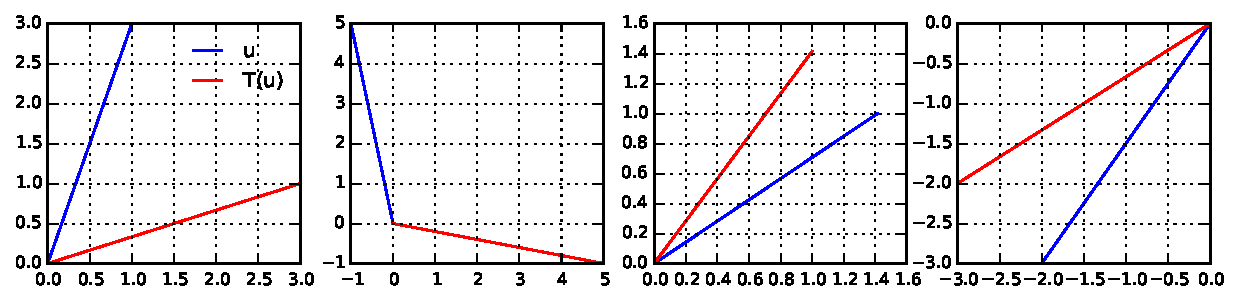
\includegraphics[width=1.2\linewidth]{figs/ex5_1_1a.pdf}

\subsubsection{Exercise 5.1.5}
%-----------------------------

Given the transformation (mapping) \ref{eq:ex5_1_5} in $\mathbb{R}^3$:

\begin{equation}\label{eq:ex5_1_5}
T{\left (\left[\begin{matrix}x\\y\\z\end{matrix}\right] \right )} =
\left[\begin{matrix}x + y\\
                    y + z\\
                    z + x\end{matrix}\right]
\end{equation}

determine whether the transformation \ref{eq:ex5_1_5} is linear.

In other words, we need to check whether the conditions \textbf{A} and
\textbf{B} above are satisfied.

First define a function with the transformation $T$ to be tested. Then define two generic
vectors \textbf{u} and \textbf{v} and see if applying $T$ satisfies the conditions
for linearity.

\begin{verbatim}
x, y, z, s, t, l, k= symbols('x y z s t l k', real= True)

def T(u):
    Tu= Matrix([u[0] + u[1],
                u[1] + u[2],
                u[2] + u[0]])
    return(Tu)
\end{verbatim}

Get two vectors and test conditions for linearity:

\begin{verbatim}
u= Matrix([x, y, z])
v= Matrix([s, t, l])

## Cond A:
assert (T(u + v)) - (T(u) + T(v)) == zeros(3, 1)

## Cond B:
assert (T(k * u) - k * T(u)).expand() == zeros(3, 1)
\end{verbatim}

Assertions return \texttt{True} hence the transformation \texttt{T} is linear.

Pay attention how the conditions for equality are tested in \sympy. We subtract
one term from the other and check the result is zero, in this case the zero vector
in $\mathbb{R}^3$ $[0\ 0\ 0]^T$. Using the double equal sign \texttt{==} would return
\texttt{False} in the second assertion since \texttt{==} tests for identity of form
not for \textbf{symbolic identity}. See also \href{https://github.com/sympy/sympy/wiki/Faq}{
Why does SymPy say that two equal expressions are unequal?}

The trasformation $T$:

$$
T(\left[\begin{matrix}x\\y\\z\end{matrix}\right]) = \left[\begin{matrix}\sqrt{x}\\\sqrt{y}\\\sqrt{z}\end{matrix}\right]
$$

Is not linear since $\sqrt{a + b} = \sqrt{a} + \sqrt{b}$ is not satisfied.

\begin{verbatim}
def T(u):
    Tu= Matrix([sqrt(u[0]), sqrt(u[1]), sqrt(u[2])])
    return(Tu)
    
u= Matrix([x, y, z])
v= Matrix([s, t, l])

## Cond A
(T(u + v)).expand() - (T(u) + T(v)).expand() == zeros(3, 1) ## False

## Cond B
(T(k * u)).expand() - (k * T(u)).expand() == zeros(3, 1) ## False
\end{verbatim}

\subsubsection{Exercise 5.1.6 a}
%-------------------------------

This is an helper function which might be useful elsewhere \footnote{See also
on StackOverflow \href{http://stackoverflow.com/questions/29434911/sympy-how-to-get-zero-for-absent-constant-term/}
{How to get zero for absent constant term.}}. Here we use it to implement the
tranformation \ref{eq:ex5_1_6a} where we need to swap the coefficients of a
polynomial. By returning a dictionary of terms and coefficients, \texttt{getCoeffDict}
makes the manipulation of coefficients easier.

\begin{equation}\label{eq:ex5_1_6a}
T(c_2 x^2 + c_1 x + c_0) = c_0 x^2 + c_1 x + c_2
\end{equation}

\begin{verbatim}
def getCoeffDict(exprs, x):
    """Return a dict of coefficients for each power of the variable `x` in
    expression `exprs`. Examples:
    
        >>> x, a, b, c= symbols('x a b c')
        >>> getCoeffDict(a*x**2 + b*x + c, x)
        {x**2: a, x: b, 1: c}
        >>> getCoeffDict(a*x**2, x)
        {1: 0, x: 0, x**2: a}
    """
    exprs= exprs.expand()
    n= Poly(exprs).degree(x)
    cdict= {}
    for i in range(0, n+1):
        cdict[x**i]= exprs.coeff(x, i)
    return(cdict)
\end{verbatim}

Let's proceede testing whether \ref{eq:ex5_1_6a} is a linear tranformation. Note
that the transformation \ref{eq:ex5_1_6a} works in polynomial space, not in
Euclidean space. However, the approach remains the same.

\begin{enumerate}
\item{Define the transformation of interest}
\begin{verbatim}
def T(p):
    k= getCoeffDict(p, x)
    Tp= k[1]*x**2 + k[x]*x + k[x**2]
    return(Tp)
\end{verbatim}

\item{Get two generic vectors:}
\begin{verbatim}
k= symbols('k', nonzero= True)
c0, c1, c2= symbols('c0 c1 c2')
b0, b1, b2= symbols('b0 b1 b2')

p= c2*x**2 + c1*x + c0
q= b2*x**2 + b1*x + b0
\end{verbatim}

\item Test condition $T(\mathbf{u + v}) = T(\mathbf{u}) + T(\mathbf{v})$
\begin{verbatim}
( (T(p+q)) - (T(p)+T(q)) ).expand() == 0 ## True
\end{verbatim}

\item Test condition $T(k\mathbf{u}) = kT(\mathbf{u})$
\begin{verbatim}
(T(k * p)) - (k * T(p)).expand() == 0 ## True
\end{verbatim}
\end{enumerate}

\subsubsection{Exercise 5.1.6 b}
%-------------------------------

Similar to \textit{a} above. For

$$
T(c_2 x^2 + c_1 x + c_0) = c_2^2 x^2 + c_1^2 x + c_0^2
$$

\begin{verbatim}
def T(p):
    k= getCoeffDict(p, x)
    Tp= k[x**2]**2 * x**2 + k[x]**2 * x + k[1]**2
    return(Tp)

p= c2*x**2 + c1*x + c0
q= b2*x**2 + b1*x + b0

# Is `kT(u) = T(ku)`?
((k*T(p)).expand() - (T(k*p)).expand()) == 0 # False
\end{verbatim}

Condition $T(k\mathbf{u}) = kT(\mathbf{u})$ can't be satisfied hence the
transformation is not linear.

$$
k \left(c_{0}^{2} + c_{1}^{2} x + c_{2}^{2} x^{2}\right) \neq c_{0}^{2} k^{2} + c_{1}^{2} k^{2} x + c_{2}^{2} k^{2} x^{2}
$$

\subsubsection{Exercise 5.1.7 a}
%-------------------------------

Check whether matrix transposition is a linear transformation. See \texttt{?Matrix.equals}
for testing matrix equality.

\begin{verbatim}
def T(A):
    return A.transpose()

a, b, c, d, e, f, g, h, i= symbols('a:i')
A= Matrix(2,2, [a,b,c,d])
B= Matrix(2,2, [f,g,h,i])

T(A+B).equals(T(A) + T(B)) ## True
(k*T(A)).equals(T(k*A))    ## True
\end{verbatim}

Matrix transposition \emph{is} linear.

Again, we are not working in Euclidean space but the approach is the same. This
is \emph{matrix space of size \emph{n} by \emph{n}}.

\subsubsection{Exercise 5.1.9}
%-------------------------------

Test whether \emph{integration} is linear. Note that integration maps from space
$C{0, 1}$ to $\mathbb{R}$.

\begin{verbatim}
f= Function('f')(x)
def T(f):
    return integrate(f, (x, 0, 1))
    
x= symbols('x', real= True, nonnegative= True, nonzero= False)
f= Function('f')(x)
g= Function('g')(x)

(T(f+g)).equals(T(f) + T(g)) ## Returns None
(k*T(f)).equals(T(k*f))  ## True
\end{verbatim}

First condition is satisified since:

$$
\int_{0}^{1} f{\left (x \right )} + g{\left (x \right )}\, dx = \int_{0}^{1} f{\left (x \right )}\, dx + \int_{0}^{1} g{\left (x \right )}\, dx
$$

\sympy returns \texttt{None} and this might be ok since \emph{$[$\texttt{Function.equals} returns$]$ None
(instead of T/F) for an expression that *is* zero but won't simplify to zero.}
(See \href{https://groups.google.com/forum/#!topic/sympy/xP_uM49pXeo}{\sympy discussion group})

\subsection{5.2 Kernel and range of a linear transformation}
% ==========================================================

The \textbf{kernel} of a linear transformation is the set of domain (starting)
values which map to zero in the codomain (arrival). \emph{I.e.} the kernel of
$T$ is:

$$
T(\mathbf{v}) = \mathbf{O})
$$

The \textbf{range} or \textbf{image} of a linear transformation is the
subset of values in the codomain $W$ where a linear transformation $T$ can arrive.
Formally:

$$
range(T) = {T(\mathbf{v}) | \mathbf{v} in V}
$$
\section{6. Determinant and the Inverse Matrix}
% *********************************************

Remember that division is not a valid operation in matrix algebra, \emph{e.g.}
$1/\mathbf{A}$ or $\mathbf{A/B}$ are not meanigful. Instead of \emph{dividing by} a matrix
we \emph{multiply by the inverse} of that matrix. For example, to find the vector of \textbf{x}
in $\mathbf{Ax = b}$ we can't do $\mathbf{x= b/A}$ but we can do
$\mathbf{A^{-1}Ax = A^{-1}b; \quad x = A^{-1}b}$. That's why matrix inversion is
so important.

To compute the inverse matrix we need to pass by its determinant.
In particular we need to compute $1/det(\mathbf{A})$. This means that if
$det(\mathbf{A}) = 0$ matrix inversion is not possible and the matrix is said
to be \emph{singular}. Therefore, the determinant
can tell whether a linear system as a unique solution. I.e. if $det(\mathbf{A}) \neq 0$
then you have a unique solution. This is why determinants are important.

Calculating the determinant is a lengthy process that increases very quickly with
the size of the matrix, like $O(n!)$ or $O(n^3)$ with $n$ the size of the matrix
\footnote{http://en.wikipedia.org/wiki/Computational\_complexity\_of\_mathematical\_operations\#Matrix\_algebra}.
This means that shortcuts had to be invented to make the process feasible for large
matrices, for example by splitting the original matrix in smaller and easier
matrices. The various matrix decompositions also known as factorizations, like LU decomposition
are aimed at reducing such complexity.

\subsection{Determinant of a Matrix}
% ==================================

The \textbf{determinant} of a \emph{square} matrix is a unique value the tells
whether the matrix is invertible. In turn this tells whether the system $\mathbf{Ax = b}$
has a unique solution.

\subsubsection{Exercise 6.1.4}
%-----------------------------

\emph{Geometric interpretation of the $det(\mathbf{A})$} The determinant of a 2x2 matrix
is the area of the parallelogram defined by the coordinates of the column vectors.

For $\mathbf{A} = \left[\begin{matrix}2 & 1\\0 & 3\end{matrix}\right]$ show that
$det(\mathbf{A}) = 6$ is the area of the parallelogram defined by the points (\underline{column
vectors})  $\left[\begin{matrix}2 & 0\end{matrix}\right]^T$ and
$\left[\begin{matrix}1 & 3\end{matrix}\right]^T$

Note that the vertices in varibale \texttt{vert} are $
\left[\begin{matrix}0\\0\end{matrix}\right], \quad
\left[\begin{matrix}2\\0\end{matrix}\right], \quad
\left[\begin{matrix}3\\3\end{matrix}\right], \quad
\left[\begin{matrix}1\\3\end{matrix}\right]
$ where the coordinates $(3,3)$ are the row sums.

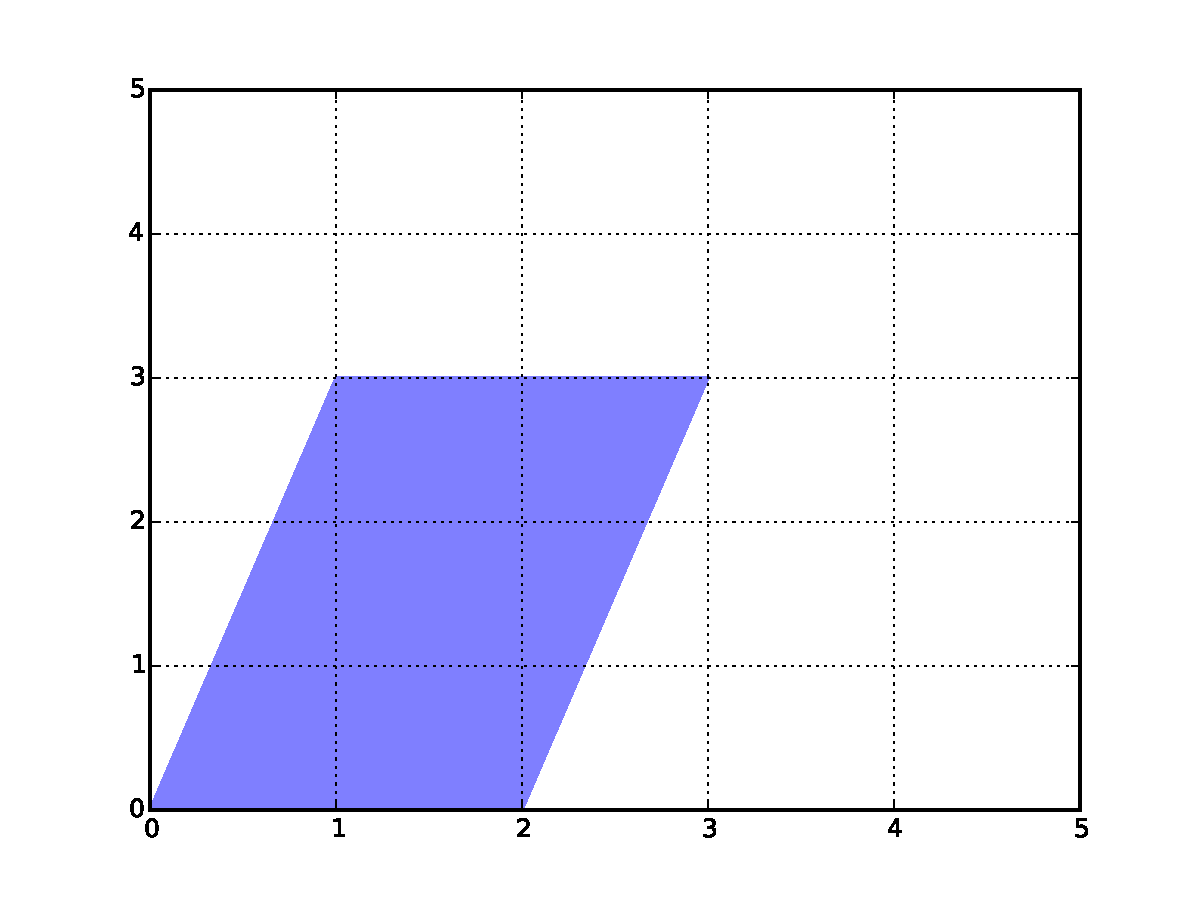
\includegraphics[width=\linewidth]{figs/ex6_1_4.pdf}

\begin{verbatim}
from matplotlib import patches

A= Matrix(2, 2, [2, 1, 0, 3])
A.det() # 6

verts= [(0, 0),
        A.col(0),
        (sum(A.row(0)), sum(A.row(1))),
        A.col(1)]

parall= patches.Polygon(verts, color= 'b', alpha= 0.5)
fig = plt.figure()
ax = fig.add_subplot(1, 1, 1)
ax.add_patch(parall)
ax.set_xlim((0, 5))
ax.set_ylim((0, 5))
plt.grid()
plt.draw()
fig.savefig('figs/ex6_1_4.pdf')
plt.close()
\end{verbatim}

Note that a negative determinant means that area is rotated.

\begin{verbatim}
A1= Matrix(2,2, [1, 2, 3, 0])
A1.det() # -6
\end{verbatim}

Similarly, the determinant of a 3x3 matrix is the volume of the parallelepid described
by the matrix coordinates.

\subsubsection{Exercise 6.1.5}
%-----------------------------

Determine whether the following system has a unique solution

$$
\left [
2 x + 3 y = -2, \quad
5 x - 2 y = 14
\right ]
$$

The system can be re-written in matrix form as

$$
\mathbf{Ax= b} \quad
\left[\begin{matrix}
2 x + 3 y\\5 x - 2 y
\end{matrix}\right] = \left[\begin{matrix}-2\\14\end{matrix}\right]
$$

The determinant of \textbf{A} is $det(\mathbf{A})= -19 \neq 0$, so the system has
a unique solution for $x= 2, y= -2$

\begin{verbatim}
eq1= Eq(2*x + 3*y, -2)
eq2= Eq(5*x - 2*y, 14)
sols= solve([eq1, eq2])

# Can be re-written as 
A= Matrix(2, 2, [2, +3, 5, -2])
det(A) != 0 # True -> Unique solution
b= Matrix([-2, 14])
X= Matrix([x, y])
axb= Eq(A*X, b)
solve(axb) # Same as above
\end{verbatim}

Note that a unique solution is found for any values of the vector \textbf{b}, the
right hand side of the equations or responses. What decides whether the system has
a unique solution are the coefficients in the matrix \textbf{A}, \emph{i.e.} the
left hand side of the equation or predictors. For example:

\begin{verbatim}
X= Matrix([x, y])
A= Matrix(2, 2, [2, +3, 5, -2])
b1= Matrix([-2, 14])
b2= Matrix([7, 5])
b3= Matrix([pi, pi])

for b in [b1, b2, b3]:
    print solve(Eq(A*X, b))
# {x: 2, y: -2}
# {x: 29/19, y: 25/19}
# {x: 5*pi/19, y: 3*pi/19}
\end{verbatim}

\subsection{Determinant of other matrices}
% ========================================

\subsubsection{Exercise 6.2.2}
%-----------------------------

Show that $det(\left[\begin{matrix}
\mathbf{i} & \mathbf{j} & \mathbf{k} \\
7 & 3 & -2\\
4 & 2 & 7
\end{matrix}\right]) =
25 \mathbf{i} - 57 \mathbf{j} + 2 \mathbf{k}$

\begin{verbatim}
i,j,k= symbols('i j k')
M= Matrix(3, 3, [i, j, k, 7, 3, -2, 4, 2, 7])
M.det() #
\end{verbatim}

\subsubsection{Exercise 6.2.3}
%-----------------------------

find $x$ so that
$$
det(\left[\begin{matrix}1 & 0 & -3\\5 & x & -7\\3 & 9 & x - 1\end{matrix}\right]) = 0
$$

We have $det(\mathbf{M}) = x^{2} + 8 x - 72$ , so to have $x^{2} + 8 x - 72 = 0$
we need $x = -4 + 2 \sqrt{22}, \quad x= - 2 \sqrt{22} - 4$. As shown by substituting
these solutions in \textbf{M} and calculating the determinant.

\begin{verbatim}
M= Matrix([[1, 0, -3],
           [5, x, -7],
           [3, 9, x-1]])

detm= det(M)
eq= Eq(detm, 0)
sols= solve(eq)
det(M.subs(x, sols[0])) == 0 # True
det(M.subs(x, sols[1])) == 0 # True
\end{verbatim}

\subsubsection{Exercise 6.2.4}
%-----------------------------


Find the \textbf{cofactor matrix} \textbf{C} of $
\mathbf{A}= \left[\begin{matrix}1 & 0 & 5\\-2 & 3 & 7\\6 & -1 & 0\end{matrix}\right]
$

Cofactor matrix:

$$
\mathbf{C}= \left[\begin{matrix}7 & 42 & -16\\-5 & -30 & 1\\-15 & -17 & 3\end{matrix}\right]
$$

The cofactor matrix is used to calculate the \textbf{inverse} of matrix.

\begin{verbatim}
A= Matrix([[1, 0, 5],
           [-2, 3, 7],
           [6, -1, 0]])
C= A.cofactorMatrix()
\end{verbatim}

Maybe useful to note:

$$
\mathbf{A} = \left[\begin{matrix}x_{1} & x_{2}\\x_{3} & x_{4}\end{matrix}\right] \quad
\mathbf{C_A}= \left[\begin{matrix}x_{4} & - x_{3}\\- x_{2} & x_{1}\end{matrix}\right]
$$

and

$$
\mathbf{A} =  \left[\begin{matrix}x_{1} & x_{2} & x_{3}\\x_{4} & x_{5} & x_{6}\\x_{7} & x_{8} & x_{9}\end{matrix}\right]
\mathbf{C_A}= \left[\begin{matrix}
x_{5} x_{9} - x_{6} x_{8} & - x_{4} x_{9} + x_{6} x_{7} & x_{4} x_{8} - x_{5} x_{7}\\
- x_{2} x_{9} + x_{3} x_{8} & x_{1} x_{9} - x_{3} x_{7} & - x_{1} x_{8} + x_{2} x_{7}\\
x_{2} x_{6} - x_{3} x_{5} & - x_{1} x_{6} + x_{3} x_{4} & x_{1} x_{5} - x_{2} x_{4}
\end{matrix}\right]
$$

\begin{verbatim}
x1,x2,x3,x4,x5,x6,x7,x8,x9= symbols('x1:10')

A= Matrix(2,2,[x1, x2, x3, x4])
A.cofactorMatrix()

A= Matrix(3,3,[x1,x2x,x3,x4,x5,x6,x7,x8,x9])
A.cofactorMatrix()
\end{verbatim}

\subsubsection{Exercise 6.2.5}
%-----------------------------

The inverse of \textbf{A} is:

$$
\mathbf{A}^{-1} = \frac{1}{det(\mathbf{A})} adj(\mathbf{A})
$$

where the \emph{adjoint} of \textbf{A} is the transpose of the cofactor matrix of \textbf{A}:
$adj(\mathbf{A}) = \mathbf{C}^T$

\begin{verbatim}
def inv(A):
    C= A.cofactorMatrix()
    adj= C.transpose()
    inva= (1 / det(A)) * adj
    return inva
\end{verbatim}

Find the inverse of the following matrices.

\begin{verbatim}
A= Matrix(2, 2, [9, 2, 13, 3])
inv(A) # checked against A.inv()

D= Matrix(3, 3, [3, -5, 3,
                 2, 1, -7,
                 -10, 4, 5])
inv(D)
\end{verbatim}

\subsubsection{Exercise 6.2.12}
%-----------------------------

Find the values of $k$ for which the matrix
$\mathbf{A} = \left[\begin{matrix}k & 1 & 2\\0 & k & 2\\5 & -5 & k\end{matrix}\right]$
is invertible. Since inversion requires $det(\mathbf{A}) \neq 0$, we need to get
the determinant of \textbf{A} and
solve it for $k$. Values of $k$ that are not solutions of $det(\mathbf{A}) = 0$ make
\textbf{A} invertible.

$det(\mathbf{A}) = k^3 + 10$ solved for $k$ in
$\left [ - \sqrt[3]{10}, \quad
\frac{\sqrt[3]{10}}{2} - \frac{\sqrt{3} i}{2} \sqrt[3]{10}, \quad
\frac{\sqrt[3]{10}}{2} + \frac{\sqrt{3} i}{2} \sqrt[3]{10}\right ]$

\begin{verbatim}
A= Matrix(3, 3, [k, 1, 2,
                 0, k, 2,
                 5, -5, k])

sols= solve(Eq(A.det(), 0))

## Check A is not invertible for k in sols:
A.subs(k, sols[0]).inv()  ## ValueError: Matrix det == 0; not invertible.
A.subs(k, sols[1]).inv()  ## ValueError: Matrix det == 0; not invertible.
A.subs(k, sols[2]).inv()  ## ValueError: Matrix det == 0; not invertible.

## Check it is invertible for other values of k
A.subs(k, 0).inv()
A.subs(k, sols[0]+1).inv()
A.subs(k, sols[2]+1).inv()
\end{verbatim}


\subsection{Properties of determinants}
% =====================================

As noted above, calculating the determinant of large matrices can take ages. However,
the determinant of diagonal and triangular matrices are very easy to compute:
Just multiply the entries along the leading diagonal. This means that if a matrix can be
rearranged in one or more triangular matrices, by means of row operations and decomposition,
than the calculation of the determiant is much simpler.

\subsubsection{Exercise 6.3.1}
%-----------------------------

Find the determinant of $\mathbf{A}= \left[\begin{matrix}1 & 0 & 0\\0 & -10 & 0\\0 & 0 & 1\end{matrix}\right]$.

The matrix is diagonal: Multiply the entries along the leading diagonal
$det(\mathbf{A}) = (1) (-10) (1)= -10$

\begin{verbatim}
def diagprod(A):
    dp= 1
    for i in range(A.rows):
        dp= dp*A[i, i]
    return dp
    
A= Matrix(3, 3, [1, 0, 0,
                 0, -10, 0,
                 0, 0, 1])
diagprod(A) # -10
# Cheack against
diagprod(A) - A.det() == 0 # True
\end{verbatim}

For $\mathbf{B}= \left[\begin{matrix}1 & 0 & 0\\0 & 0 & 1\\0 & 1 & 0\end{matrix}\right]$

The matrix is not diagonal or triangular as such but it can be made diagonal by
swapping rows.

\begin{verbatim}
B= Matrix(3, 3, [1, 0, 0, 0, 0, 1, 0, 1, 0])
\end{verbatim}

\subsection{LU factorization}
% ===========================

Lower-Upper (LU) factorization decomposes a square matrix in an upper and lower
triangular matrix. After this decomposition the computation of the determinant is
much faster. LU decomposition can also be used as a fast way to solve linear systems.
Computer systems use LU to solve linear systems.

The general procedure to obtain the \textbf{L} and \textbf{U} matrices for a matrix 
\textbf{M} is
\begin{enumerate}
\item Apply row operations $1, 2, \dots, n$ to \textbf{M} until you obtain the \textbf{U} matrix.
\item Now start from the identity matrix \textbf{I}. Apply to \textbf{I} the same row
operations in \emph{reverse} order $n, \dots, 2, 1$ and you get the \textbf{L} matrix.
\end{enumerate}

To solve the system $\mathbf{Ax= b}$ consider the equivalence $\mathbf{Ax = (LU)x = L(Ux) = b}$.
Set $\mathbf{Ux = y}$ and compute \textbf{y}. Now substitute \textbf{y} to
\textbf{Ux} to obtain $\mathbf{Ly = b}$, solve it and you have the solution to the
original system $\mathbf{Ax = b}$. The \textbf{LU} route is much faster than solving
$\mathbf{Ax = b}$ directly since we deal with trangular matrices. 

Home made python code for solving $\mathbf{Ax = b}$ via \textbf{LU} decomposition:

\begin{verbatim}
def LUsolve(A, b):
    x= symbols('x1:%s' %(b.rows+1))
    x= Matrix(b.rows, 1, x)
    Ax_b= Eq(A*x, b)               # Original system Ax = b
    L, U= A.LUdecomposition()[0:2] # Get U & L triang matrices from A
    LUx_b= Eq(L*U*x, b)            # Decompose Ax = b -> (LU)x = b
    assert(LUx_b - Ax_b == 0)      # Check transformation works
    y= U*x                         # Compute Ux = y and use y in place of Ux
    Ly_b= Eq(L*y, b)               #
    assert(Ly_b - Ax_b == 0)       # Check transformation works
    sols= solve(Ly_b, x)           # Solve Ly =b
    return sols
\end{verbatim}

In addition, \textbf{LU} decomposition is useful to find the inverse of a matrix:

$$
\mathbf{A^{-1} = (LU)^{-1} = U^{-1}L^{-1}}
$$

\subsubsection{Exercise 6.4.1}
%-----------------------------

Solve the following linear systems using \textbf{LU} factorization

$$
\mathbf{Ax = b}; \quad
\mathbf{A}= \left[\begin{matrix}1 & 2 & 2\\3 & -3 & -2\\4 & -1 & -5\end{matrix}\right]; \quad
\mathbf{b}= \left[\begin{matrix}5\\0\\-10\end{matrix}\right]
$$

The solution is for $\left \{ x_{1} : 1, \quad x_{2} : -1, \quad x_{3} : 3\right \}$
and it is (obvioulsy) the same whether we use the home made LU solver or
\sympy built in. In fact \sympy probably uses LU decomposition.

\begin{verbatim}
x1, x2, x3= symbols('x1:4')
A= Matrix(3, 3, [1, 2, 2, 3, -3, -2, 4, -1, -5])
b= Matrix(3, 1, [5, 0, -10])
x= Matrix(3, 1, [x1, x2, x3])

sols= LUsolve(A, b) # {x1: 1, x2: -1, x3: 3}

# Check against sympy
axb= Eq(A*x, b)
ssym= solve(axb, x)
for _x in x:
    assert(sols[_x] == ssym[_x])
\end{verbatim}

\subsubsection{Exercise 6.4.2}
%-----------------------------

Same as above solve the linear system $\mathbf{Ax = b}$ for
$\mathbf{A}= \left[\begin{matrix}1 & 2 & 3 & 4\\17 & 22 & 27 & 8\\77 & 44 & 47 & -494\\-10 & 1 & 7 & 63\end{matrix}\right]; \quad
\mathbf{b}= \left[\begin{matrix}-10\\22\\2106\\-243\end{matrix}\right]$

Solved for $\left \{ x_{1} : 1, \quad x_{2} : -2, \quad x_{3} : 3, \quad x_{4} : -4\right \}$.

\begin{verbatim}
A= Matrix([[1, 2, 3, 4],
           [17, 22, 27, 8],
           [77, 44, 47, -494],
           [-10, 1, 7, 63]])
b= Matrix(4, 1, [-10, 22, 2106, -243])

sols= LUsolve(A, b)
\end{verbatim}

\subsubsection{Exercise 6.4.5}
%-----------------------------

Find the inverse of $\mathbf{A}= \left[\begin{matrix}1 & 2 & 3\\3 & 7 & 14\\4 & 13 & 38\end{matrix}\right]$

\begin{verbatim}
A= Matrix(3, 3, [1,2,3, 3,7,14, 4,13,38])
L, U, _= A.LUdecomposition()
Ainv= U.inv() * L.inv()
assert(Ainv == A.inv())

## Note that U^-1 * L^-1 != L^-1 * U^-1
L.inv() * U.inv()
\end{verbatim}
\section{7. Eigenvalues and Eigenvectors}
% ***************************************

\subsection{Introduction to eigenvalues and eigenvectors}
% =======================================================

Eigenvector \textbf{u} and eigenvalue $\lambda$ of a square matrix \textbf{A} is a 
of vector and matched scalar value so that
$$\mathbf{Au} = \lambda\mathbf{u}
$$
If you imagine the matrix \textbf{A} as a transformation, \textbf{u} is that vector that transformed
by \textbf{A} is only shrank or extended in length, but it is not rotated or transposed.
The magnitude of extension/shrinkage that \textbf{A} applies to \textbf{u} is the
scalar value $\lambda$, the eigenvalue.

The eigenvalues are found by applying the \textbf{characteristic equation}

$$
det(\mathbf{A - I}\lambda) = \mathbf{0}
$$

Where does the characteristic equation come from? Consider the following re-arragments:

$\mathbf{Au} = \lambda\mathbf{u} \rightarrow$

$\mathbf{Au} = \lambda\mathbf{Iu}$ \emph{multiply by \textbf{I} doesn't change anything}

$\mathbf{Au} - \lambda\mathbf{Iu} = \mathbf{0}$

$(\mathbf{A} - \lambda\mathbf{I})\mathbf{u} = \mathbf{0}$ 

Consider the matrix $\mathbf{A} - \lambda\mathbf{I}$, what value of $\lambda$ makes
this matrix equal to \textbf{0}? Answer, solve $det(\mathbf{A} - \lambda\mathbf{I}) = \mathbf{0}$
for $\lambda$.

\href{http://www.researchgate.net/post/What_is_the_physical_significance_of_eigenvalues_or_eigenvectors_Please_try_to_explain_in_very_simple_language}
{This} is a useful informal description of eigenvalues/vectors:

\emph{If we consider matrix as a transformation then in simple terms eigenvalue is the
strength of that transformation in a particular direction known as eigenvector.}

\subsubsection{Exercise 7.1.1.}
% -----------------------------
Find the eigenvalues and eigenvectors of the matrix
$\mathbf{A} = \left[\begin{matrix}7 & 3\\0 & -4\end{matrix}\right]$.

First find the eigenvalue(s) by setting
$$
det(\mathbf{A - I}\lambda) =
det(\left[\begin{matrix}7 & 3\\0 & -4\end{matrix}\right] - \left[\begin{matrix}\lambda & 0\\0 & \lambda\end{matrix}\right]) =
det(\left[\begin{matrix}- \lambda + 7 & 3\\0 & - \lambda - 4\end{matrix}\right]) =
\lambda^{2} - 3 \lambda - 28 = 0
$$

Solving $\lambda^{2} - 3 \lambda - 28 = 0$ we find $\lambda = -4; \lambda= 7$.

To find the correspondong eigenvectors, substitute each value of $\lambda$ in $\mathbf{Au} = \lambda\mathbf{u}$
and solve for \textbf{u}. For $\lambda= -4$ we have

$$
\mathbf{Au} = \lambda\mathbf{u}; \quad
\left[\begin{matrix}7 & 3\\0 & -4\end{matrix}\right]
\left[\begin{matrix}x_{1}\\x_{2}\end{matrix}\right] = -4 \left[\begin{matrix}x_{1}\\x_{2}\end{matrix}\right]
$$

solved for $x_1$

$$
\left \{ x_{1} : - \frac{3 x_{2}}{11}\right \}
$$

Setting $x_2$ to, say, 1 we obtain the eigenvector $\mathbf{u}_{\lambda= -4}= [-3/11 \quad 1]^T$. \textbf{NB} we could
set $x_2$ to any value, for example $x_2= 11$ and obtain $[-3 \quad 11]^T$. In fact,
there is an infinite number of equivalent eigenvectors for each eigenvalue since
any multiple of \textbf{u}, \emph{i.e.} $k\mathbf{u}$ for $k \neq 0$, is valid.

The point is that matrix \textbf{A} multiplies the vector \textbf{u} by the scalar
$\lambda$, any vector that multiplied by \textbf{A} returns $\lambda\mathbf{u}$ is
an eigenvector of that $\lambda$.

Same for $\lambda= 7$:
$\left[\begin{matrix}7 & 3\\0 & -4\end{matrix}\right]
\left[\begin{matrix}x_{1}\\x_{2}\end{matrix}\right] = -7 \left[\begin{matrix}x_{1}\\x_{2}\end{matrix}\right]
$
the solution for $x_2$ is $\left \{ x_{2} : 0\right \}$ while a value for $x_1$
could be 1, so that $\mathbf{u}_{\lambda= 7} = [1 \quad 0]^T$.

\begin{verbatim}
lamda= symbols('lamda')
A= Matrix(2, 2, [7, 3, 0, -4])

# Find eigenvalue(s)
deta= det(A - eye(A.rows) * lamda)
eigval= solve(deta, lamda)

# Find eigenvectors by sub lambda in A*u=lambda*u
u= Matrix(A.rows, 1, symbols('x1:%s' %(A.rows+1)))
eigvec= Eq(A*u, eigval[0]*u)
s1= solve(eqvec, x1)
eigvec= Eq(A*u, eigval[1]*u)
s2= solve(eqvec, x1)

eigvec= Eq(A*u, eigval[0]*u)
solve(eigveceq, u[0])
\end{verbatim}

\subsubsection{Exercise 7.1.2}
% ----------------------------

Find the general eigenvectors for $\mathbf{A}= \left[\begin{matrix}1 & 0 & 4\\0 & 4 & 0\\3 & 5 & -3\end{matrix}\right]$
given the eigenvalue $\lambda_1= 4$ and $\lambda_2= -5$.

For each given $\lambda$ we need to solve $\mathbf{Au} = \lambda\mathbf{u}$ for
a generic vector $[x\ y\ z]^T$. For $\lambda= 4$ we have solutions $\left \{ x : \frac{4 z}{3}, \quad y : \frac{3 z}{5}\right \}$.
Setting $z= 1$ we obtain $\mathbf{u}_4 = [\frac{4}{3}\ \frac{3}{5}\ 1]^T$ and in general
$\mathbf{u}_4 = k[\frac{4}{3}\ \frac{3}{5}\ 1]^T$. We could use a more convenient
value of $z$, like $z= 15$ so that we obtain $\mathbf{u}_4 = k[20\ 9\ 15]^T$

\begin{verbatim}
x, y, z= symbols('x y z')
A= Matrix([[1, 0, 4], [0, 4, 0], [3, 5, -3]])
u= Matrix(A.rows, 1, [x, y, z])

lamda= 4
evec= Eq(A*u, lamda*u)
sols= solve(evec, [x, y, z])
z1= 1
sols= solve(evec.subs(z, z1), [x, y])
u4= Matrix(A.rows, 1, [sols[x], sols[y], z1])
# Or
z1= 15
sols= solve(evec.subs(z, z1), [x, y])
u4= Matrix(A.rows, 1, [sols[x], sols[y], z1])
\end{verbatim}

\subsubsection{Exercise 7.1.3}
% ----------------------------

Plot the eigenspaces $E_\lambda$ of $\mathbf{A}= \left[\begin{matrix}3 & 1\\1 & 3\end{matrix}\right]$.

This time we use \sympy to find the eigenvectors, which are

$$
\left [ \left ( 2, \quad 1, \quad \left [ \left[\begin{matrix}-1\\1\end{matrix}\right]\right ]\right ),
\quad \left ( 4, \quad 1, \quad \left [ \left[\begin{matrix}1\\1\end{matrix}\right]\right ]\right )\right ]
$$

The output of \sympy \texttt{Matrix.eigenvects()} is a list of tuples, one tuple for eigenvalue. Each
tuple contains: Eigenvalue, multitlicity, eigenvector.

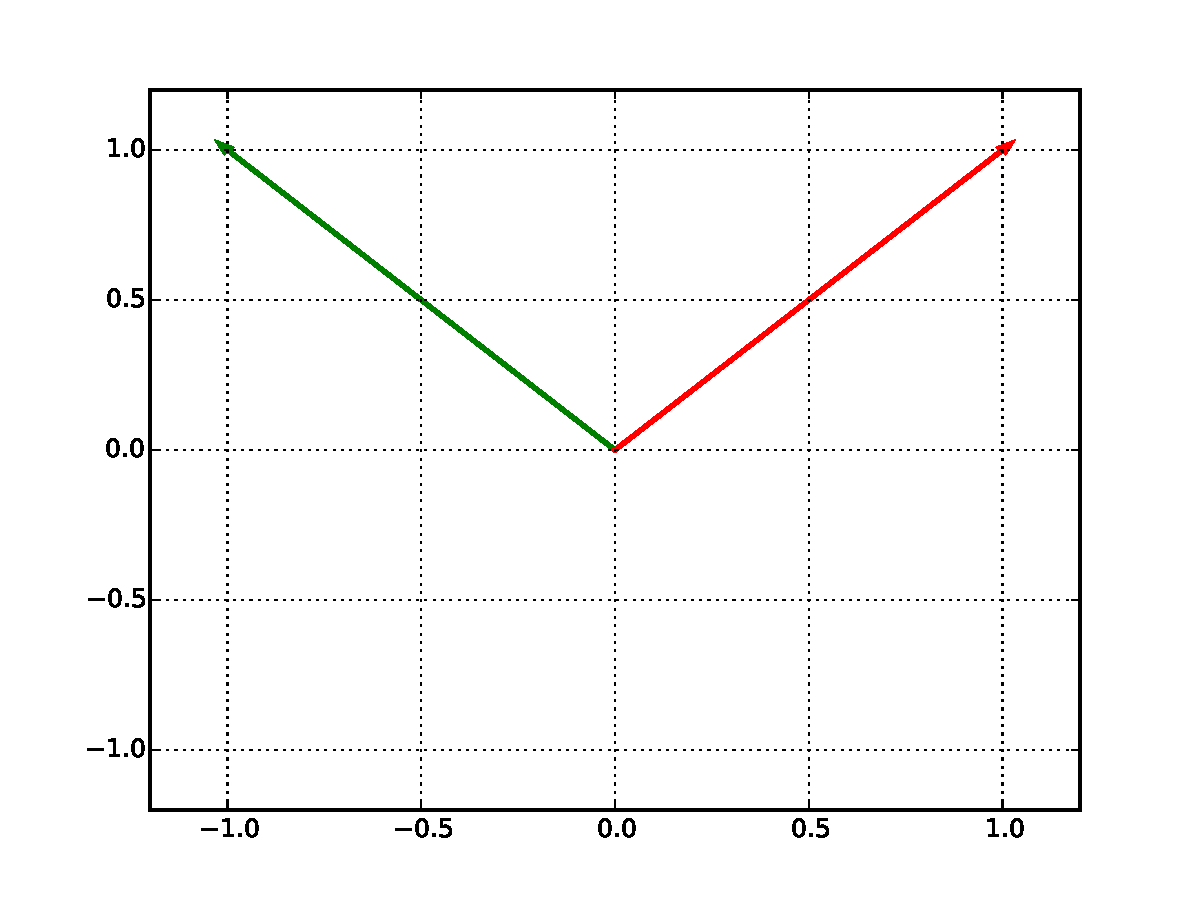
\includegraphics[width=\linewidth]{figs/ex7_1_3.pdf}

\begin{verbatim}
A= Matrix(2, 2, [3, 1, 1, 3])
evecs= A.eigenvects()

plt.subplot()
plt.xlim(-1.2, 1.2)
plt.ylim(-1.2, 1.2)
plt.arrow(0, 0, float(evecs[0][2][0][0]), float(evecs[0][2][0][1]),
    linewidth= 2, color= 'g')
plt.arrow(0, 0, float(evecs[1][2][0][0]), float(evecs[1][2][0][1]),
    linewidth= 2, color= 'r')
plt.grid()
plt.savefig('figs/ex7_1_3.pdf')
plt.close()
\end{verbatim}

\subsubsection{Exercise 7.1.4}
% ----------------------------

What is the effect of multiplying matrix $\mathbf{A}= \left[\begin{matrix}5 & -2\\7 & -4\end{matrix}\right]$ by its eigenvector. Plot the eigenspace
and compute a basis vector for each eigenspace.

Eigenvalues, multiplicity and eigenvectors:

$$
\left [ \left ( -2, \quad 1, \quad \left [ \left[\begin{matrix}\frac{2}{7}\\1\end{matrix}\right]\right ]\right ),
\quad \left ( 3, \quad 1, \quad \left [ \left[\begin{matrix}1\\1\end{matrix}\right]\right ]\right )\right ]
$$

Multiplying (transforming) the eigenvector by the matrix has the same effect as
extending the eigenvector by a factor $\lambda$, there is no change in direction
of the eigenvector. \textit{I.e.} $\mathbf{Au} = \mathbf{\lambda u}$.

The basis for the eigenspace are the eigenvectors
$\mathbf{u} = \left[\begin{matrix}\frac{2}{7}\\1\end{matrix}\right], \quad
\mathbf{v}= \left[\begin{matrix}1\\1\end{matrix}\right]$. Which means \textbf{u}
is the basis vector for $\lambda= -2$ and \textbf{v} is the basis vector for $\lambda= 3$.
They are a basis because every vector in their space can be created by linear combination
of these vector. In fact, every segment sitting on the line $[2/7 \quad 1]^T$ can be
obtained by multiplying $[2/7 \quad 1]^T$ by an appropriate scalar (and the same for any segment sitting
on \textbf{u}).

\begin{verbatim}
A= Matrix(2,2, [5, -2, 7, -4])
evecs= A.eigenvects()
ev= [x[2][0] for x in evecs]

# Au = lambda*u
u= evecs[0][2][0]
lamu= evecs[0][0]
A* u == lamu * u ## True

v= evecs[1][2][0]
lamv= evecs[1][0]
A* v == lamv * v ## True
\end{verbatim}

\subsection{Properties of eigenvalues and eigenvectors}
% =====================================================

\subsubsection{Exercise 7.2.3}
% ----------------------------

The characteristic equation is the characteristic polynomial equated to zero.

The characteristic polynomial ($p(\lambda)$) for a 2x2 matrix \textbf{A} is
$p(\lambda) = det(\mathbf{A} - \lambda \mathbf{I})$ and it is equivalent
to $p(\lambda) = \lambda^2 - tr(\mathbf{A}) \lambda + det(\mathbf{A})$, as shown below.

\begin{verbatim}
a,b,c,d= symbols('a:d', real= True)
lamda= symbols('lambda', real= True)
A= Matrix(2, 2, [a, b, c, d])

charp= lamda**2 - A.trace() * lamda + A.det()
chareq= det(A - lamda * eye(2))
Eq(chareq.expand() - charp.expand()) # True
\end{verbatim}

Note that equality between polynomials is tested after \texttt{expand}ing them to canonical
form. Simply testing \texttt{charp - chareq} will not return 0 as it should. See also
\sympy \href{https://github.com/sympy/sympy/wiki/Faq}{FAQ}

\subsubsection{Exercise 7.2.4}
% ----------------------------

Given \textbf{A} a 2x2 matrix with $tr(\mathbf{A}) = 2a$ and $det(\mathbf{A}) = a^2$,
obtain the eigenvalue $\lambda$. 

Start from the characteristic polynomial $p(\lambda) = \lambda^2 - tr(\mathbf{A})\lambda + det(\mathbf{A})$
and substitute the values $tr(\mathbf{A}) = 2a$ and $det(\mathbf{A}) = a^2$. The resulting
equation $p(\lambda) = a d - b c + \lambda^{2} - \lambda \left(a + d\right)$ is solved
for $\lambda= a$. Therefore given the conditions above an eigenvalue of \textbf{A} is
$a$. Since $a$ is the only solution and the matrix is 2x2, than $a$ has multiplicity 2,
\textit{i.e.} it occurs twice.

\begin{verbatim}
a,b,c,d= symbols('a:d', real= True)
lamda= symbols('lambda', real= True)
A= Matrix(2, 2, [a, b, c, d])

charp= lamda**2 - A.trace() * lamda + A.det()
charp2= charp.subs(A.trace(), 2*a).subs(A.det(), a**2)
ev= solve(charp2, lamda) # [a]
\end{verbatim}

\subsubsection{Exercise 7.2.5}
% ----------------------------

For $\mathbf{A} = \left[\begin{matrix}1 & 0 & 0\\-3 & 1 & 0\\7 & 9 & 1\end{matrix}\right]$
obtain eigenvalues and eigenvectors. Write down a set of basis vectors.

Since this is a triangular matrix, the eigenvalues can be read from the main diagonal.
In this case $\lambda= 1$ with multiplicity 3. Consequently there is only one eigenvector
$\mathbf{v}= [0\ 0\ 1]^T$.

The basis is $\mathbf{x\ y\ z}= [0\ 0\ 1]^T$ which means that the eigenspace for
$\lambda= 1$ is the vertical axis $z$ in 3D space.

\begin{verbatim}
A= Matrix([[1, 0, 0], [-3, 1, 0], [7, 9, 1]])
ev= A.eigenvects()
\end{verbatim}

Note that in triangular matrices only the leading diagonal determines the eigenvalues/vectors.
The generic triangular matrix $\left[\begin{matrix}1 & 0 & 0\\a & 1 & 0\\b & c & 1\end{matrix}\right]$
has the same values as the matrix \textbf{A} above:

\begin{verbatim}
A1= Matrix([[1, 0, 0], [a, 1, 0], [b, c, 1]])
ev1= A.eigenvects() ## Same as above
ev == ev1 # True
\end{verbatim}

Note that if n eigenvalues are distinct then the corresponding eigenvectors are
linearly independent.

\subsection{Diagonalization}
% ==========================

Diagonalization is the process of converting an n x n matrix in a diagonal one. The
values on the diagonal matrix are the eigenvalues of the original matrix. Diagonal
matrices are much easier to work with then full matrices.

The power of matrices, useful in Markov models, is much simplified by means of
diagonalization since $\mathbf{D}^n$ is easy to compute if \textbf{D} is a diagonal
matrix.

Diagonalize \textbf{A} means that:

$$
\mathbf{P^{-1} A P = D} \quad and \quad
\mathbf{A = P D P^{-1}}
$$



That is, there exists a matrix \textbf{P} so that the multiplication above transforms
\textbf{A} into a diagonal matrix \textbf{D}. \textbf{P} is a matrix of eigenvectors
of \textbf{A}:

$$
\mathbf{A^m = P  D^m  P^{-1}}
$$

(that's why diagonalization appears in the chapter about eigenvalues/vectors).

\subsubsection{Exercise 7.3.1}
% ----------------------------

\begin{verbatim}
A= Matrix(2, 2, [1, 0, 0, 2])
evecs= [x[2][0] for x in A.eigenvects()]
P= Matrix(np.column_stack(evecs))
D= P.inv() * A * P
Eq(A, P * D * P.inv())

A= Matrix(2, 2, [2, 2, 1, 3])
evecs= [x[2][0] for x in A.eigenvects()]
P= Matrix(np.column_stack(evecs))
D= P.inv() * A * P
Eq(A, P * D * P.inv())
\end{verbatim}

\subsubsection{Exercise 7.3.2}
% ----------------------------

Find $\mathbf{A}^5$ for $\mathbf{A} = \left[\begin{matrix}2 & 2\\1 & 3\end{matrix}\right]$.

\begin{enumerate}
\item Find the eigenvectors of \textbf{A}. Put them in matrix \textbf{P} by column binding.
\item Get the eigenvalues of \textbf{A}. Put them along the diagonal matrix \textbf{D}.
\item Calculate power of \textbf{A} as $\mathbf{A}^m = \mathbf{PD^mP^{-1}}$ for $m= 5$. 
\end{enumerate}

We use \sympy \texttt{Matrix.eigenvects} to obtain eigenvectors/values.  For \textbf{A}
we have the list of tuples $\left [ \left ( 1, \quad 1, \quad \left [ \left[\begin{matrix}-2\\1\end{matrix}\right]\right ]\right ), \quad \left ( 4, \quad 1, \quad \left [ \left[\begin{matrix}1\\1\end{matrix}\right]\right ]\right )\right ]$.
Each tuple is (eigenvalue, multiplicity, eigenvector).

The matrix of eigenvectors is $\mathbf{P} = \left[\begin{matrix}-2 & 1\\1 & 1\end{matrix}\right]$
and the diagonal matrix of eigenvalues is $\mathbf{D} = \left[\begin{matrix}1 & 0\\0 & 4\end{matrix}\right]$

Now $\mathbf{A}^5$ is easy to compute as $\mathbf{A}^5 = \mathbf{P D^5 P^{-1}} =
\left[\begin{matrix}-2 & 1\\1 & 1\end{matrix}\right]
\left[\begin{matrix}1^5 & 0\\0 & 4^5\end{matrix}\right]
\left[\begin{matrix}- \frac{1}{3} & \frac{1}{3}\\\frac{1}{3} & \frac{2}{3}\end{matrix}\right] =
\left[\begin{matrix}342 & 682\\341 & 683\end{matrix}\right]$

\begin{verbatim}
A= Matrix(2, 2, [2, 2, 1, 3])

def powerMat(A, m):
    """Return the square matrix A to the power of m"""
    # Eigenvectors/values
    ev= A.eigenvects()
    P= Matrix(np.array([x[2][0] for x in ev])).transpose()
    D= diag(*[x[0] for x in ev])
    Am= P * D**Rational(m) * P.inv()
    return Am

A5= powerMat(A, 5)
    
## Check against SymPy
A**5 == A5 ## True
\end{verbatim}

For $\mathbf{A} = \left[\begin{matrix}3 & 0\\4 & 4\end{matrix}\right] ^ {-1/2} =
\left[\begin{matrix}\frac{\sqrt{3}}{3} & 0\\- \frac{4 \sqrt{3}}{3} + 2 & \frac{1}{2}\end{matrix}\right]$

Note the use of \texttt{Rational(-1/2)} required by \sympy to deal with rational
numbers.

\begin{verbatim}
A= Matrix(2, 2, [3, 0, 4, 4])
Am= powerMat(A, -1/2)
A**Rational(-1/2) == Am ## True
\end{verbatim}

\subsubsection{Exercise 7.3.4}
% ----------------------------

Determine whether the following matrices are diagonalizable.

To answer the question consider that:

\begin{itemize}
\item If an $n$ x $n$ matrix has $n$ distinct eigenvalues, than the corresponding
eigenvectors are \emph{linearly independent}.

\item If an $n$ x $n$ matrix has $n$ distinct eigenvalues then the matrix is diagonalizable.
\end{itemize}

Note that in some cases a matrix can be diagonalizable even if doesn't have $n$ distinct eigenvalues
(\emph{I.e.} the above is not an \emph{if and only if} condition).

For the identity matrix $\mathbf{A} = \left[\begin{matrix}1 & 0 & 0\\0 & 1 & 0\\0 & 0 & 1\end{matrix}\right]$
we have one eigenvalue $\lambda = 1$ with multiplicity 3 and eigenvectors
$\left [ \left[\begin{matrix}1\\0\\0\end{matrix}\right], \quad \left[\begin{matrix}0\\1\\0\end{matrix}\right], \quad \left[\begin{matrix}0\\0\\1\end{matrix}\right]\right ]$.

The matrix of eigenvectors therefore is $\mathbf{P} = \left[\begin{matrix}1 & 0 & 0\\0 & 1 & 0\\0 & 0 & 1\end{matrix}\right]$,
and the matrix of eigenvalues $\mathbf{P} = \left[\begin{matrix}1 & 0 & 0\\0 & 1 & 0\\0 & 0 & 1\end{matrix}\right]$.

The identity matrix is therefore diagonalizable even if the distinct eigenvalues is less
than the matrix dimension since $\mathbf{I} = \mathbf{A} = \mathbf{P D P^{-1}}$.

\begin{verbatim}
A= eye(3)
ev= A.eigenvects()
P= Matrix(np.column_stack(ev[0][2])).transpose()
D= diag(*[ev[0][0]]*A.rows)

A == P * D * P.inv() # True
\end{verbatim}

For $\mathbf{A} = \left[\begin{matrix}-1 & 2 & 3\\0 & 2 & 5\\0 & 0 & 8\end{matrix}\right]$
the matrix is triangular and therefore the eigenvalues are on the leading diagonal.
The eigenvalues are distinct and therefore the matrix is diagonalizable.

\begin{verbatim}
A= Matrix([[-1, 2, 3], [0, 2, 5], [0, 0, 8]])
ev= A.eigenvects()
P= Matrix(np.array([x[2][0] for x in ev])).transpose()
D= diag(*[x[0] for x in ev])
A == P * D * P.inv()
\end{verbatim}

\subsection{Diagonalization of Symmetric Matrices}
% ================================================

Some useful definitions and properties:

\begin{itemize}

\item A matrix is symmetric if $\mathbf{A = A^T}$.

\item Symmtric matrices can be diagonalized by an orthogonal matrix. 

\item Orthogonality: Two vectors are orthogonal, \emph{i.e.} their angle is 90$^{\circ}$,
if their inner (dot) product is zero:

$$
\mathbf{u \cdot v} = 0
$$

Note that orthogonality makes sense for vectors of any dimension even if geometrically
vectors of length $>3$ cannot be visualized

\item The distinct eigenvalues of a symmetric matrices have corresponding eigenvectors
which are othogonal. \emph{N.B.} the covariance matrix is symmetric.

For example, matrix $\mathbf{M}= \left[\begin{matrix}-5 & 4 & 2\\4 & -5 & 2\\2 & 2 & -8\end{matrix}\right]$
is symmetric and has the following eigenvalues, multiplicity and eigenvectors
$$\left [ \left ( -9, \quad 2, \quad \left [ \left[\begin{matrix}-1\\1\\0\end{matrix}\right],
\quad \left[\begin{matrix}- \frac{1}{2}\\0\\1\end{matrix}\right]\right ]\right ),
\quad \left ( 0, \quad 1, \quad \left [ \left[\begin{matrix}2\\2\\1\end{matrix}\right]\right ]\right )\right ]$$

Eigenvalue -9 has multiplicity 2 (two eigenvectors), and these are \emph{not} orthogonal.
However, these two eigenvectors are orthogonal to the eigenvector with eigenvalue
0: $\left[\begin{matrix}-1\\1\\0\end{matrix}\right] \cdot \left[\begin{matrix}- \frac{1}{2}\\0\\1\end{matrix}\right]  = 1/2$ and
$\left[\begin{matrix}2\\2\\1\end{matrix}\right] \cdot \left[\begin{matrix}-1\\1\\0\end{matrix}\right] =
\left[\begin{matrix}2\\2\\1\end{matrix}\right] \cdot \left[\begin{matrix}- \frac{1}{2}\\0\\1\end{matrix}\right] = 0$

\begin{verbatim}
M= Matrix([[-5, 4, 2],
           [4, -5, 2],
           [2, 2, -8]])
ev= M.eigenvects()
u= ev[0][2][0]
v= ev[0][2][1]
z= ev[1][2][0]

u.dot(v) == 0 # False
z.dot(u) == 0 # True
z.dot(v) == 0 # True
\end{verbatim}

\item A matrix \textbf{Q} is \textbf{orthogonal} if its column vectors are orthogonal to each other and
of norm 1, \emph{i.e.} they orthonormal.

\item \textbf{Orthogonal diagonalization} of matrix \textbf{A} means the following decomposition

$$
\mathbf{A = Q^{-1}DQ = Q^TDQ}
$$

As before, \textbf{Q} column-binds the normalized eigenvectors of \textbf{A}. \textbf{D}
is a diagonal matrix with the eigenvalues of \textbf{A} along the leading diagonal.

\item Because of the diagonalization $\mathbf{A = Q^{-1}DQ = Q^TDQ}$ symmetric
matrices are easy to diagonalize since we don't need to invert \textbf{Q}, an
expensive operation, we just need to transpose \textbf{Q}.
\end{itemize}

\subsubsection{Exercise 7.4.1}
% ----------------------------

Find and orthogonal matrix \textbf{Q} which diagonalizes the following matrices.

\begin{itemize}
\item Find eigenvectors of \textbf{A}, column-bind them
\end{itemize}

\begin{verbatim}

def normalize(v):
    """Normalize vector v
    """
    vsq= sqrt(sum([x**2 for x in v]))
    return 1 / vsq * v 

def getQD(M):
    """Return a tuple of
    * Matrix of normalized eigenvectors of M column binded
    * Diagonal matrix of eigenvalues of A
    """
    assert M == M.transpose() # Check M is symmetric.
    ev= M.eigenvects()
    eigval_lst= []
    eigvec_lst= []
    for vmv in ev:
        eigvec= vmv[2]
        for v in eigvec:
            # For each eigenvector in this eigenvalue.
            eigval_lst.append(vmv[0])
            vnorm= normalize(v)
            eigvec_lst.append(list(vnorm))
    Q= Matrix(eigvec_lst).transpose()
    assert Q * Q.transpose() == eye(A.rows) # Test Q is orthogonal
    D= diag(*eigval_lst)
    return (Q, D)

A= Matrix(2, 2, [1, 0, 0, 2])
Q,D= getQD(A)
Q.transpose() * A * Q == D # True

# ----

A= Matrix(2, 2, [5, 12, 12, -5])
Q,D= getQD(A)
Q.transpose() * A * Q == D # True

# ----

A= Matrix([[5, sqrt(12)], [sqrt(12), 1]])
Q,D= getQD(A)
Q.transpose() * A * Q == D # True
\end{verbatim}


\subsection{Singular Value Decomposition}
% =======================================

Useful concepts and properties:

\begin{itemize}
\item Eigenvalues/vectors can be obtained only for square matrices, so if \textbf{A}
is not square we can't get eigenvalues/vectors.
\item Good news is $\mathbf{A^TA}$ is square \emph{and} symmetric! This means that
$\mathbf{A^TA}$ can be easily diagonalized.
\item The eigenvalues of $\mathbf{A^TA}$ are either positive or zero.
\end{itemize}

\subsubsection{Exercise 7.5.1}
% ----------------------------

Decompose \textbf{A} so that

$$
\mathbf{A = UDV^T}
$$

\begin{itemize}

\item Singular values of \textbf{A}: The square root of the eigenvalues of $\mathbf{A^TA}$, denoted
$\sigma_1, \sigma_2, \dots, \sigma_n$ with $n$ the number of columns in \textbf{A}.
The eigenvectors corresponding to $\sigma_i$, $\mathbf{v_i}$ give the equation
$$
\mathbf{\sigma_i u_i = Av_i}
$$

$\sigma$s and vectors \textbf{v} should be in order largest to smallest.

\item $\mathbf{U}$ Matrix of vectors normalized $\mathbf{u_i}$ from above.

\item $\mathbf{D}$: Diagonal matrix of singular values of \textbf{A}.

$$
\mathbf{D} = \left[\begin{matrix}\sigma_{1} & 0 & 0\\0 & \sigma_{2} & 0\\0 & 0 & \sigma_{n}\end{matrix}\right]
$$

Take care of the size of \textbf{D}. If \textbf{A} is rectangular with more rows than columns, than the diagonal is filled up with zeros.


\item $\mathbf{V}$: Matrix of eigenvectors of $\mathbf{A^TA}$ of size $n$:

$$
\mathbf{V = (v_1\ v_2 \dots v_n)}
$$

\end{itemize}

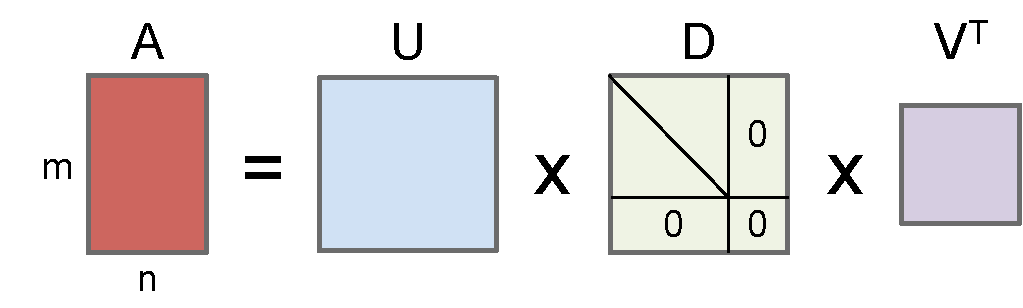
\includegraphics[width=0.7\linewidth]{figs/SVD_UDV.pdf}

For matrix \textbf{A}
$$
\mathbf{A} = \left[\begin{matrix}1 & 0\\0 & 1\\1 & 2\end{matrix}\right]
$$

We have:
$$
\mathbf{A^TA} = \left[\begin{matrix}2 & 2\\2 & 5\end{matrix}\right]
$$

$\sigma$s are $\left [ \sqrt{6}, \quad 1\right ]$ which go in \textbf{D} matrix

$$
\mathbf{D} = \left[\begin{matrix}\sqrt{6} & 0\\0 & 1\end{matrix}\right]
$$

Matrix \textbf{U} has the \textbf{u} vectors:

$$
\mathbf{U} = \left[\begin{matrix}\frac{\sqrt{30}}{30} & - \frac{2 \sqrt{5}}{5}\\\frac{\sqrt{30}}{15} & \frac{\sqrt{5}}{5}\\\frac{\sqrt{30}}{6} & 0\end{matrix}\right]
$$

Finally, \textbf{V}:

$$
\mathbf{V} = \left[\begin{matrix}\frac{\sqrt{5}}{5} & - \frac{2 \sqrt{5}}{5}\\\frac{2 \sqrt{5}}{5} & \frac{\sqrt{5}}{5}\end{matrix}\right]
$$

Check $\mathbf{A = UDV^T}$.

\emph{This code is not always correct!}

\begin{verbatim}
A= Matrix([[1, 0], [0, 1], [1, 2]])

# Singular values and Matrix D
AtA= A.T * A
svv= sorted(AtA.eigenvects(), key= lambda x: x[0], reverse= True)
sigmas= [sqrt(x[0]) for x in svv]
atavecs= [x[2][0] for x in svv]
atavecs= [normalize(x) for x in atavecs]
          
U= []
D= []
V= []
for v, s in zip(atavecs, sigmas):
    if s == 0:
        continue
    u_i= A*v / s    # u_1 = A * v_i
    U.append(u_i)
    D.append(s)
    V.append(v)
U= Matrix(np.array(U)).T
D= diag(*D)
V= Matrix(np.array(V)).T

# Check decomposition
A == U * D * V.T
\end{verbatim}

\subsubsection{Interpreting the decompostion}
% -------------------------------------------

Since a matrix \textbf{A} can be thought of a transformation, we can ask the question
of what operations lead to such a transformation.

The SVD decomposes \textbf{A} into three simple transformations
\footnote{From \href{http://en.wikipedia.org/wiki/Singular_value_decomposition}{Wikipedia Singular value decomposition}}:

\begin{itemize}
    \item An initial rotation $\mathbf{V^T}$. \textbf{V} is a symmetric matrix, so its action is to rotate.
    \item A scaling \textbf{D} along the coordinate axes. \textbf{D} is diagonal, so its action is to stretch or shrink, without rotating or shearing.
    \item A final rotation \textbf{U}. The lengths $\sigma_1$ and $\sigma_2$ of the semi-axes are the singular values of M.
\end{itemize}

See also the applet at \href{http://mathforum.org/mathimages/index.php/Transformation_Matrix}{Transformation Matrix} for some effects of matrix transformation 
\section{Appendix}
% ****************

\subsection{Plotting with \texttt{matplotlib.pyplot}}
% ===================================================

The documentation of \texttt{matplotlib} and its modules is quite extensive
but it doesn't give a simple overview of how graphics are organized. Therefore this
section outlines the idea behind \texttt{pyplot} graphics and its components. 

\cmd{pyplot} is a layer on \texttt{matplotlib} to provide graphic facilities
similar to Matlab. \texttt{pyplot} appears to be the preferred way to plot
graphics in \texttt{python/matplotlib}. See also \href{http://matplotlib.org/faq/usage_faq.html}{matplotlib usage} and 
the tutorial \href{https://github.com/ericliang/matplotlib/blob/master/trunk/scipy06/oo_resources/leftwich_tut.txt}
{Getting Started With Matplotlib}.

So, first import the \cmd{pyplot} module:

\begin{verbatim}
import matplotlib.pyplot as plt
\end{verbatim}

and get some dummy data to play with:

\begin{verbatim}
import numpy as np

x= np.array([1, 2, 3, 4])
y= x**2
\end{verbatim}

Here \texttt{x} and \texttt{y} are numpy arrays, although \texttt{pyplot} accepts
any iterable.

\subsubsection{Figure}
% --------------------------
\begin{verbatim}
fig= plt.figure()
\end{verbatim}

\cmd{matplotlib.figure.Figure()} is the top level of a graphics where everything starts
and it is therefore the equivalent of a blank sheet of paper where you draw the plot on. Use \texttt{figure}
to set among other things the \textbf{size} of the figure (in inches) and the \textbf{dpi} resolution,
if applicable. More or less the call \texttt{fig= plt.figure()} is equivalent to
\texttt{R}'s \texttt{g<- ggplot()}. \texttt{figure()} can be called with only default parameters;
in fact, a call to \texttt{Figure} can be skipped altogheter (see below). 

\subsubsection{Axis}
% ------------------

\begin{verbatim}
axes= fig.add_subplot(1, 3, 2)
\end{verbatim}

To draw on a \texttt{Figure} object you need to put a set of \cmd{Axes} where you actually
draw stuff.

\texttt{Axes} can be put with \cmd{.add\_subplot} or \cmd{.add\_axes}. \texttt{add\_subplot}
is similar to \texttt{R} \texttt{par(mfrow= c(n, m))} in that it divides the figure
in \emph{n} rows and \emph{m} columns. The third argument in \texttt{add\_subplot} states
which subplot should be drawn upon. \emph{E.g.} \texttt{fig.add\_subplot(1, 3, 2)}
sets one row, three columns, and draws in the middle subplot (number 2).

Alternatively \cmd{.add\_axes} can be used to specify the characteristics of the
plotting box. It's roughly equivalent to \texttt{R} \texttt{par(mar= c(a, b, c, d))}
in that you set the position of the axes relative to the overall figure. It can also
be used to add plot on top of each other, like figure insets.

The \cmd{Axes} object can be used to control graphic parameters like x- and y-limits,
the axis labels and the plot title. It controls more or less what you can control with \texttt{R}'s \texttt{par()}.

As for \texttt{Figure}, you can add a subplot with only default arguments or skip
the call altogether.

\subsubsection{Plotting}
% ----------------------

\begin{verbatim}
axes.plot(x, y)
\end{verbatim}

Drawing is realized by adding stuff to the \texttt{Axes} object, typically by means
of \cmd{plot()} function. Similar to \texttt{R plot()}, with \texttt{plot} you can
set the plotting style (line, point), colour, etc. See \href{http://matplotlib.org/api/pyplot_api.html#matplotlib.pyplot.plot}
{pyplot.plot} for documentation of setting line styles and plotting features.

\subsubsection{Rendering}
% ----------------------

\begin{verbatim}
fig.savefig('filename.pdf')
fig.show()
plt.close()
\end{verbatim}

The actual plot is visualized with the \cmd{show()} method and saved to file with
\cmd{savefig()} method. By default, file format is deduced from file extension.
Finally, call \cmd{close} to close the grahic device(s).

\subsubsection{In practice...}
% ----------------------------

In practice you can take shortcuts to create plots. It is not strictly necessary
to explicitly set up a \texttt{Figure} and \texttt{Axes} object.

\begin{verbatim}
plt.plot(x, y, 'r--', lw= 2)
plt.plot(x, y, 'bo', markersize=12)
plt.xlabel('x-lab')
plt.xlim([0, 5])
plt.rc('font', size= 20)
plt.grid()
plt.savefig('figs/app_simple.pdf', bbox_inches= 'tight')
plt.show()
\end{verbatim}

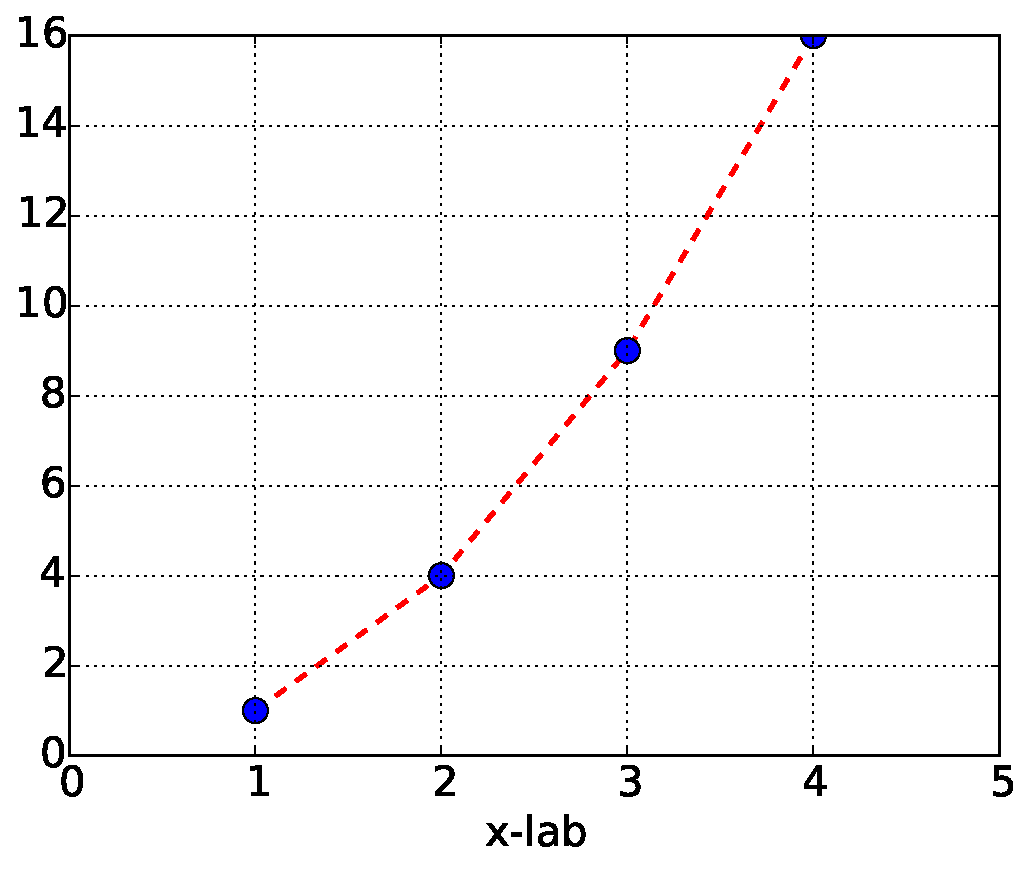
\includegraphics[width=0.5\linewidth]{figs/app_simple.pdf}

For simple plots, you can just call \cmd{plt.plot()} with the data to plot and
optional graphic paramaters. The bare minimum to see an xy-plot is just
\texttt{plt.plot(x, y); plt.show()}

Note that you keep adding features using \texttt{plt.<feature>},
then when you call \texttt{savefig} or \texttt{show} everything comes together.
In contrast to \texttt{R}, the order with which you add these features doesn't
matter. However, if you want to save to file \emph{and} show on screen, remember
to call \texttt{savefig} first and \texttt{show} then.

\begin{verbatim}
plt.rc('font', size= 8)
fig, axlst = plt.subplots(1, 3, sharex=True, sharey= True)
axlst[0].plot(x, y)
axlst[1].plot(x, y*2)
axlst[2].plot(x, y*3)
fig.subplots_adjust(wspace= 0.1)
fig.set_size_inches(18/2.54, 6/2.54)
fig.savefig('figs/app_subplot.pdf')
fig.show()
\end{verbatim}

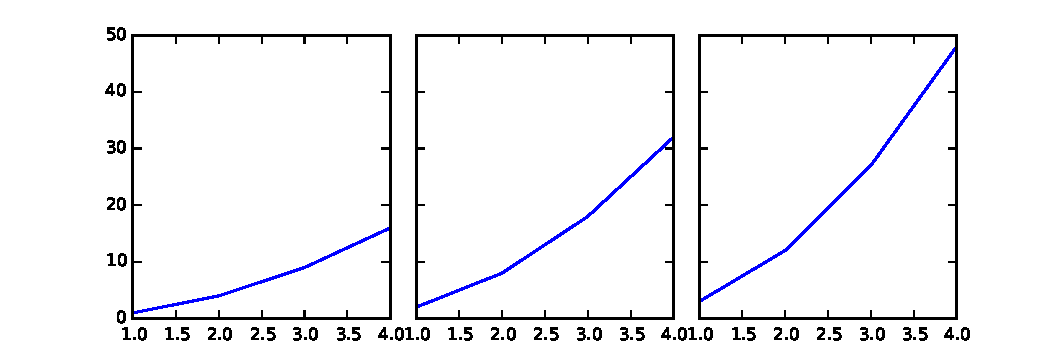
\includegraphics[width=\linewidth]{figs/app_subplot.pdf}

For multiple plots it might be best to set up the \texttt{Figure} object and the
list (array actually) of subplots in one call to \cmd{plt.subplots()}. Each element
of the array contains an \texttt{Axes} object that can be individually populated.
The \texttt{Axes}'s can be juxtaposed by playing with the method \cmd{Figure.subplots\_adjust}.
For example to set the spacing. 

\subsubsection{Example}
% ---------------------

\begin{verbatim}

fig= plt.figure()
ax1= fig.add_subplot(1, 3, 1)
ax1.plot(x, y, 'r--')
ax2= fig.add_subplot(1, 3, 2)
ax2.plot(x, y, 'pg')
ax3= fig.add_subplot(1, 3, 3)
ax3.plot(x, y, 'p')
for i, txt in enumerate(x):
    ax3.annotate(txt, (x[i], y[i]))
fig.show()
\end{verbatim}

\subsection{Principal components}
% ===============================

\dots

For interpretation of eigenvalues and eigenvectors of a covariance matrix see
http://www.visiondummy.com/2014/04/geometric-interpretation-covariance-matrix/

\subsection{PageRank}
% ===================

Google ranks pages predominantly according to two criteria: 1) Number of links a page
receives, \emph{i.e.} many other pages rerfers to it, or in other words it is 'cited' very often;
2) Incoming links are not all equal, incoming links from important pages are more
important, \emph{i.e.} being 'cited' by a very important page counts more.

See also \href{http://www.math.cornell.edu/~mec/Winter2009/RalucaRemus/Lecture3/lecture3.html}{The Mathematics of Google Search}

Stochastic matrix, \textit{i.e.} where column sums equal 1, describing how node weights
are distibuted.

\begin{equation}
\mathbf{A} = \left[\begin{matrix}0 & 0 & 1.0 & 0.5\\0.3 & 0 & 0 & 0\\0.3 & 0.5 & 0 & 0.5\\0.3 & 0.5 & 0 & 0\end{matrix}\right]
\end{equation}

\begin{itemize}
\item Each \textbf{column} describes how each node distributes its weight.

For example, $1^{st}$ column, $[0\ \frac{1}{3}\ \frac{1}{3}\ \frac{1}{3}]^T$, says that node $x_1$ gives 0 of its
weight to itself (of course), 1/3 to $x_2$, 1/3 to $x_3$, and 1/3 to $x_4$;
$4^{th}$ column describes node $x_4$ and it says that 1/2 weight is given to $x_1$,
0 to $x_2$, 1/2 to $x_3$, and 0 to itself.

\item Each \textbf{row} describes the weight or score of each node, since it is the SUM
of all the node weights.

For example, $1st$ row is the score for node $x_1$. $x_1$
receives 0 from itself (of course), 0 of the weight of $x_2$, 1 (\textit{i.e. all})
of the weight from $x_3$, and 1/2 of the weight from $x_4$.
\end{itemize}

So matrix \textbf{A} tells the \textit{proportion} of weight to and from nodes. The question
is: \emph{How much each node weighs?} If all the nodes had the same weight the row sums
of \textbf{A} would give the page rank already. However, we want to give more weight
to pages that have many incoming links and/or incoming links from high ranking pages.
For example, node $x_1$ receives all of the weight from $x_3$ (1) and half of the weight
from $x_4$ (0.5). But how much do $x_3$ and $x_4$ weigh?

The assign weights to nodes we need to solve the linear system where the LHS is
matrix \textbf{A} and RHS is the vector of weights (ranks) we want to find out:

\begin{equation}
\left[\begin{matrix}
0 x_1 + 0 x_2 + 1 x_{3} + 0.5 x_{4} \\
0.3 x_{1}  + 0 x_2 + 0 x_3 + 0 x_4 \\
0.3 x_{1} + 0.5 x_{2} + 0 x_3 + 0.5 x_{4} \\
0.3 x_{1} + 0.5 x_{2} + 0 x_3 + 0 x_4
\end{matrix}\right] =
\left[\begin{matrix}x_{1}\\ x_{2}\\x_{3}\\x_{4}\end{matrix}\right]
\end{equation}

This is equivalent to finding the eigenvector of \textbf{A} for the eigenvalue 1.
In fact see that if we set $\left[\begin{matrix}x_{1}\\x_{2}\\x_{3}\\x_{4}\end{matrix}\right] = \mathbf{u}$,
we have in matrix notation:

\begin{equation}
\mathbf{Au = \lambda u}; \quad and\ for\ \lambda = 1: \quad \mathbf{Au = u}; 
\end{equation}

which is the definition of eigenvectors/values. Note that since \textbf{A} is
stochastic the largest eigenvalue is always 1 \footnote{see also
\href{http://math.stackexchange.com/questions/40320/proof-that-the-largest-eigenvalue-of-a-stochastic-matrix-is-1}
{proof that the largest eigenvalue of a stochastic matrix} on Math Stack Exchange.}.

In this example the eigenvector for $\lambda = 1$ is $\mathbf{u} = \left[\begin{matrix}1\\0.33\\0.75\\0.5\end{matrix}\right]$.
We can normalize the scores to sum to 1 and obtain the pageRank
$PR =
\left[\begin{matrix}x_{1}\\x_{2}\\x_{3}\\x_{4}\end{matrix}\right] =
\left[\begin{matrix}0.39\\0.13\\0.29\\0.19\end{matrix}\right]$

Represent the web as a grpah and implement it as a dictionary of dictionaries. The outer dictionary has pages
(nodes) as keys. The value of each key (page) is a dictionary of outgoing links.
This inner dictionary has key: The arraival page, value: The weight transferred to
that page.

\begin{verbatim}
graph= {
    1: {2: 0, 3: 0, 4: 0},
    2: {3: 0, 4: 0},
    3: {1: 0},
    4: {1: 0, 3: 0}
}

# Assign weights to pages. Outgoing links:
for p in graph:
    pout= graph[p]
    for w in pout:
        pout[w]= 1.0 / len(pout)

# Matrix representation
pages= sorted(graph.keys())
A= np.array(zeros(len(pages), len(pages)))
for ci in range(len(pages)):
    page= graph[pages[ci]]
    for ri in range(len(pages)):
        outk= pages[ri]
        if outk in page:
            A[ri][ci]= page[outk]
A= Matrix(A)

# Solve A * u = u in order to get the ranks u:
u= Matrix(symbols('x1:%s' %(A.cols+1)))
Au= Eq(A*u, u)
sols= solve(Au.subs(x1, 1), u[1:])
sols[x1]= 1

# Or get all eigenvects, but slower since it calculates all of them:
A.eigenvects()[0]

# Normalize ranks to sum to 1
s= sum(sols.values())
pageRank= {}
for x in sols:
    pageRank[x]= sols[x]/s

PR= Matrix([pageRank[x] for x in u])

# Test we did it right
Eq(A * PR, PR) # True

\end{verbatim}

What if a page has no outgoing links? For example
\footnote{From J. Hefferon - Linear Algebra, Topic: Page Ranking}, in this graph
page 4 has no outgoing links:

\begin{verbatim}
graph= {
    1: {2:0},
    2: {3: 0},
    3: {1: 0, 2: 0, 4: 0},
    4: {}
}
\end{verbatim}

In this case we can imaging that a surfer reaching page 4 will move at random to
any other page. \emph{I.e.} we distribute the weight of page 4 uniformaly across
all the other pages:

\begin{verbatim}
for p in graph:
    pout= graph[p]
    if pout == {}:
        # If a page has no outgoing links distribute its weight across all web 
        for x in graph:
            graph[p][x]= 1.0 / len(graph)
    else:
        for w in pout:
            pout[w]= 1.0 / len(pout)
        graph[p]= pout
\end{verbatim}

This web looks like:

\begin{verbatim}
graph= 
{1: {2: 1.0},
 2: {3: 1.0},
 3: {1: 0.33, 2: 0.33, 4: 0.33},
 4: {1: 0.25, 2: 0.25, 3: 0.25, 4: 0.25}}
\end{verbatim}

As above, transform the graph in a stochastic matrix:

$$
\mathbf{A} = \left[\begin{matrix}0 & 0 & 0.33 & 0.25\\1.0 & 0 & 0.33 & 0.25\\0 & 1.0 & 0 & 0.25\\0 & 0 & 0.33 & 0.25\end{matrix}\right]
$$

\begin{verbatim}
pages= sorted(graph.keys())
A= np.array(zeros(len(pages), len(pages)))
for ci in range(len(pages)):
    page= graph[pages[ci]]
    for ri in range(len(pages)):
        outk= pages[ri]
        if outk in page:
            A[ri][ci]= page[outk]
A= Matrix(A)
\end{verbatim}

Obtain eigenvector for $\lambda= 1$ and normalize to have ranks to sum to 1
$$
PR = \left[\begin{matrix}0.16\\0.32\\0.36\\0.16\end{matrix}\right]
$$

Remember that there is an infinite number of eigenvectors belonging to an eigenvalue.
In fact we talk about \emph{eigenspace}. For convenience we choose the eigenvector
whose sum is 1.

\begin{verbatim}
def rankMatrix(A):
    """Return page ranks for matrix of weights A"""
    u= Matrix(symbols('x1:%s' %(A.cols+1)))
    Au= Eq(A*u, u)
    Au= Au.subs(x1, 1) # This sub is arbitrary, any real will do.
    sols= solve(Au, u[1:])
    sols[x1]= 1
    
    s= sum(sols.values())
    pageRank= {}
    for x in sols:
        pageRank[x]= sols[x]/s
    PR= Matrix([pageRank[x] for x in u])
    return PR
\end{verbatim}

Google edits the page rank matrix \textbf{A} to add some randomess in the behaviour
of the surfer. That is, a surfer every now and then might jump to a page not linked
in to the current one. The probability of jumping to an unlinked page is $\alpha$,
typically between 0.85 and 0.99.
To model this behaviour we edit the weight matrix \textbf{A} as follow:

\begin{itemize}
\item Edit the weights in weight matrix \textbf{A} by multiplying by the correction
factor $\alpha$, $\mathbf{A_{rnd}} = \alpha \mathbf{A}$.

\item Add to the corrected matrix $\alpha\mathbf{A}$ weights so that it returns to
be stochastic, \emph{i.e.} add $(1 - \alpha) \mathbf{R}$ where \textbf{R} is a matrix
of the same dim as \textbf{A} and with column sums 1.
\end{itemize}

Putting it all together, we obtain the \emph{Google matrix} \textbf{G} with the \emph{linear
combination}:

$$
\mathbf{G} = \alpha \mathbf{A} + (1 - \alpha) \mathbf{R}
$$

For this example:

$$
\mathbf{G} =
\alpha \left[\begin{matrix}0 & 0 & 0.33 & 0.25\\1.0 & 0 & 0.33 & 0.25\\0 & 1.0 & 0 & 0.25\\0 & 0 & 0.33 & 0.25\end{matrix}\right] +
(1 - \alpha) \left[\begin{matrix}0.25 & 0.25 & 0.25 & 0.25\\0.25 & 0.25 & 0.25 & 0.25\\0.25 & 0.25 & 0.25 & 0.25\\0.25 & 0.25 & 0.25 & 0.25\end{matrix}\right] =
$$

$$
\left[\begin{matrix}0 & 0 & 0.28 & 0.2125\\0.85 & 0 & 0.28 & 0.2125\\0 & 0.85 & 0 & 0.2125\\0 & 0 & 0.28 & 0.2125\end{matrix}\right] +
\left[\begin{matrix}0.0375 & 0.0375 & 0.0375 & 0.0375\\0.0375 & 0.0375 & 0.0375 & 0.0375\\0.0375 & 0.0375 & 0.0375 & 0.0375\\0.0375 & 0.0375 & 0.0375 & 0.0375\end{matrix}\right] =
\left[\begin{matrix}0.0375 & 0.0375 & 0.32 & 0.25\\0.8875 & 0.0375 & 0.32 & 0.25\\0.0375 & 0.8875 & 0.0375 & 0.25\\0.0375 & 0.0375 & 0.32 & 0.25\end{matrix}\right]
$$

The page ranks now become $PR_{\alpha=0.85} = \left[\begin{matrix}0.17 \\0.36 \\0.34 \\0.17 \end{matrix}\right]$.

Note that if $\alpha = 1$ than there is no randomess at all. If $\alpha = 0$ instead
the surfing is complete random and the page ranks become $PR_{\alpha=1} = \left[\begin{matrix}0.25\\0.25\\0.25\\0.25\end{matrix}\right]$

\begin{verbatim}
def googleRank(A, alpha= 0.85):
    """Ranks pages in weight matrix A after having add some random surfing
    behaviour alpha"""
    R= Matrix(A.rows, A.cols, [1/A.cols] * A.rows * A.cols)
    G = alpha * A + (1 - alpha) * R
    PR= rankMatrix(G)
    return PR

googleRank(A, 0.85)
\end{verbatim}

\subsection{Line of best fit (least squares)}
% ===========================================

\dots


\end{document}
